\documentclass[12pt]{extarticle}
\usepackage[paperwidth=15in,paperheight=7.2in]{geometry}
\usepackage{amsmath}
\usepackage{hyperref}
\usepackage{multirow}
\usepackage{pdfpages}
\usepackage[utf8]{inputenc}
\title{Kaon mixing: chiral and continuum extrapolations}
\author{R Mukherjee}
\date{\today}
\begin{document}
\maketitle
\tableofcontents
\clearpage
\begin{figure}
\centering
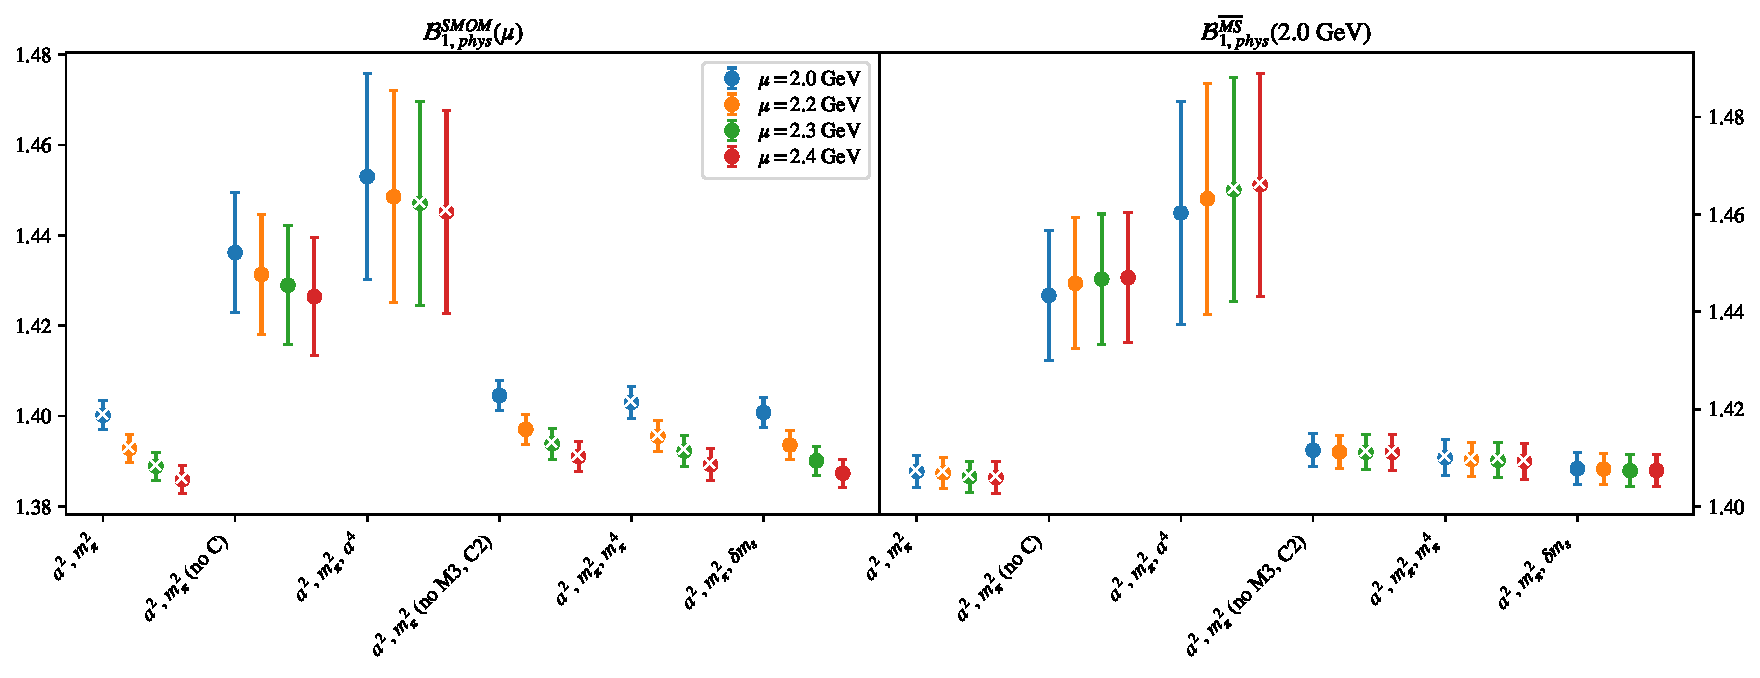
\includegraphics[page=1, width=1.1\textwidth]{VVpAA/NPR/fit_summary_bag.pdf}
\caption{$\mathcal{B}_{1}$\\(left) $\mathcal{B}_{phys}$ in RI/SMOM scheme from fit variations (fits with $p$-value $<0.05$ marked with ``$\times$"). \\(right) $\mathcal{B}_{phys}$ in $\overline{MS}$ computed using $\mathcal{B}^{\overline{MS}} = R^{\overline{MS}\leftarrow SMOM}(2.0)\sigma_{npt}(2.0,\mu) \mathcal{B}^{SMOM}(\mu)$.}
\end{figure}
\clearpage
\begin{figure}
\centering
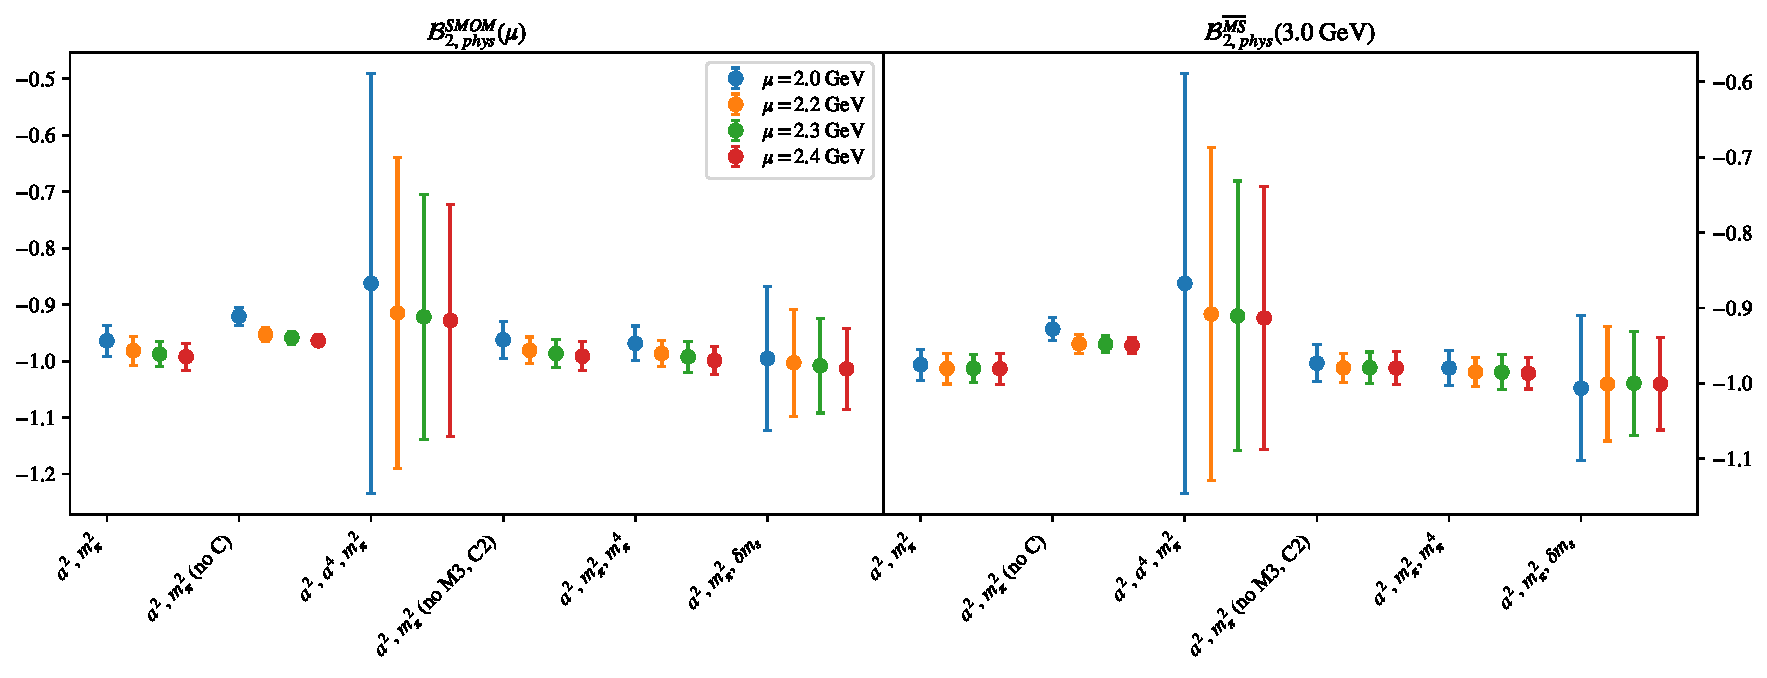
\includegraphics[page=1, width=1.1\textwidth]{VVmAA/NPR/fit_summary_bag.pdf}
\caption{$\mathcal{B}_{2}$\\(left) $\mathcal{B}_{phys}$ in RI/SMOM scheme from fit variations (fits with $p$-value $<0.05$ marked with ``$\times$"). \\(right) $\mathcal{B}_{phys}$ in $\overline{MS}$ computed using $\mathcal{B}^{\overline{MS}} = R^{\overline{MS}\leftarrow SMOM}(3.0)\sigma_{npt}(3.0,\mu) \mathcal{B}^{SMOM}(\mu)$.}
\end{figure}
\clearpage
\begin{figure}
\centering
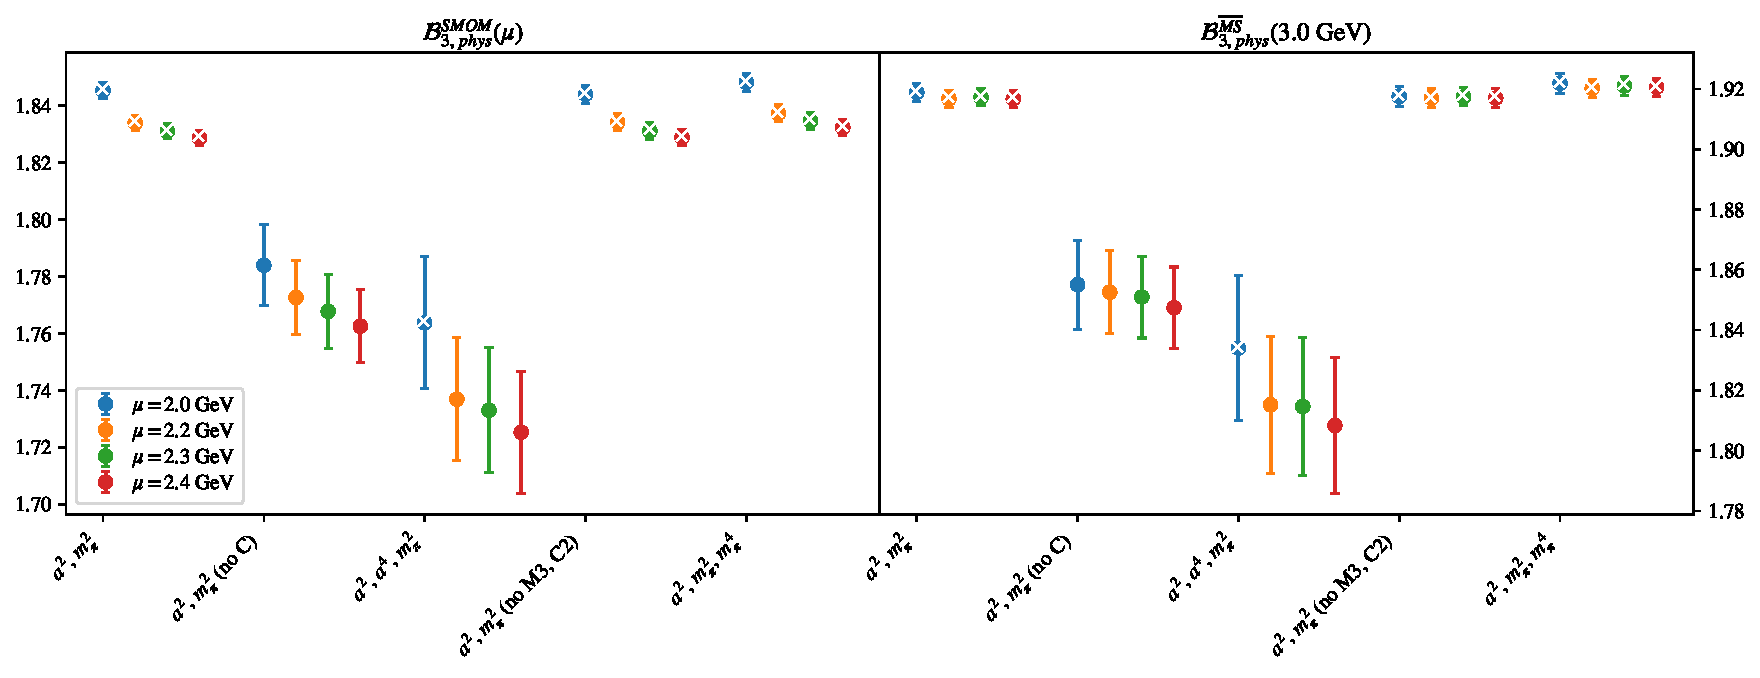
\includegraphics[page=1, width=1.1\textwidth]{SSmPP/NPR/fit_summary_bag.pdf}
\caption{$\mathcal{B}_{3}$\\(left) $\mathcal{B}_{phys}$ in RI/SMOM scheme from fit variations (fits with $p$-value $<0.05$ marked with ``$\times$"). \\(right) $\mathcal{B}_{phys}$ in $\overline{MS}$ computed using $\mathcal{B}^{\overline{MS}} = R^{\overline{MS}\leftarrow SMOM}(3.0)\sigma_{npt}(3.0,\mu) \mathcal{B}^{SMOM}(\mu)$.}
\end{figure}
\clearpage
\begin{figure}
\centering
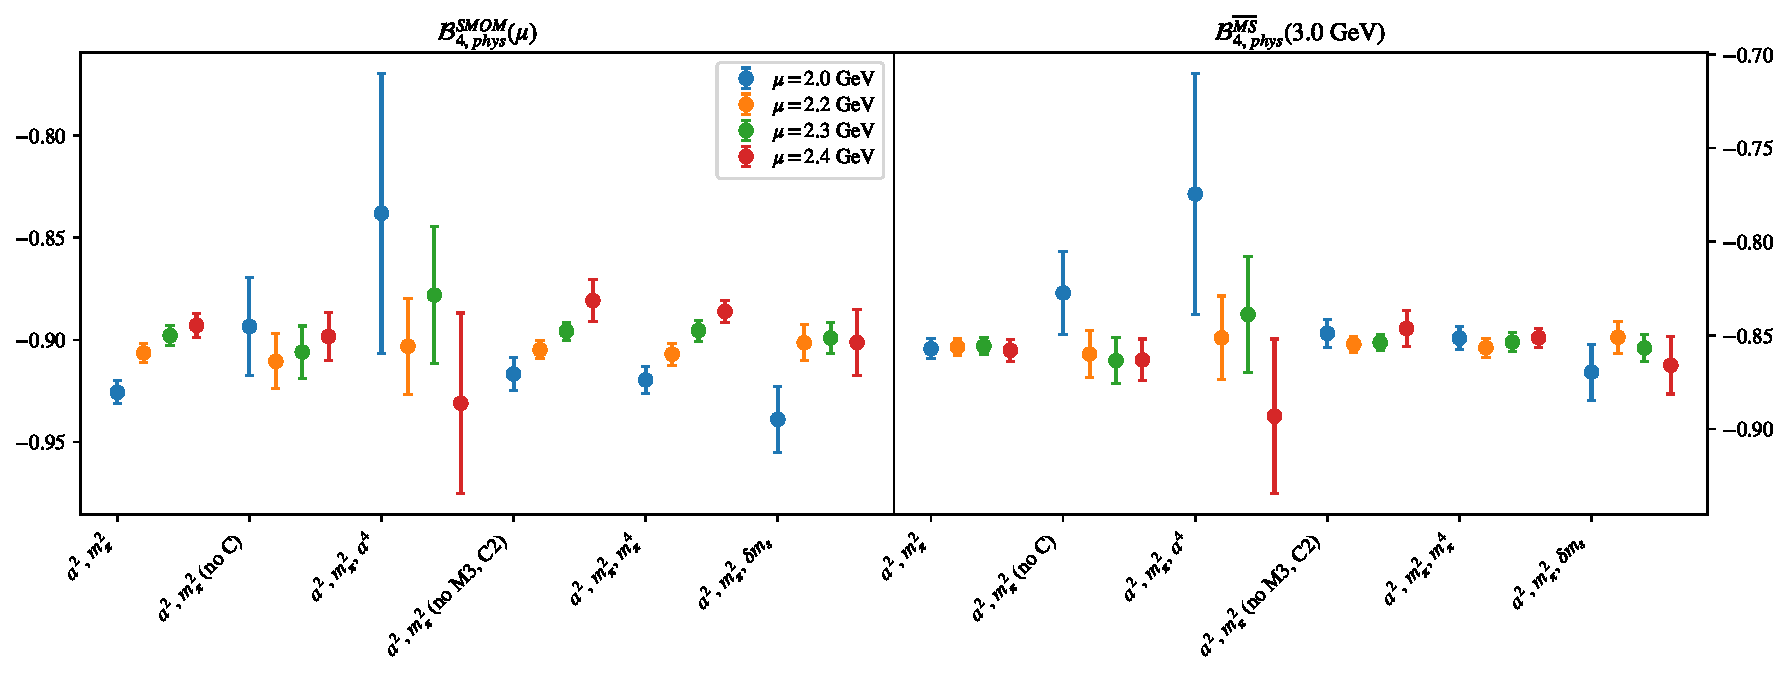
\includegraphics[page=1, width=1.1\textwidth]{SSpPP/NPR/fit_summary_bag.pdf}
\caption{$\mathcal{B}_{4}$\\(left) $\mathcal{B}_{phys}$ in RI/SMOM scheme from fit variations (fits with $p$-value $<0.05$ marked with ``$\times$"). \\(right) $\mathcal{B}_{phys}$ in $\overline{MS}$ computed using $\mathcal{B}^{\overline{MS}} = R^{\overline{MS}\leftarrow SMOM}(3.0)\sigma_{npt}(3.0,\mu) \mathcal{B}^{SMOM}(\mu)$.}
\end{figure}
\clearpage
\begin{figure}
\centering
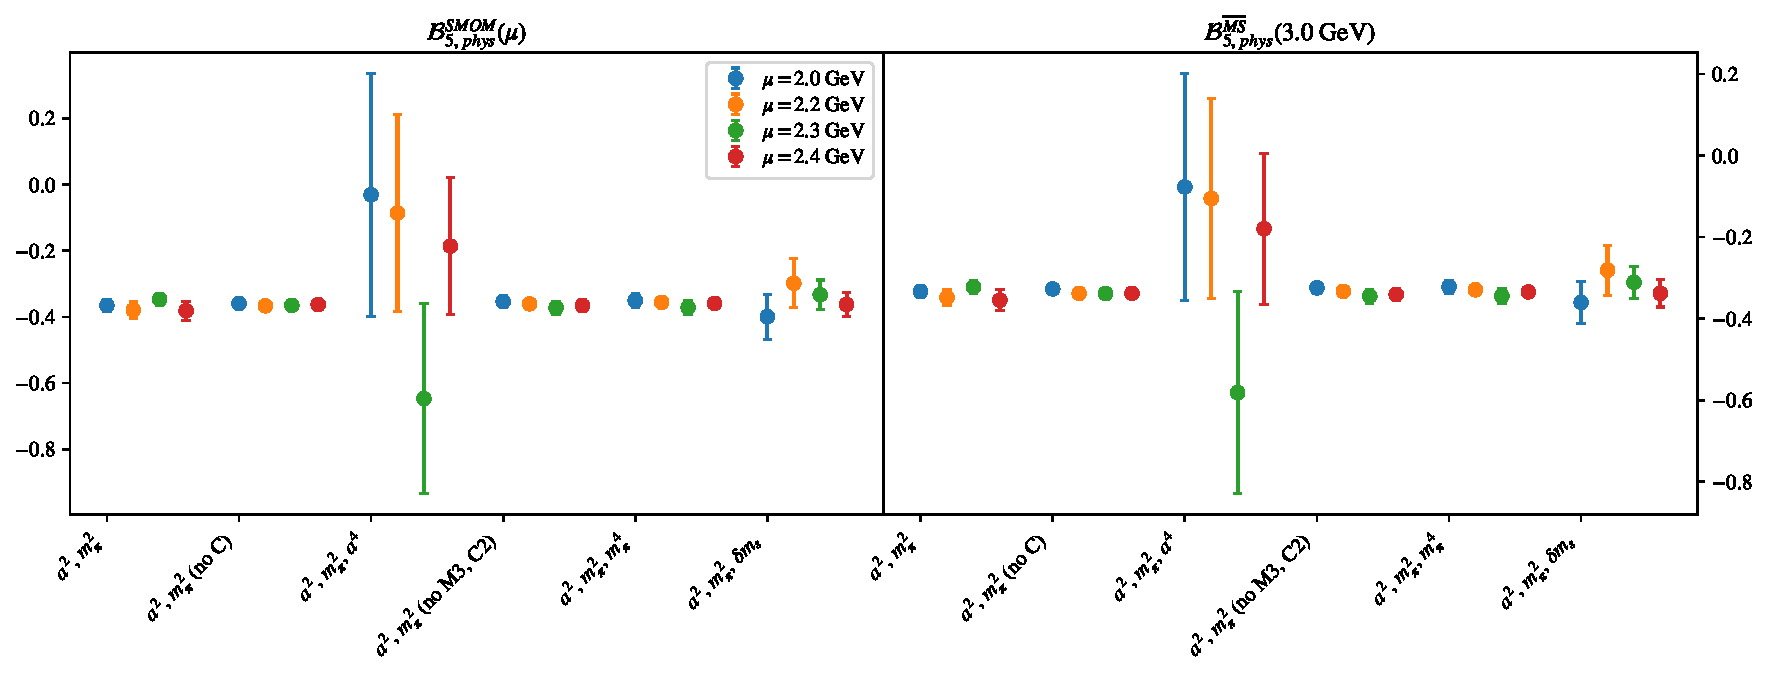
\includegraphics[page=1, width=1.1\textwidth]{TT/NPR/fit_summary_bag.pdf}
\caption{$\mathcal{B}_{5}$\\(left) $\mathcal{B}_{phys}$ in RI/SMOM scheme from fit variations (fits with $p$-value $<0.05$ marked with ``$\times$"). \\(right) $\mathcal{B}_{phys}$ in $\overline{MS}$ computed using $\mathcal{B}^{\overline{MS}} = R^{\overline{MS}\leftarrow SMOM}(3.0)\sigma_{npt}(3.0,\mu) \mathcal{B}^{SMOM}(\mu)$.}
\end{figure}
\clearpage
\section{$\mathcal{B}_1$}
\begin{table}[h!]
\begin{center}
\begin{tabular}{|c|c|c|c|c|c|}
\hline
$\mu$ (GeV) & $a^2$, $m_\pi^2$& $a^2$, $m_\pi^2$ (no C)& $a^2$, $a^4$, $m_\pi^2$& $a^2$, $m_\pi^2$ (no M3, C2)& $a^2$, $m_\pi^2$, $m_\pi^4$\\
\hline
2.0& \hyperlink{VVpAA/NPR/a2m2_20.pdf.1}{\textbf{1.4020(29)}: 2.323 (0.04)} & \hyperlink{VVpAA/NPR/a2m2noC_20.pdf.1}{\textbf{1.416(13)}: 0.863 (0.422)} & \hyperlink{VVpAA/NPR/a2a4m2_20.pdf.1}{\textbf{1.416(22)}: 2.677 (0.03)} & \hyperlink{VVpAA/NPR/a2m2mcut_20.pdf.1}{\textbf{1.4079(32)}: 0.271 (0.846)} & \hyperlink{VVpAA/NPR/a2m2m4_20.pdf.1}{\textbf{1.4076(34)}: 1.108 (0.351)}\\
2.2& \hyperlink{VVpAA/NPR/a2m2_22.pdf.1}{\textbf{1.3949(27)}: 2.653 (0.021)} & \hyperlink{VVpAA/NPR/a2m2noC_22.pdf.1}{\textbf{1.410(12)}: 1.143 (0.319)} & \hyperlink{VVpAA/NPR/a2a4m2_22.pdf.1}{\textbf{1.413(20)}: 3.064 (0.016)} & \hyperlink{VVpAA/NPR/a2m2mcut_22.pdf.1}{\textbf{1.4010(33)}: 0.398 (0.754)} & \hyperlink{VVpAA/NPR/a2m2m4_22.pdf.1}{\textbf{1.4008(33)}: 1.323 (0.259)}\\
2.3& \hyperlink{VVpAA/NPR/a2m2_23.pdf.1}{\textbf{1.3918(28)}: 2.676 (0.02)} & \hyperlink{VVpAA/NPR/a2m2noC_23.pdf.1}{\textbf{1.408(12)}: 1.177 (0.308)} & \hyperlink{VVpAA/NPR/a2a4m2_23.pdf.1}{\textbf{1.412(20)}: 2.994 (0.018)} & \hyperlink{VVpAA/NPR/a2m2mcut_23.pdf.1}{\textbf{1.3980(33)}: 0.448 (0.719)} & \hyperlink{VVpAA/NPR/a2m2m4_23.pdf.1}{\textbf{1.3978(33)}: 1.369 (0.242)}\\
2.4& \hyperlink{VVpAA/NPR/a2m2_24.pdf.1}{\textbf{1.3890(28)}: 2.726 (0.018)} & \hyperlink{VVpAA/NPR/a2m2noC_24.pdf.1}{\textbf{1.405(12)}: 1.211 (0.298)} & \hyperlink{VVpAA/NPR/a2a4m2_24.pdf.1}{\textbf{1.410(20)}: 3.126 (0.014)} & \hyperlink{VVpAA/NPR/a2m2mcut_24.pdf.1}{\textbf{1.3953(34)}: 0.45 (0.718)} & \hyperlink{VVpAA/NPR/a2m2m4_24.pdf.1}{\textbf{1.3951(34)}: 1.364 (0.244)}\\
\hline
\end{tabular}
\caption{Physical point value from chiral and continuum extrapolation at renormalisation scale $\mu$. Entries are \textbf{value(error)}: $\chi^2/\text{DOF}$ ($p$-value).}
\end{center}
\end{table}
\begin{table}[h!]
\begin{center}
\begin{tabular}{|c c|c|c|c|c|c|}
\hline
$\mu$ (GeV) &  & $a^2$, $m_\pi^2$& $a^2$, $m_\pi^2$ (no C)& $a^2$, $a^4$, $m_\pi^2$& $a^2$, $m_\pi^2$ (no M3, C2)& $a^2$, $m_\pi^2$, $m_\pi^4$\\
\hline
\multirow{2}{0.5in}{2.0} & $\alpha$ & 0.0986(76)& 0.047(55)& 0.007& 0.0843(84)& 0.0856(85)\\
 & $\beta$ & 0.00279(17)& 0.00223(27)& 0.00278(18)& 0.00200(29)& 0.00029(89)\\
\hline
\multirow{2}{0.5in}{2.2} & $\alpha$ & 0.1018(71)& 0.042(51)& -0.02& 0.0870(85)& 0.0882(83)\\
 & $\beta$ & 0.00275(16)& 0.00220(27)& 0.00277(16)& 0.00193(29)& 0.00017(89)\\
\hline
\multirow{2}{0.5in}{2.3} & $\alpha$ & 0.1028(75)& 0.039(51)& -0.034& 0.0878(87)& 0.0890(83)\\
 & $\beta$ & 0.00275(16)& 0.00221(27)& 0.00276(17)& 0.00191(29)& 0.00016(89)\\
\hline
\multirow{2}{0.5in}{2.4} & $\alpha$ & 0.1033(74)& 0.040(51)& -0.035& 0.0881(87)& 0.0892(85)\\
 & $\beta$ & 0.00276(16)& 0.00221(27)& 0.00278(16)& 0.00191(30)& 0.00015(89)\\
\hline
\end{tabular}
\caption{Fit values of coefficients in $Q = Q_{phys} + \mathbf{\alpha} a^2 + \mathbf{\beta}\left(\frac{m_\pi^2}{f_\pi^2}-\frac{m_{\pi,PDG}^2}{f_\pi^2}\right) + \ldots$.}
\end{center}
\end{table}
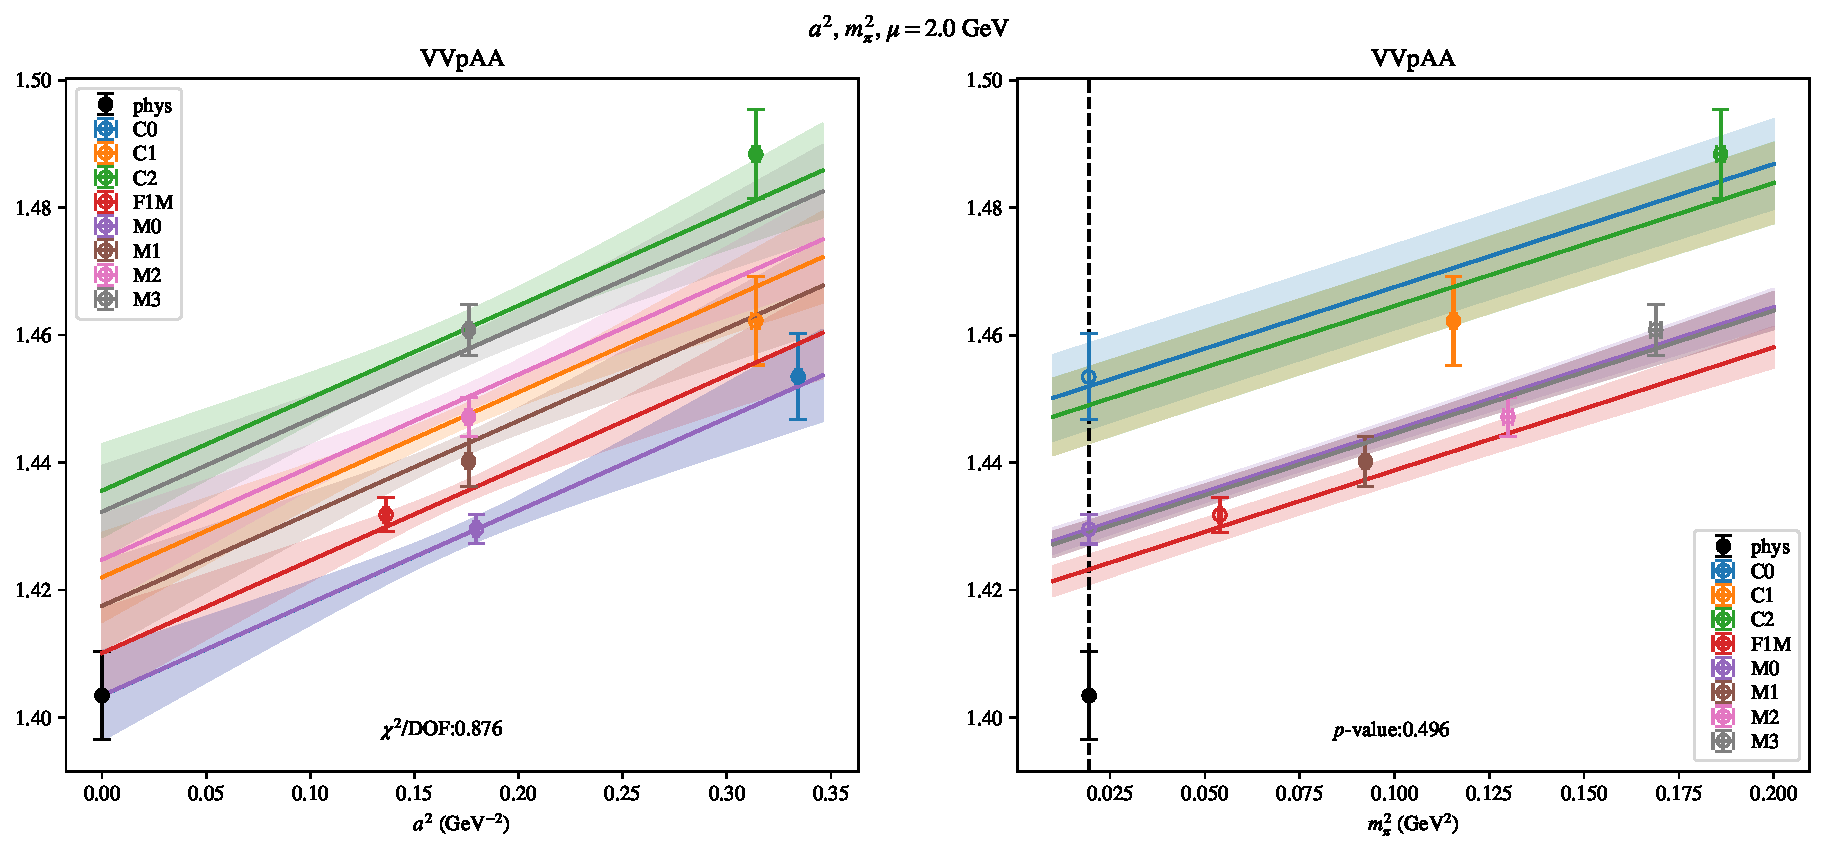
\includepdf[link, pages=-]{VVpAA/NPR/a2m2_20.pdf}
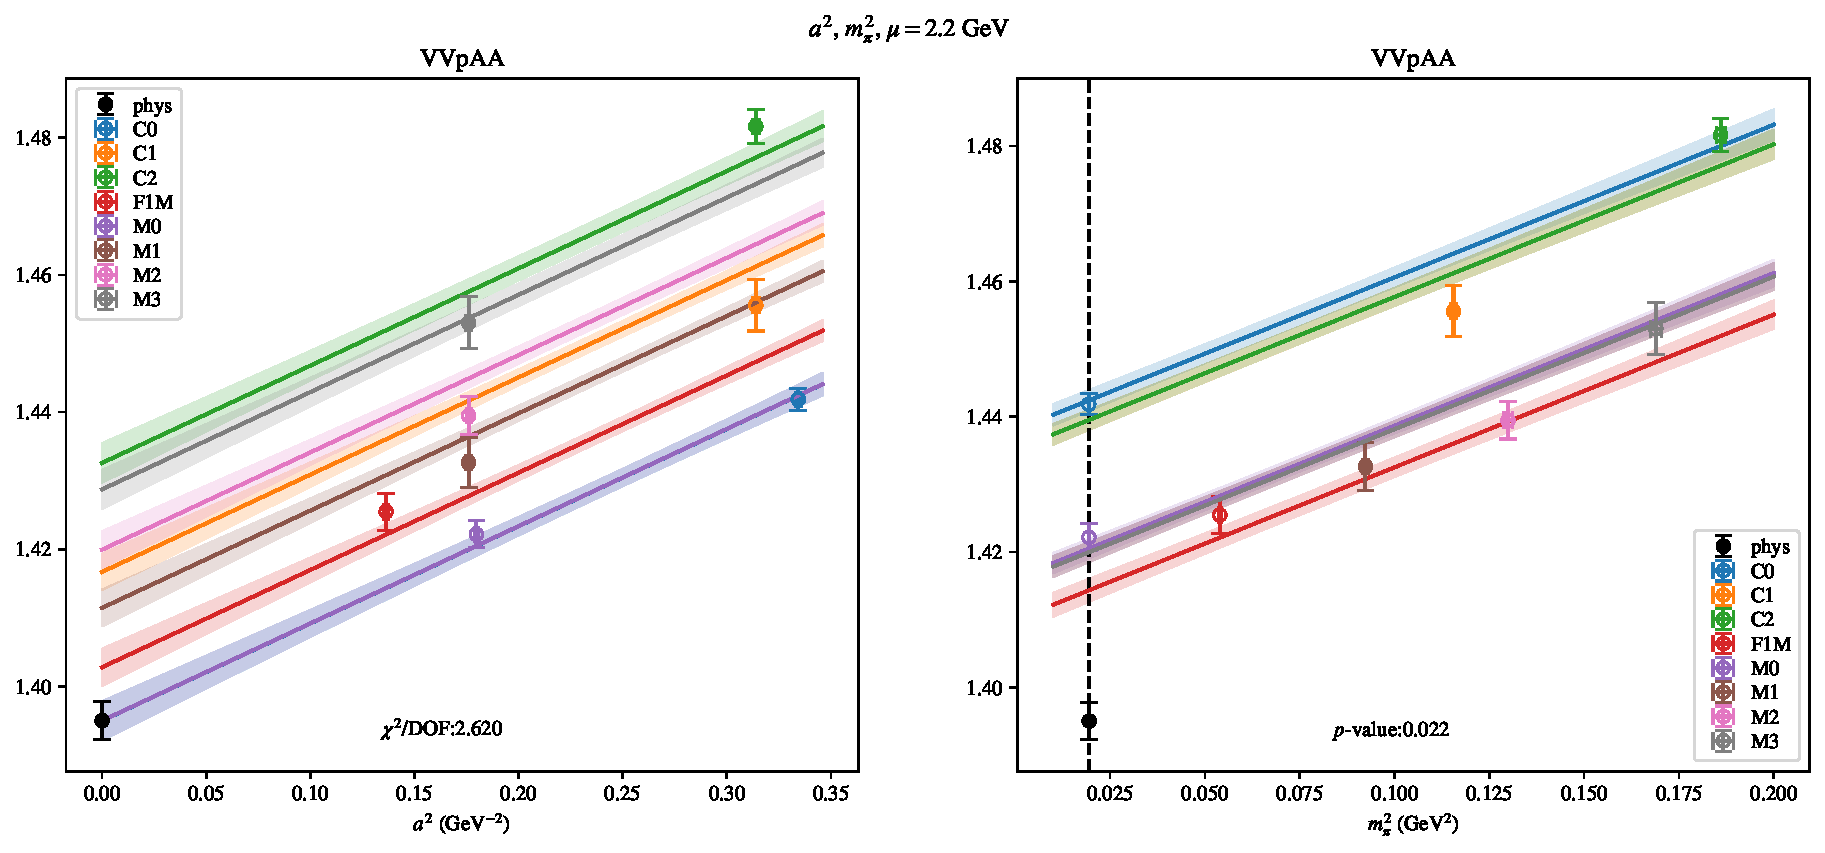
\includepdf[link, pages=-]{VVpAA/NPR/a2m2_22.pdf}
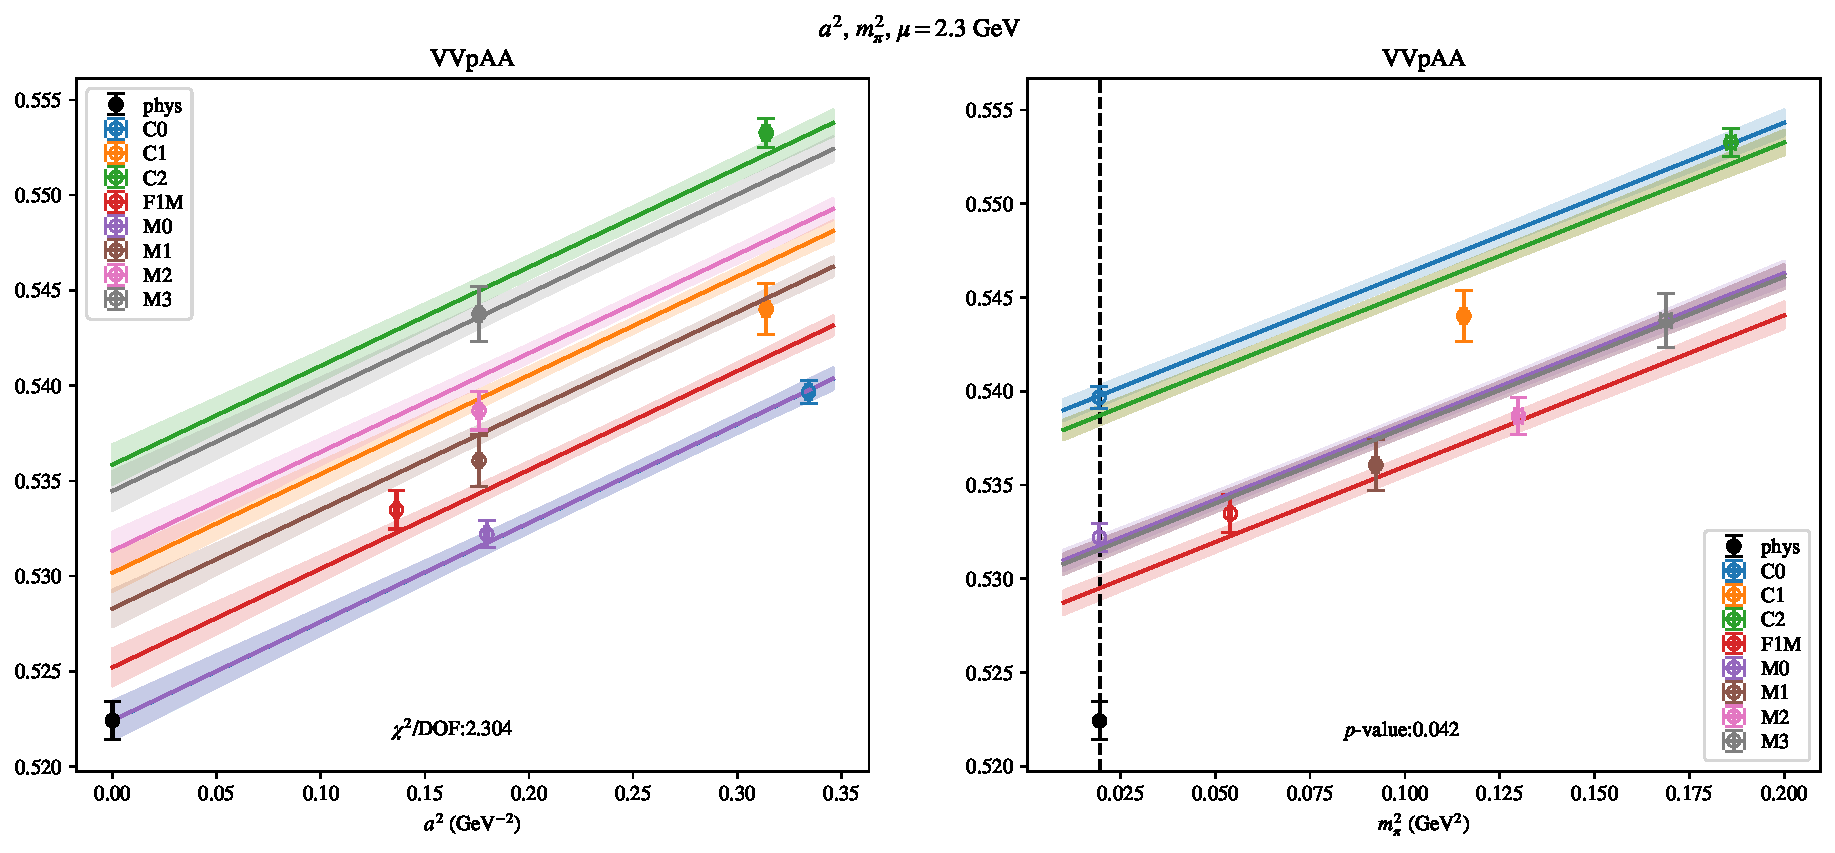
\includepdf[link, pages=-]{VVpAA/NPR/a2m2_23.pdf}
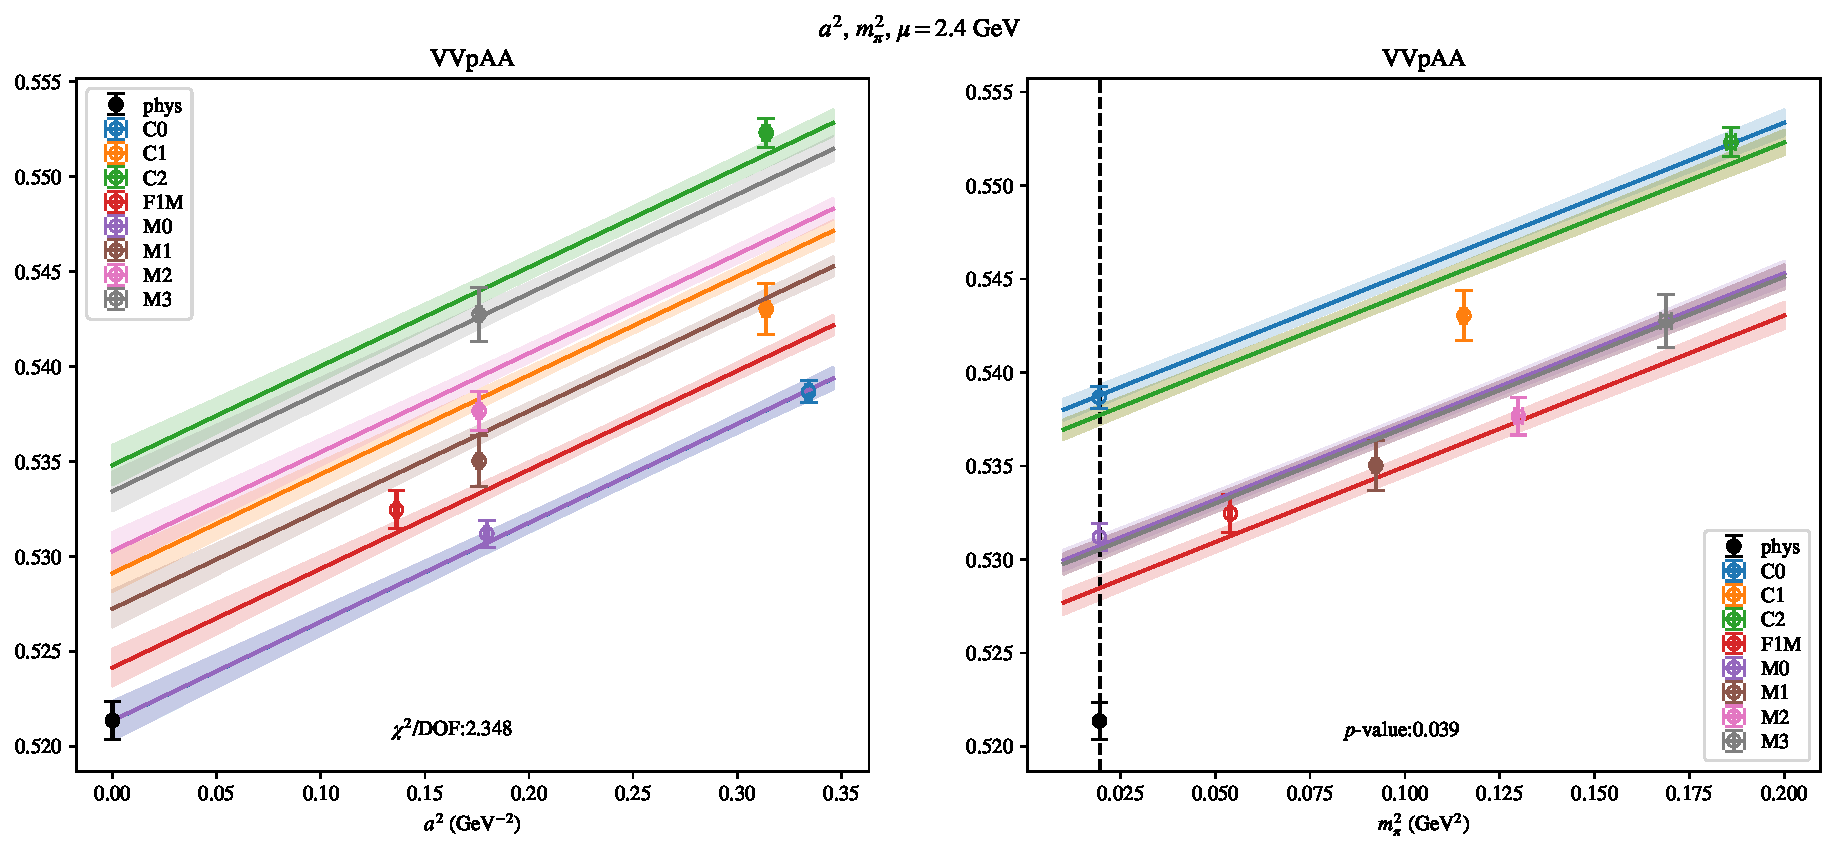
\includepdf[link, pages=-]{VVpAA/NPR/a2m2_24.pdf}
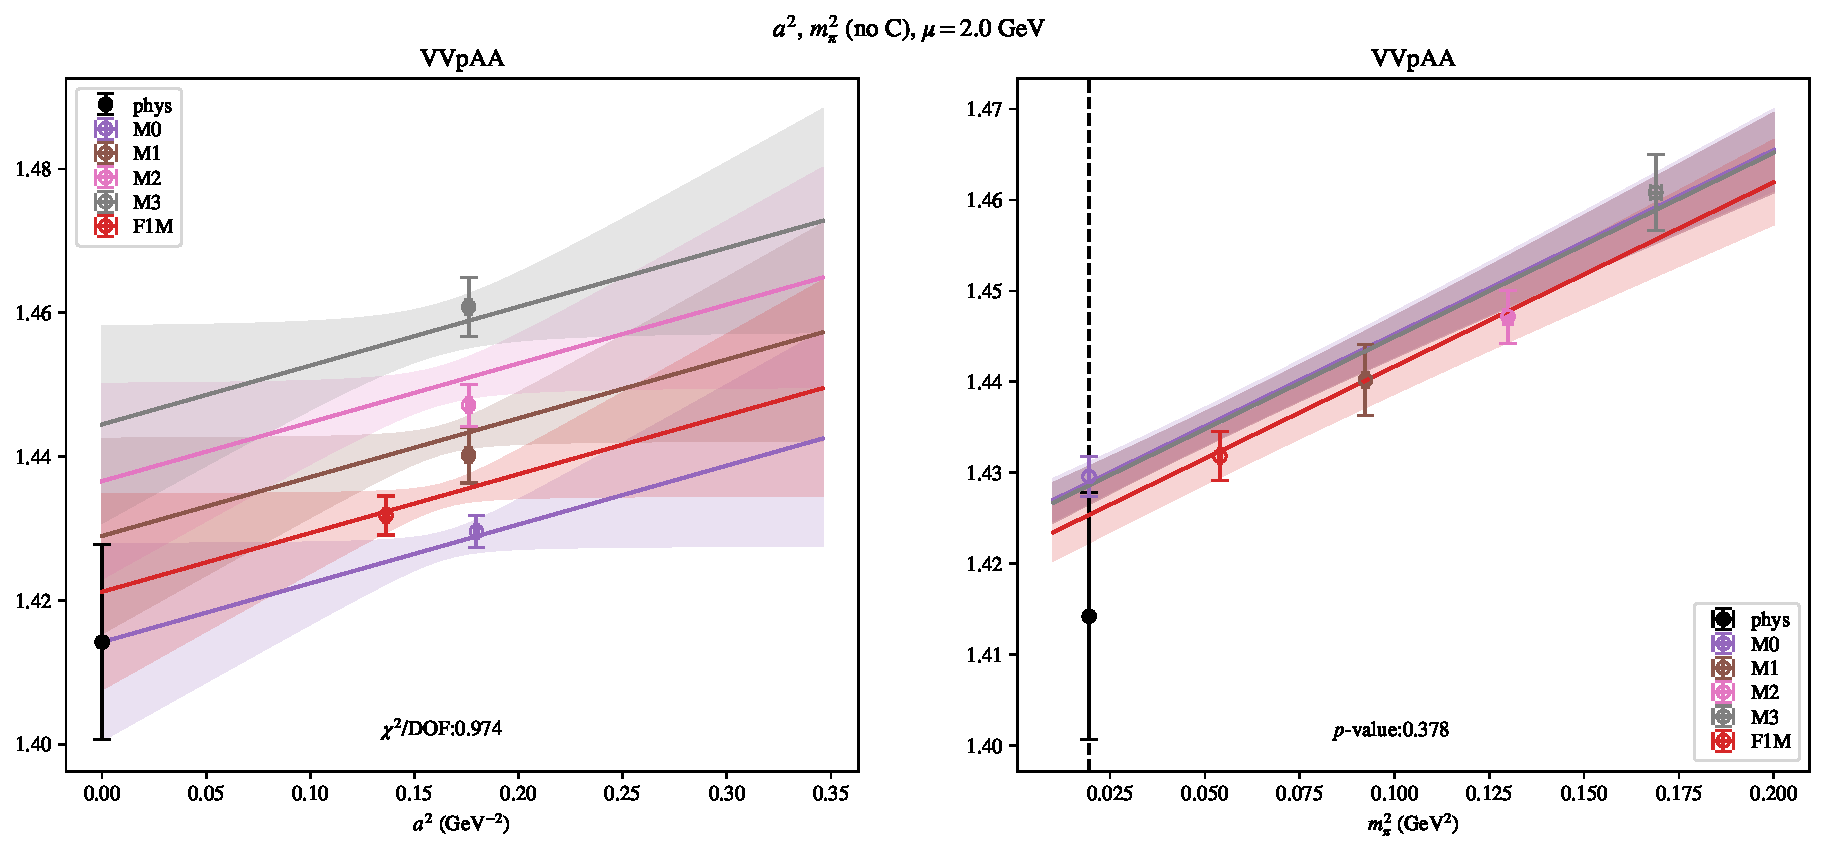
\includepdf[link, pages=-]{VVpAA/NPR/a2m2noC_20.pdf}
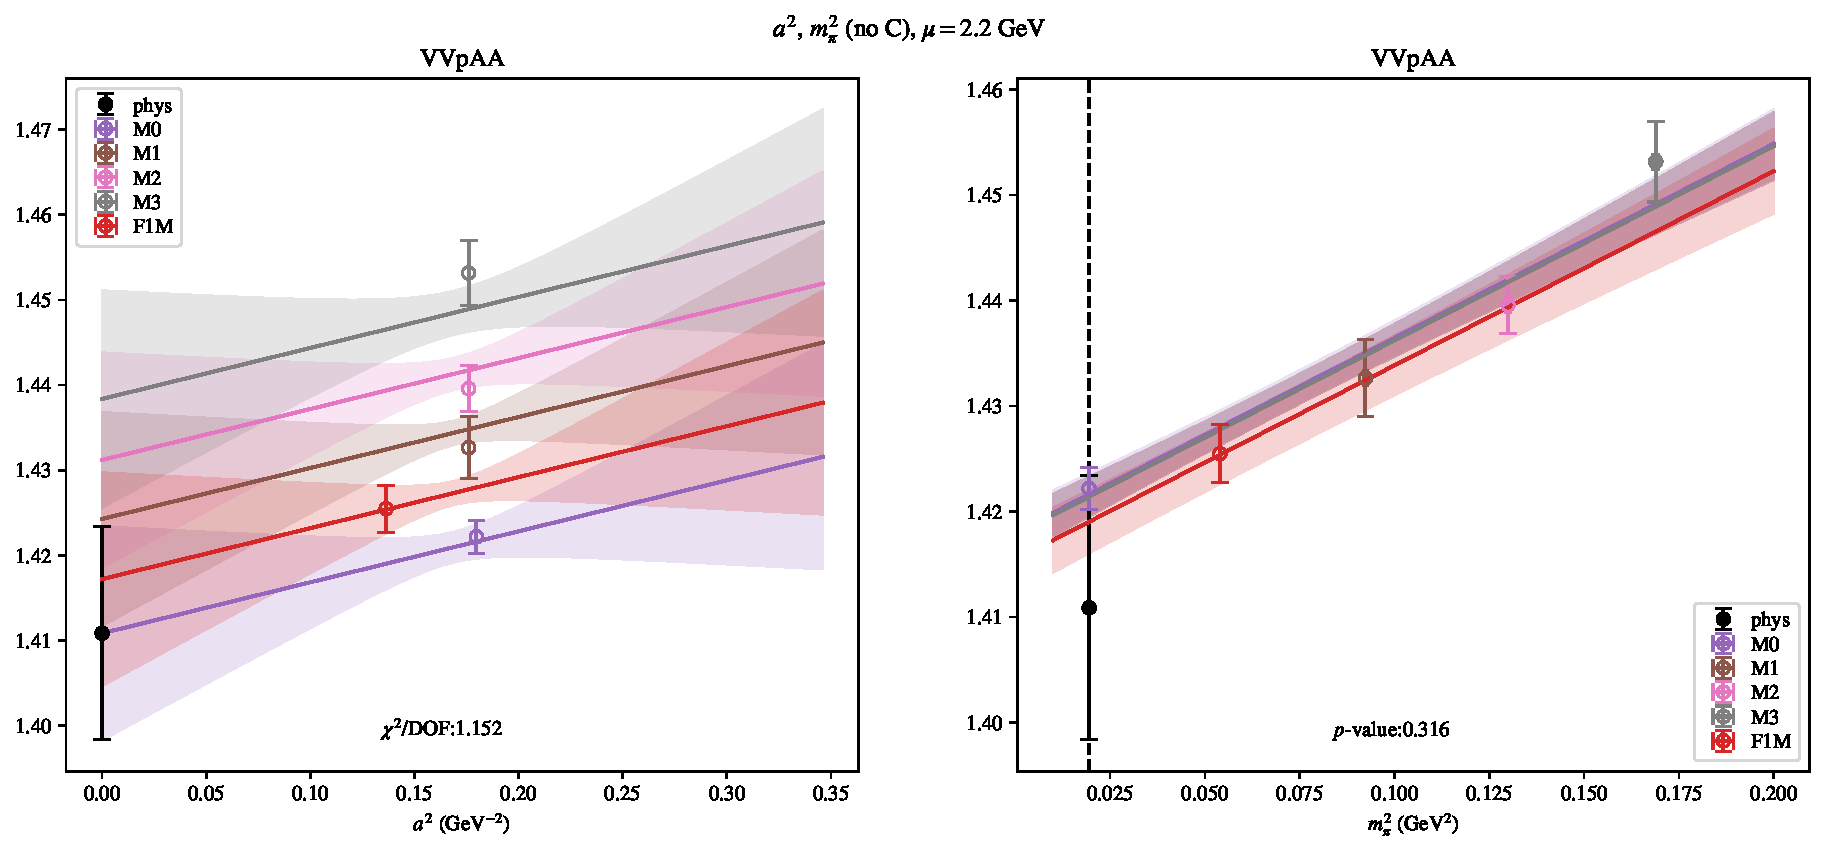
\includepdf[link, pages=-]{VVpAA/NPR/a2m2noC_22.pdf}
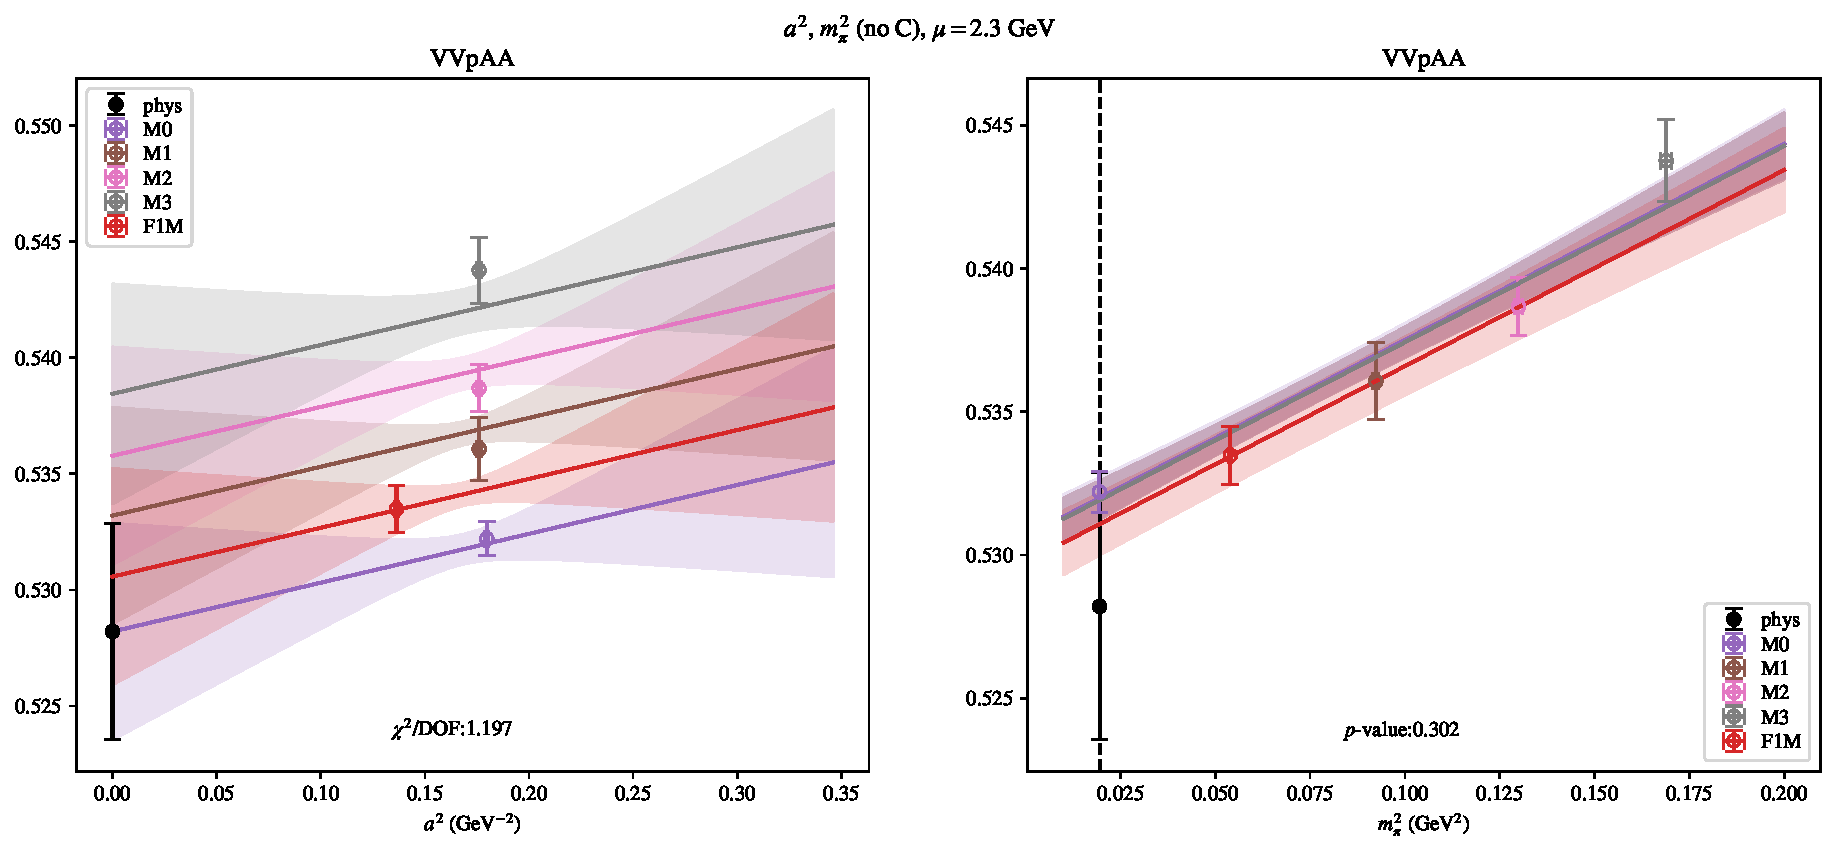
\includepdf[link, pages=-]{VVpAA/NPR/a2m2noC_23.pdf}
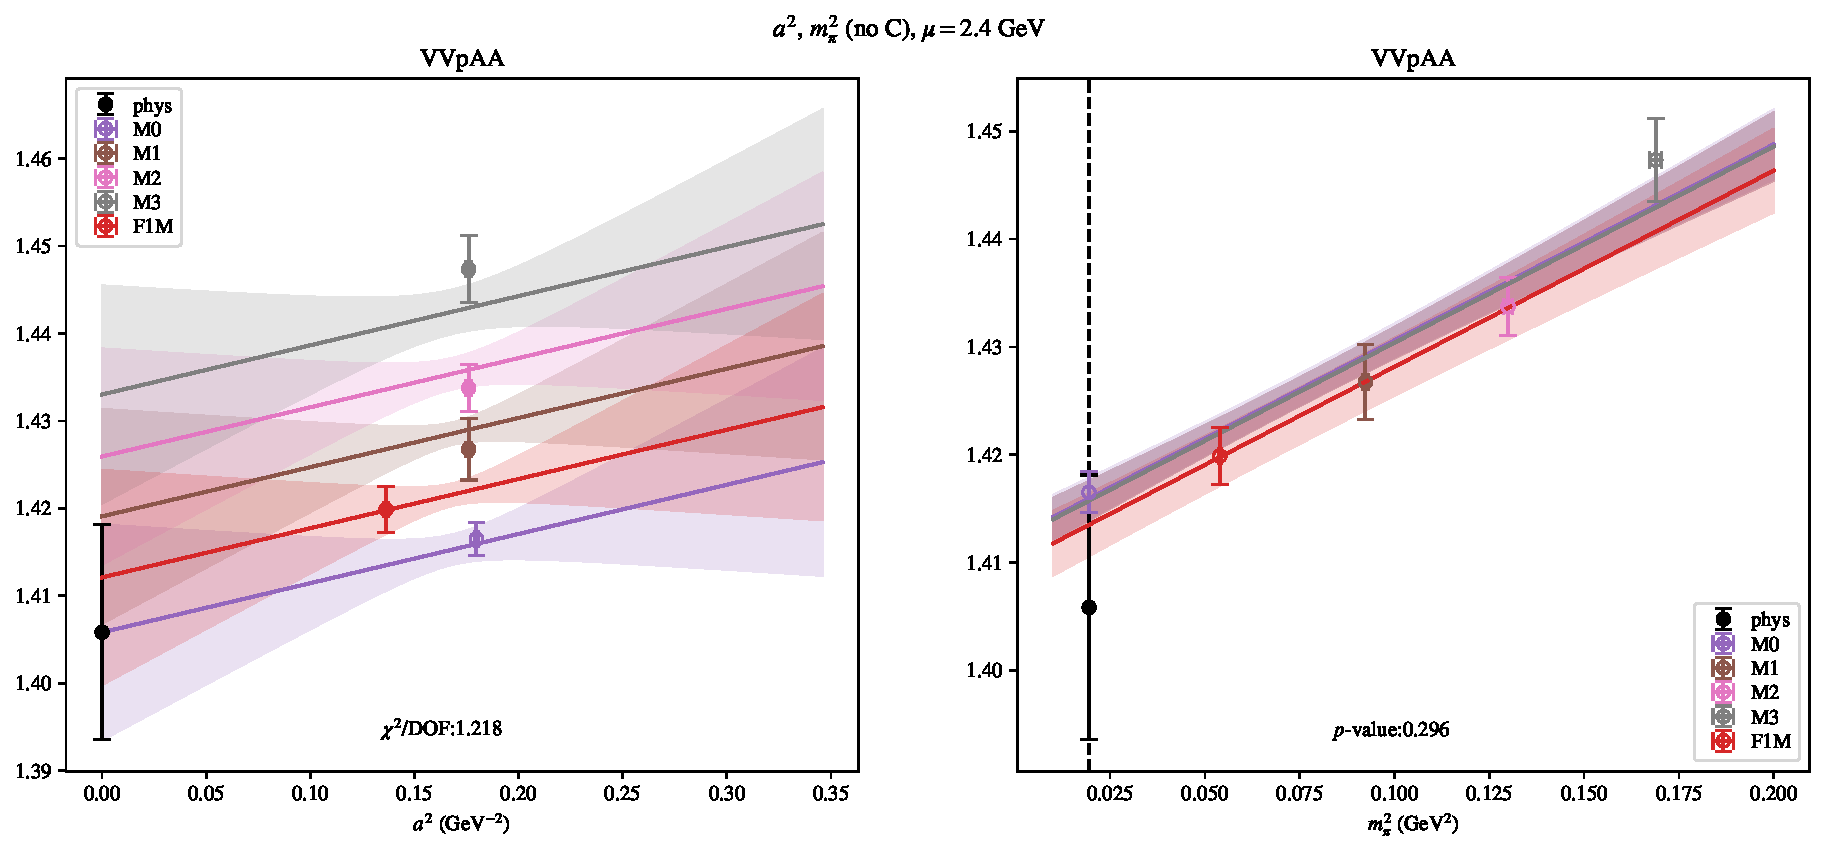
\includepdf[link, pages=-]{VVpAA/NPR/a2m2noC_24.pdf}
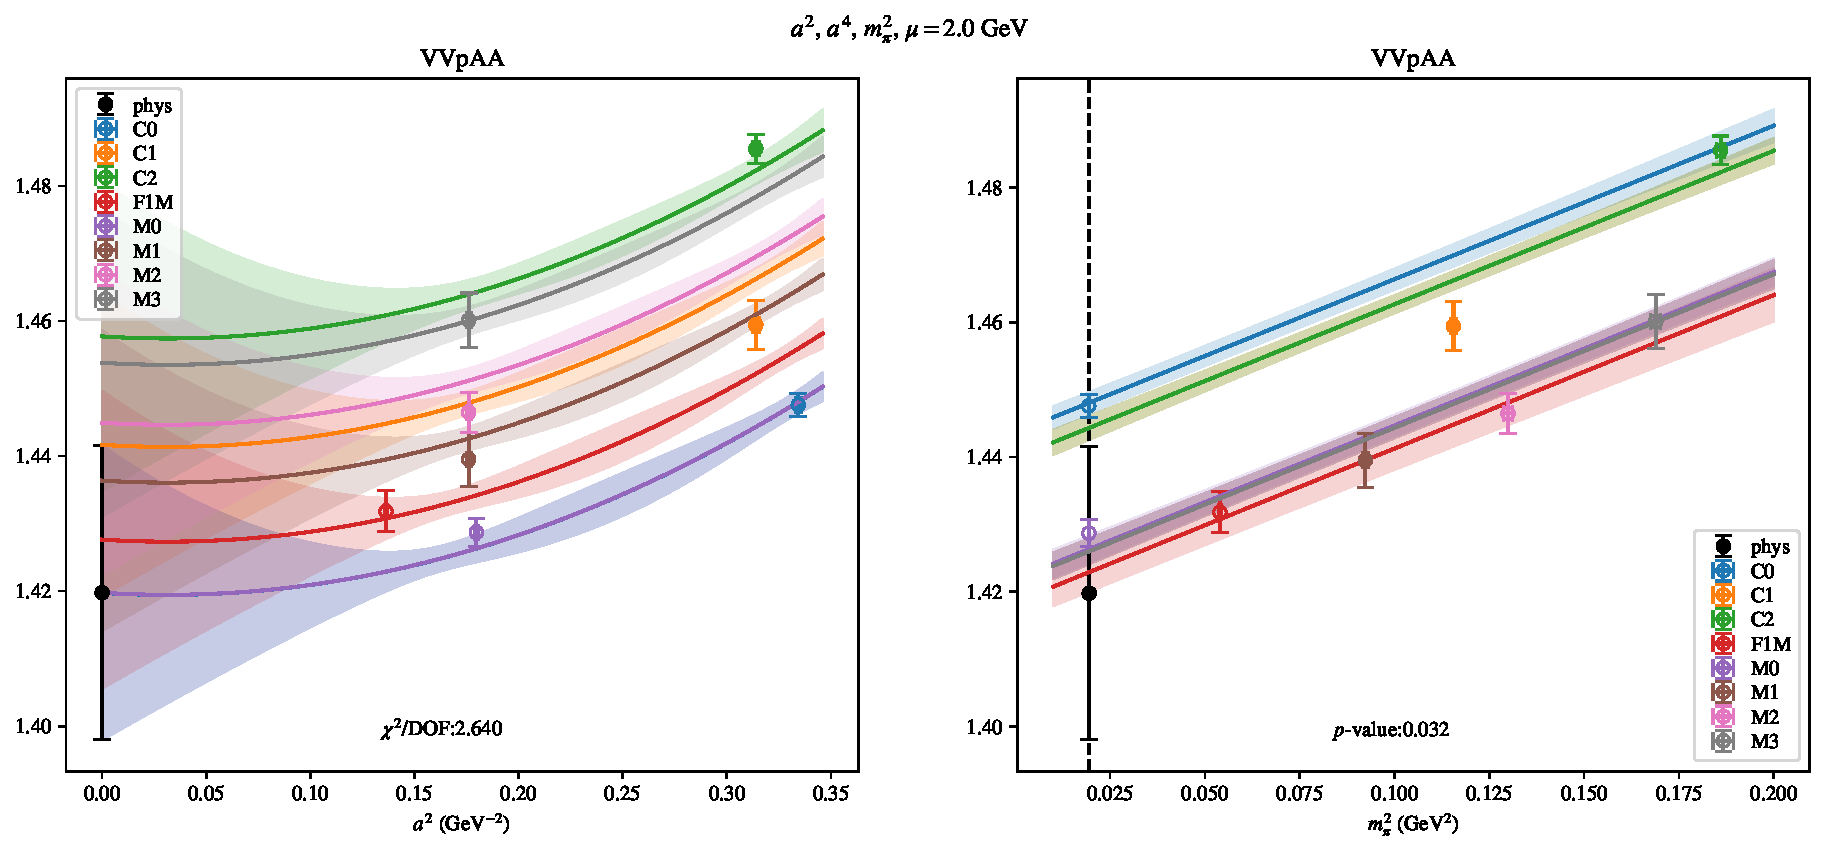
\includepdf[link, pages=-]{VVpAA/NPR/a2a4m2_20.pdf}
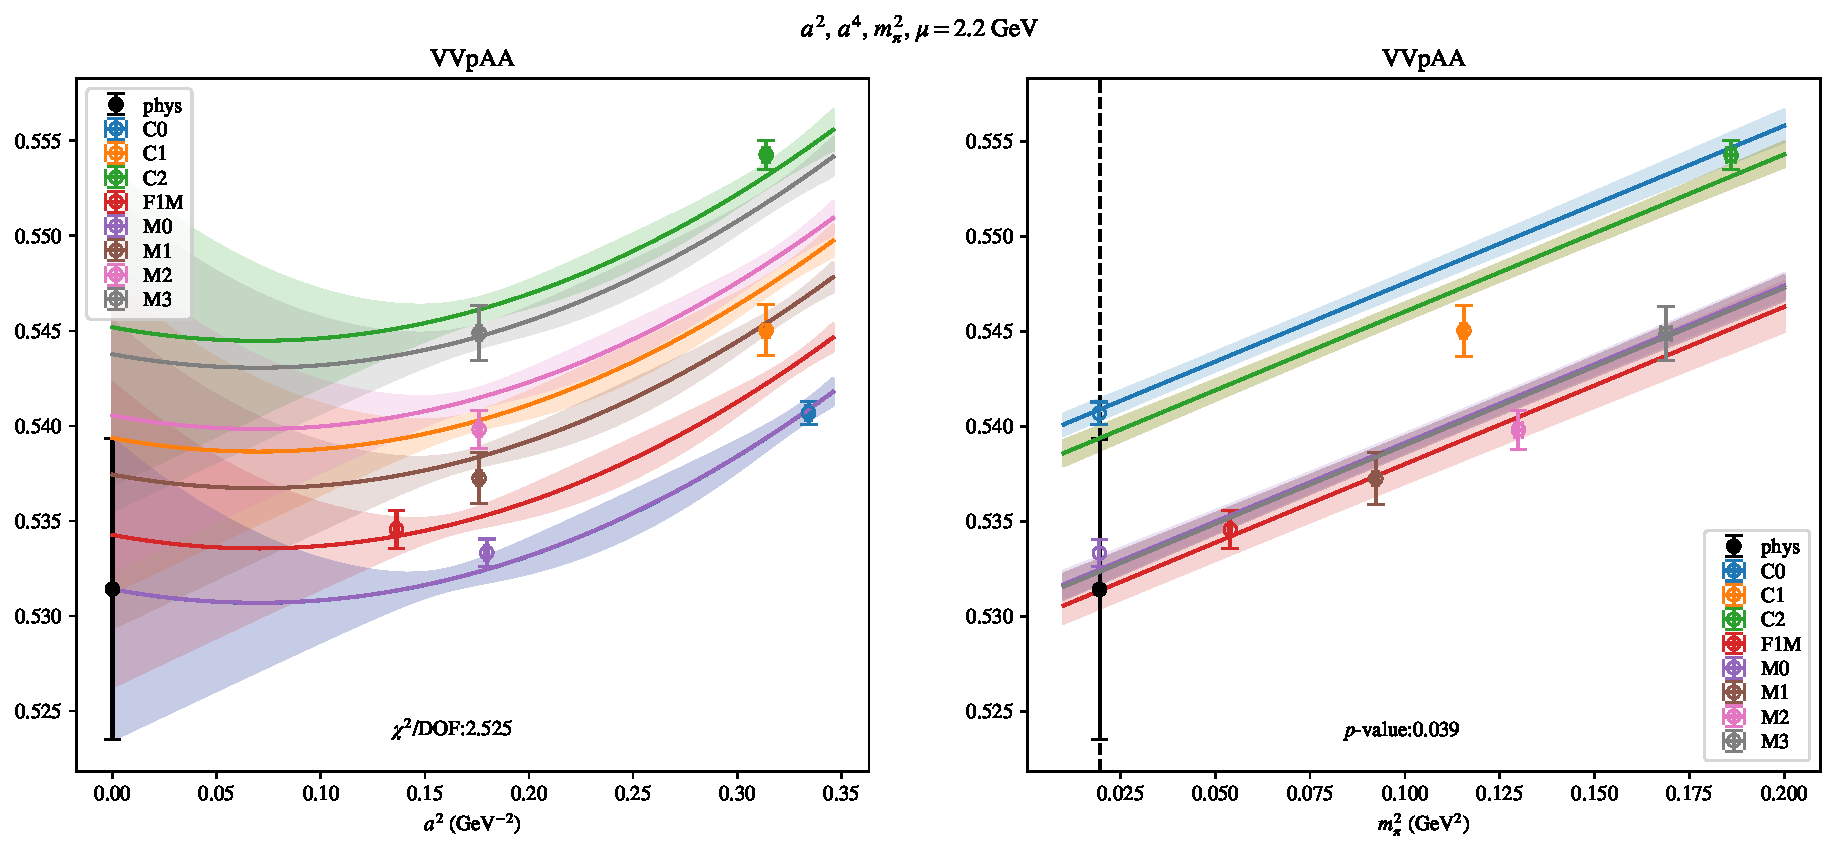
\includepdf[link, pages=-]{VVpAA/NPR/a2a4m2_22.pdf}
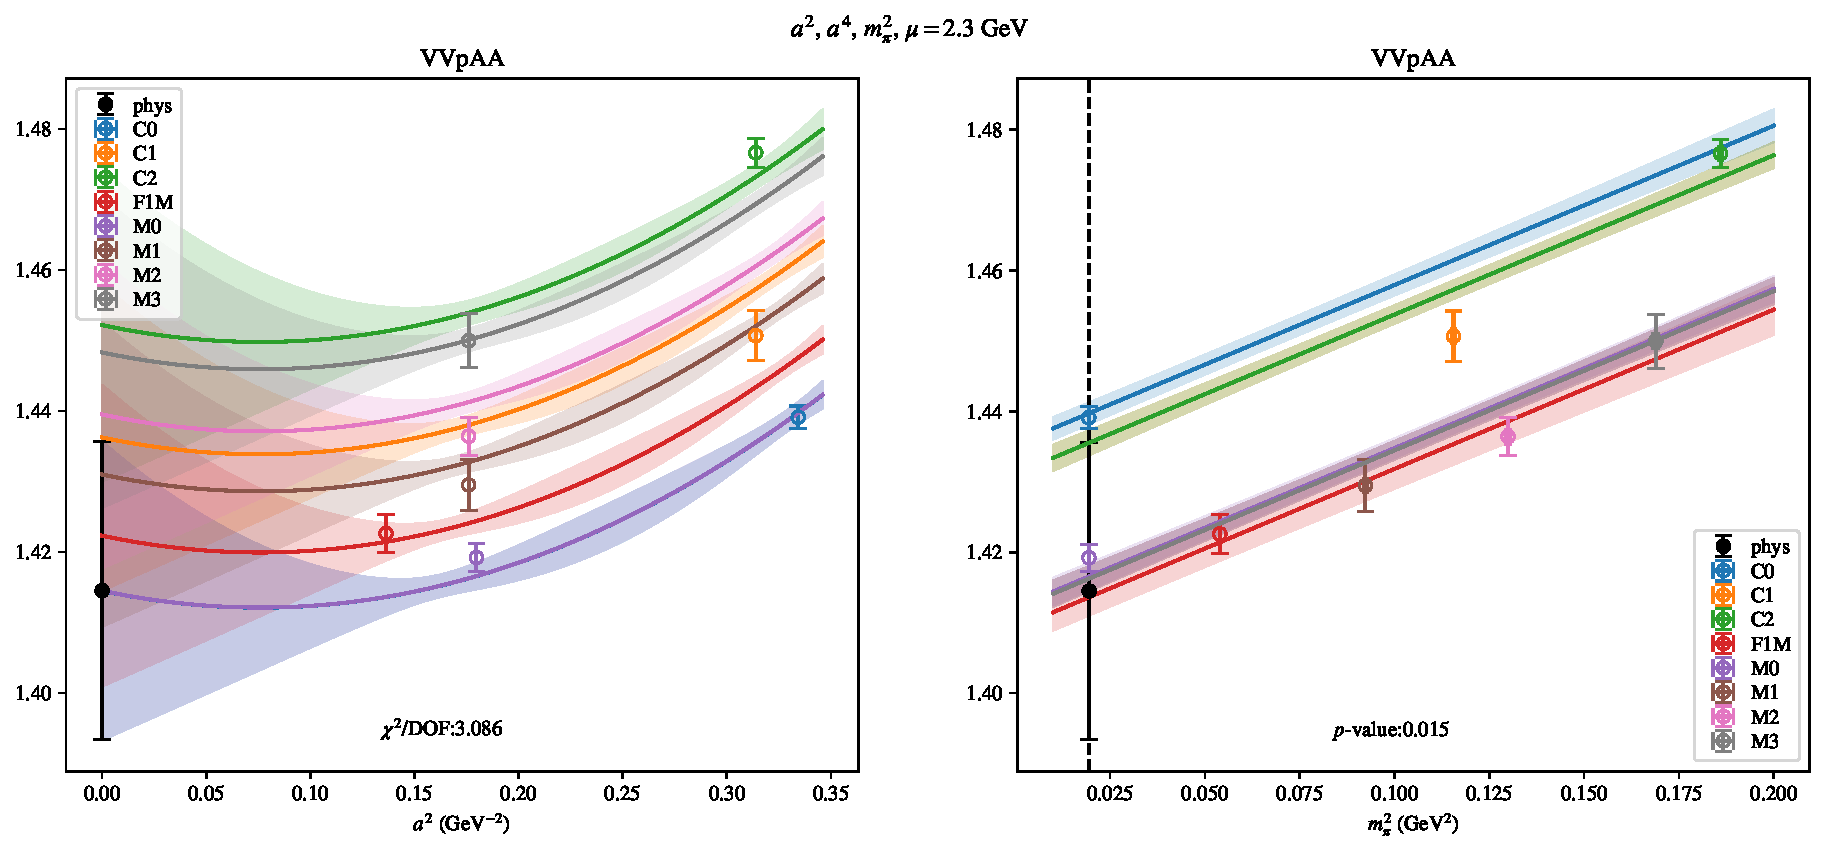
\includepdf[link, pages=-]{VVpAA/NPR/a2a4m2_23.pdf}
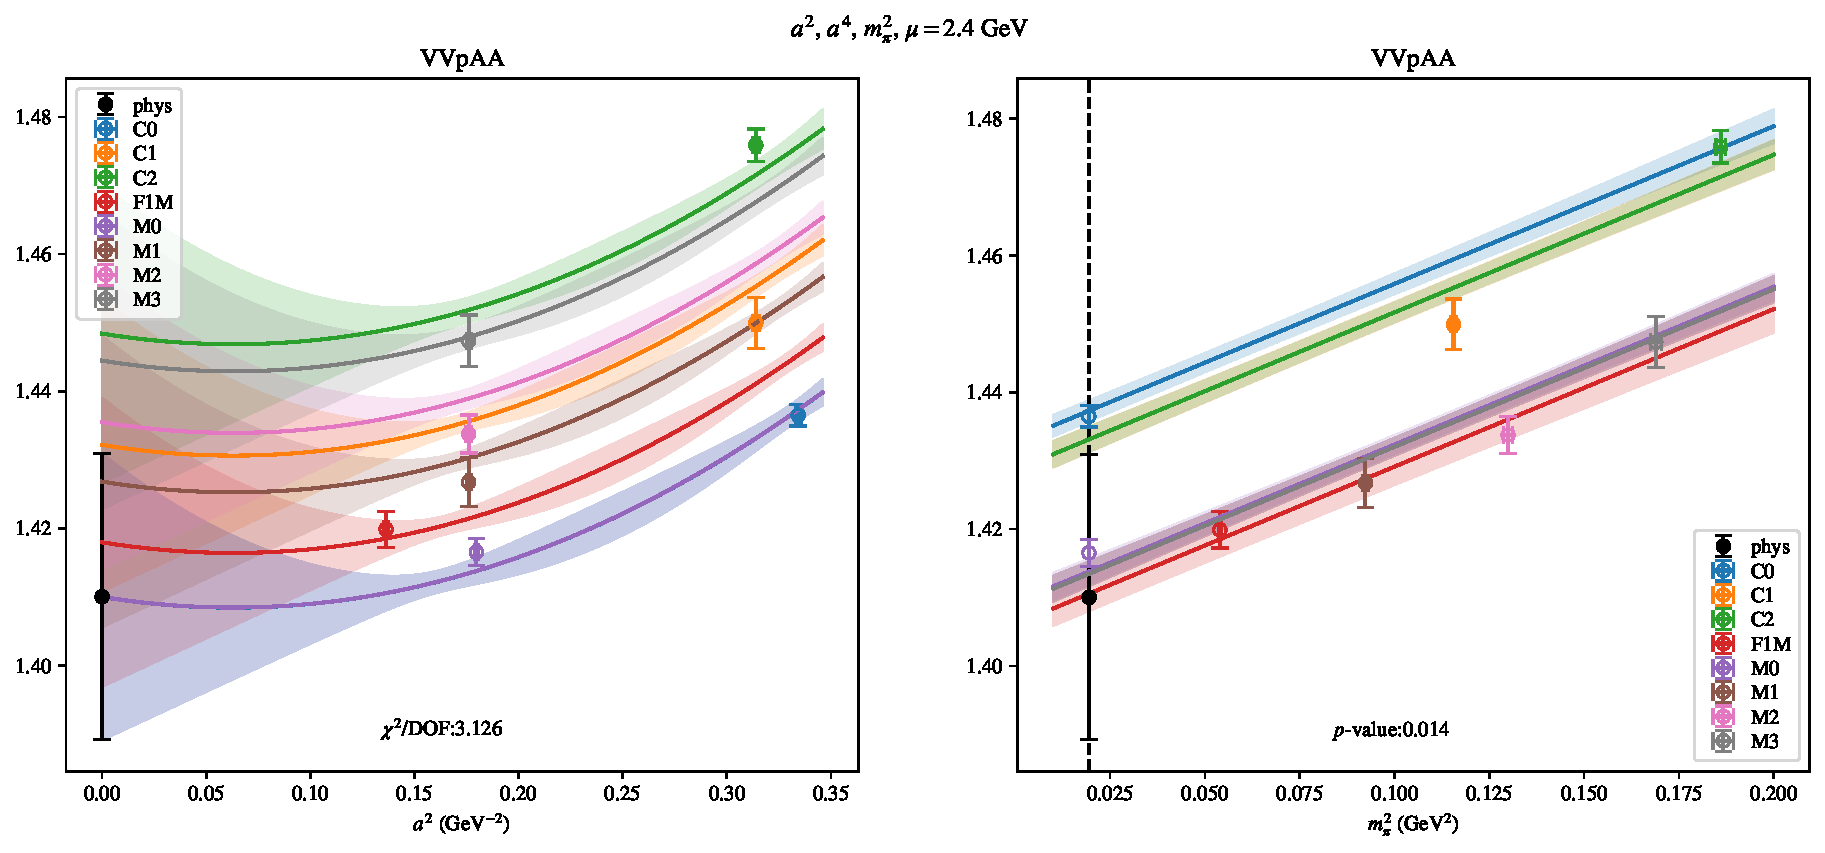
\includepdf[link, pages=-]{VVpAA/NPR/a2a4m2_24.pdf}
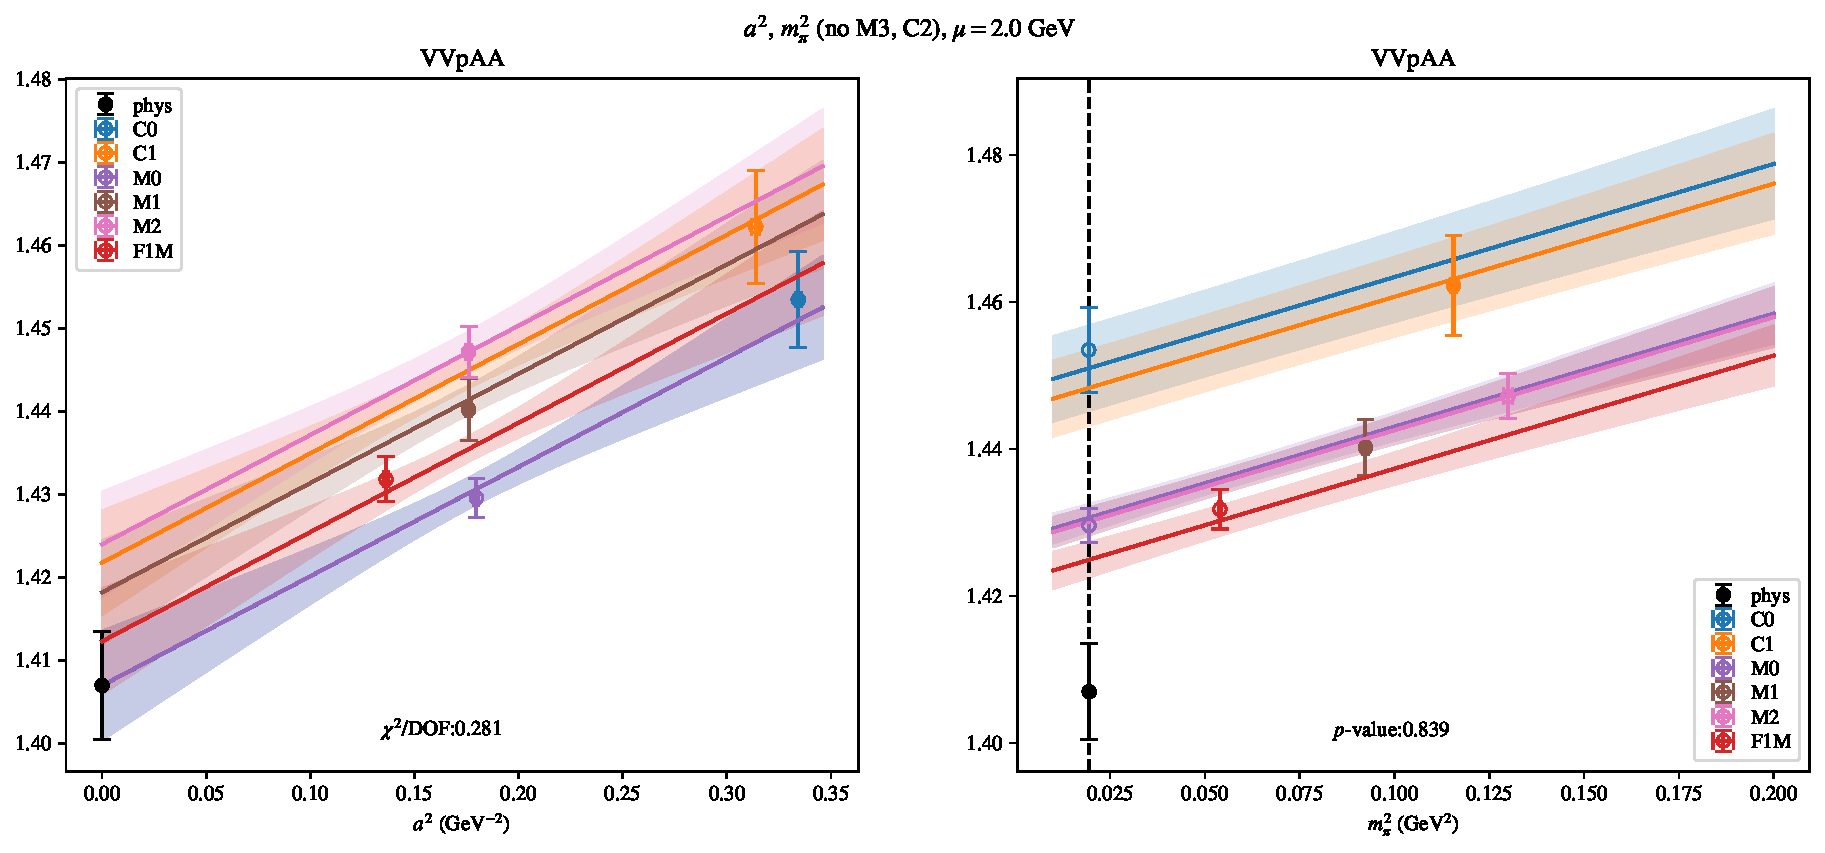
\includepdf[link, pages=-]{VVpAA/NPR/a2m2mcut_20.pdf}
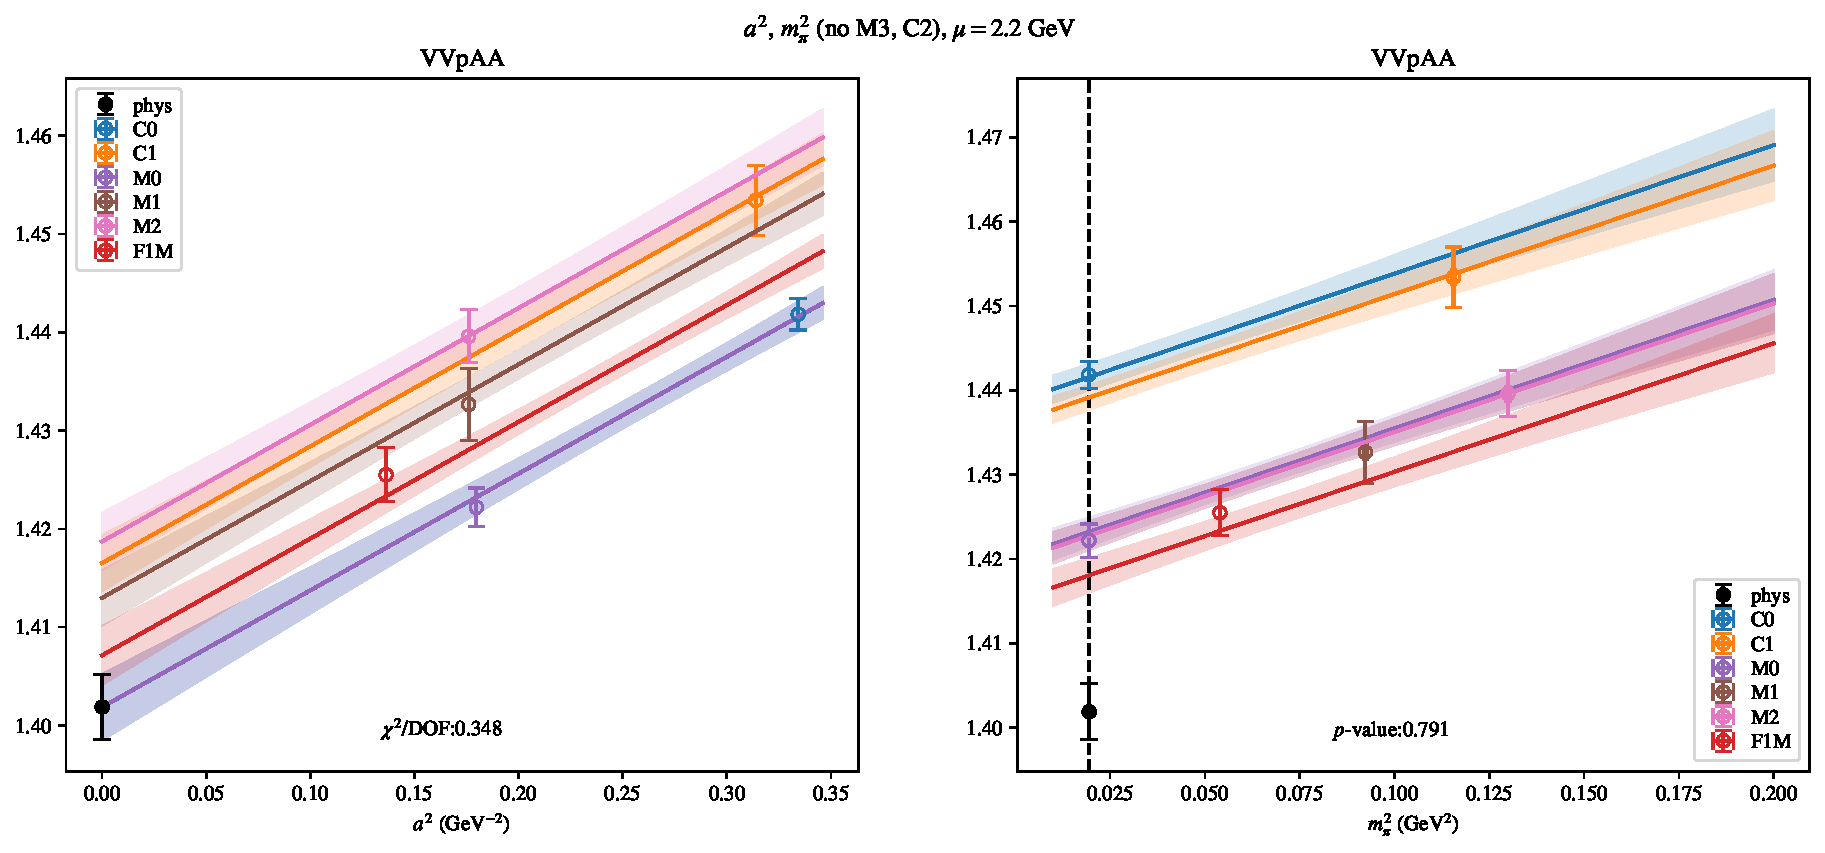
\includepdf[link, pages=-]{VVpAA/NPR/a2m2mcut_22.pdf}
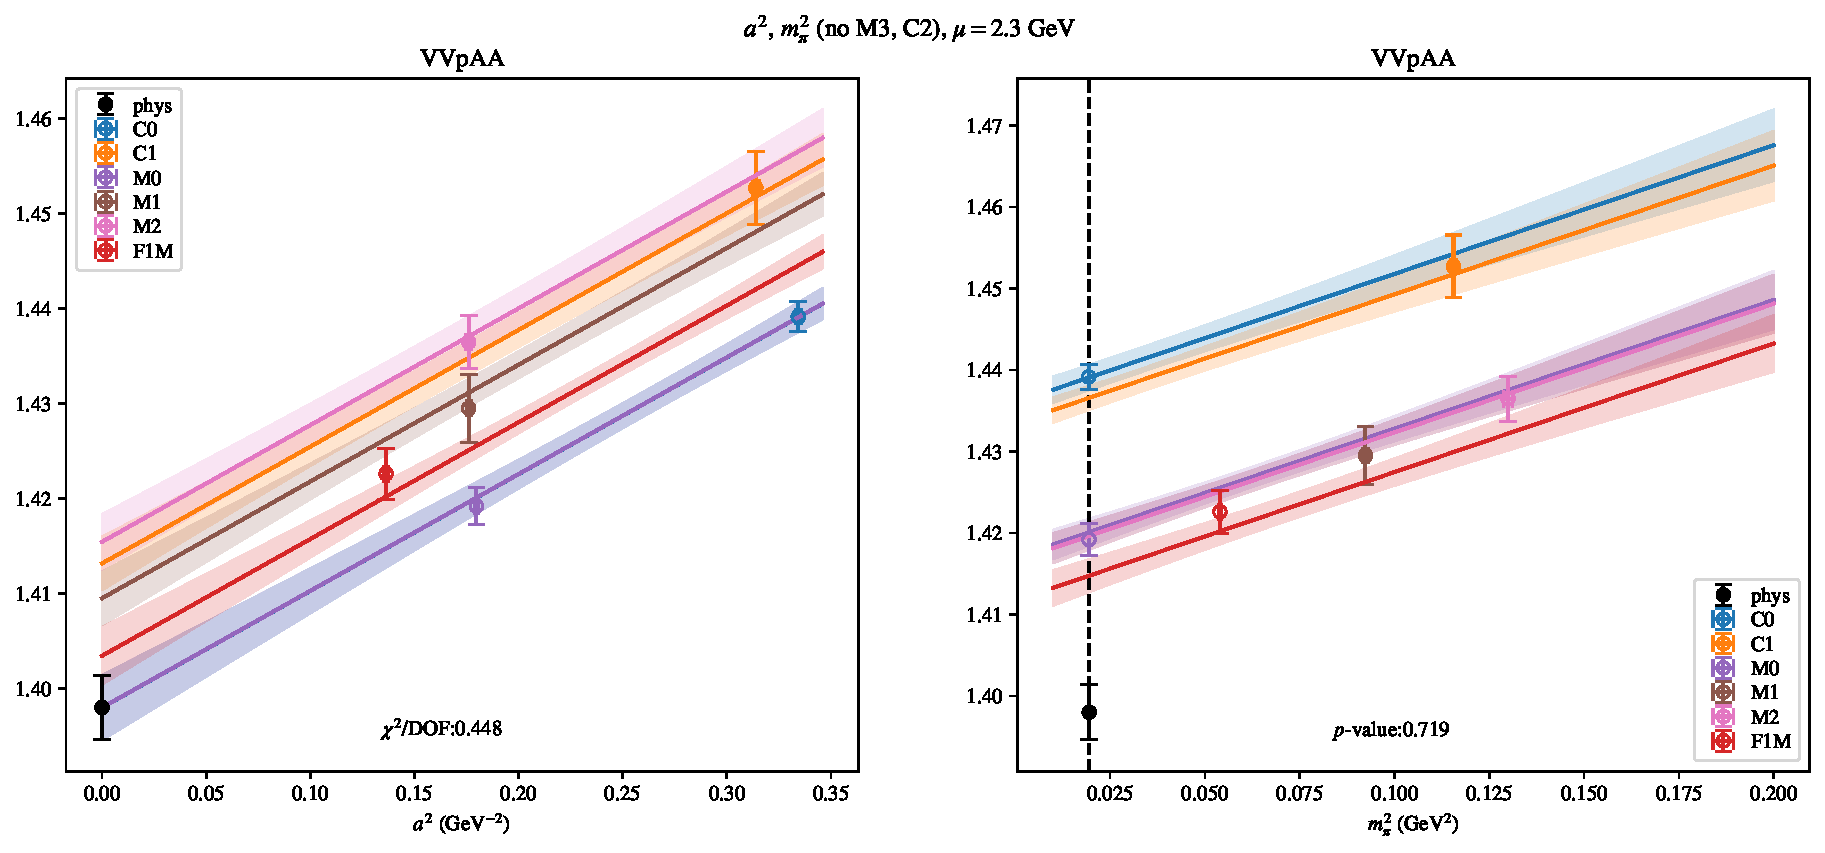
\includepdf[link, pages=-]{VVpAA/NPR/a2m2mcut_23.pdf}
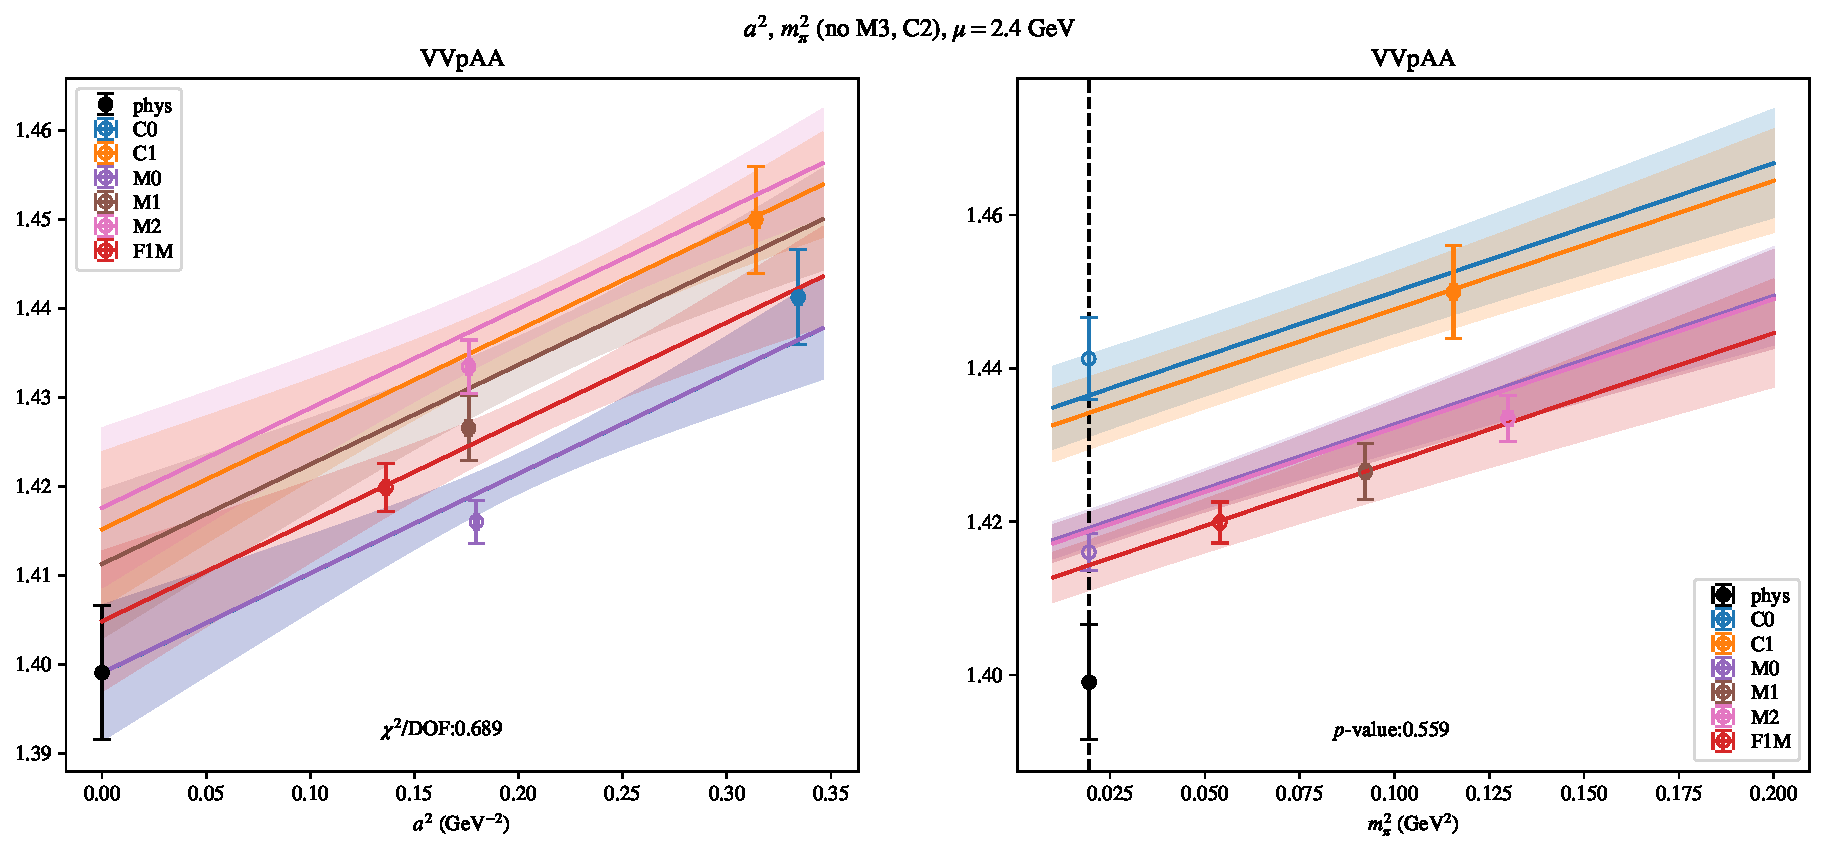
\includepdf[link, pages=-]{VVpAA/NPR/a2m2mcut_24.pdf}
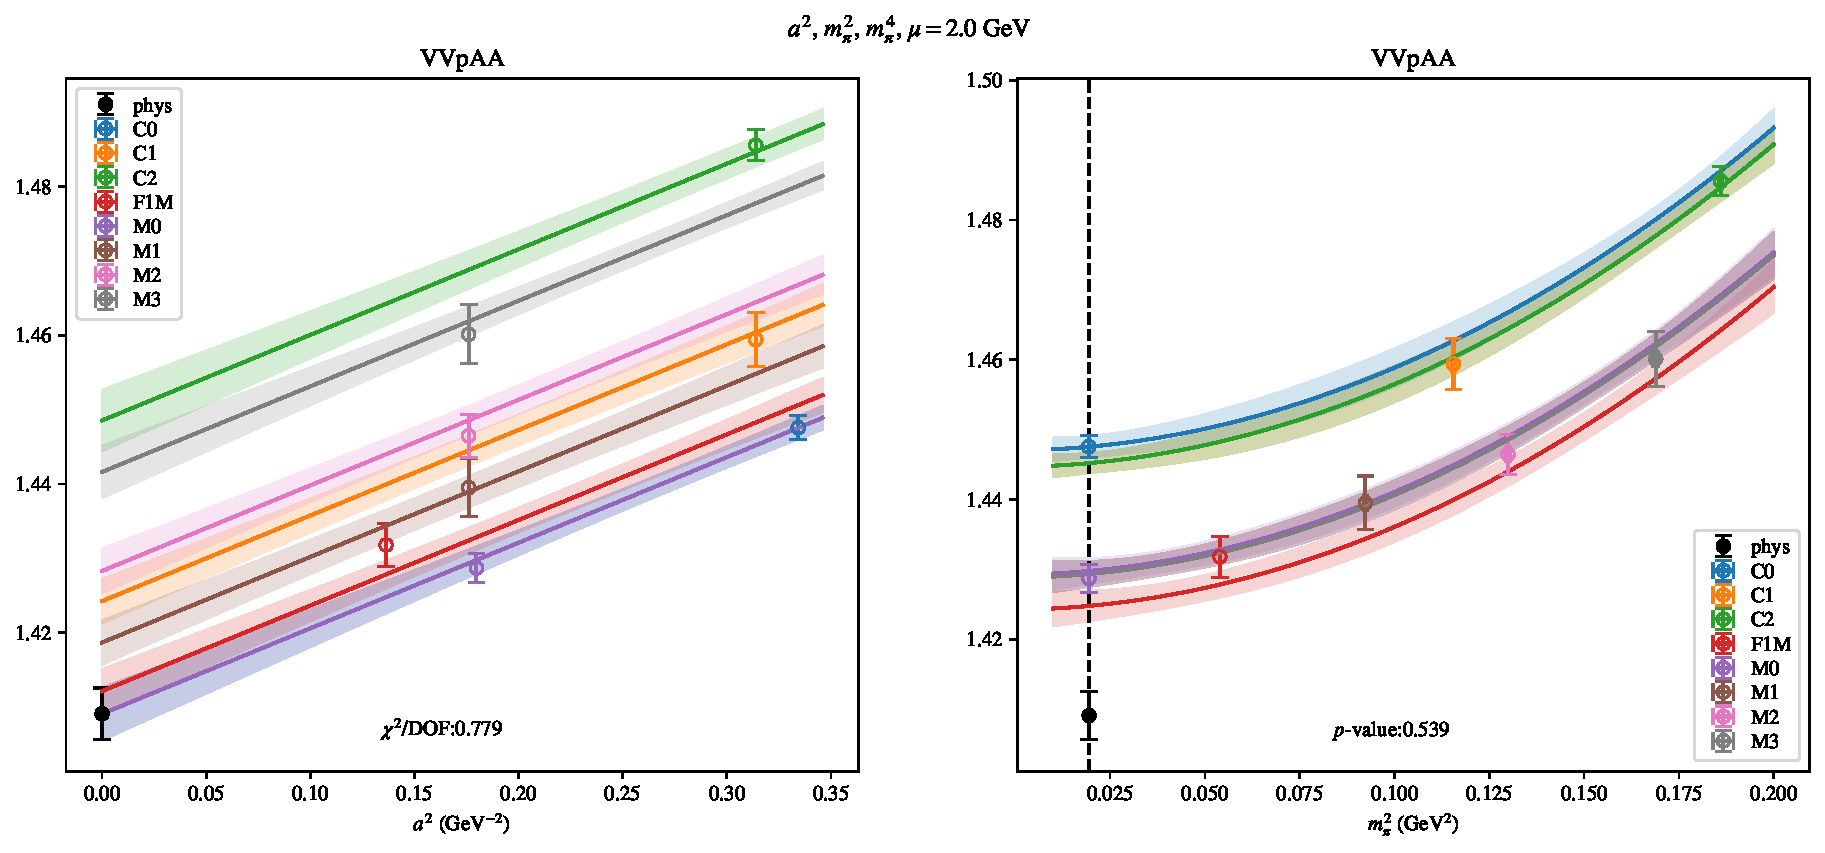
\includepdf[link, pages=-]{VVpAA/NPR/a2m2m4_20.pdf}
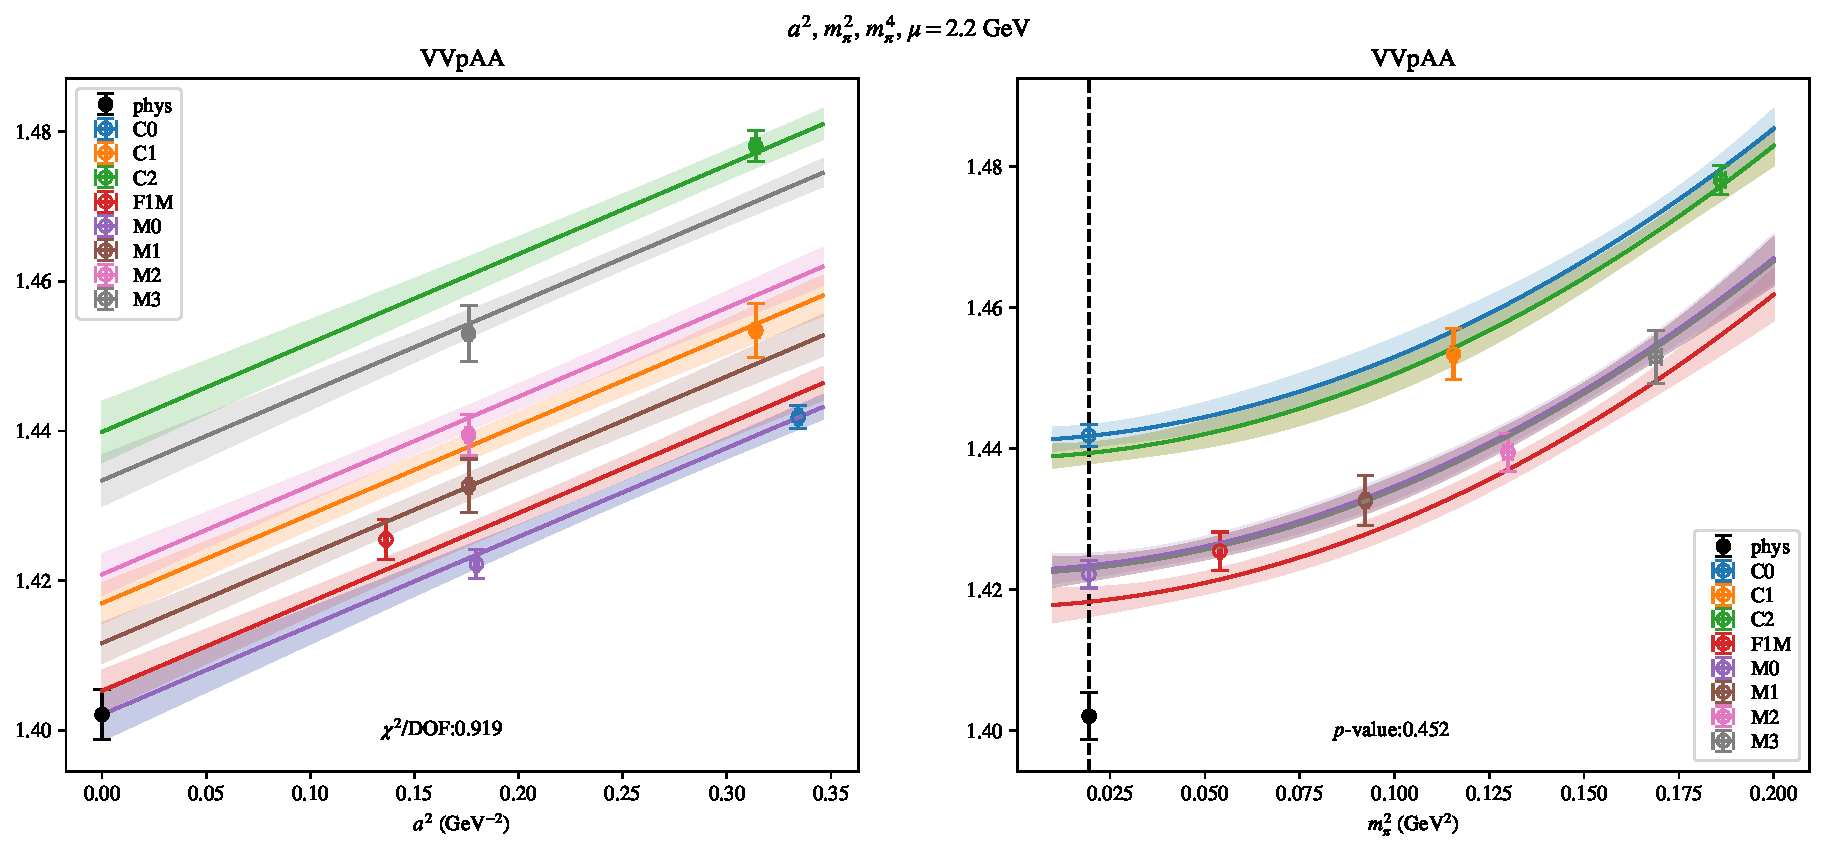
\includepdf[link, pages=-]{VVpAA/NPR/a2m2m4_22.pdf}
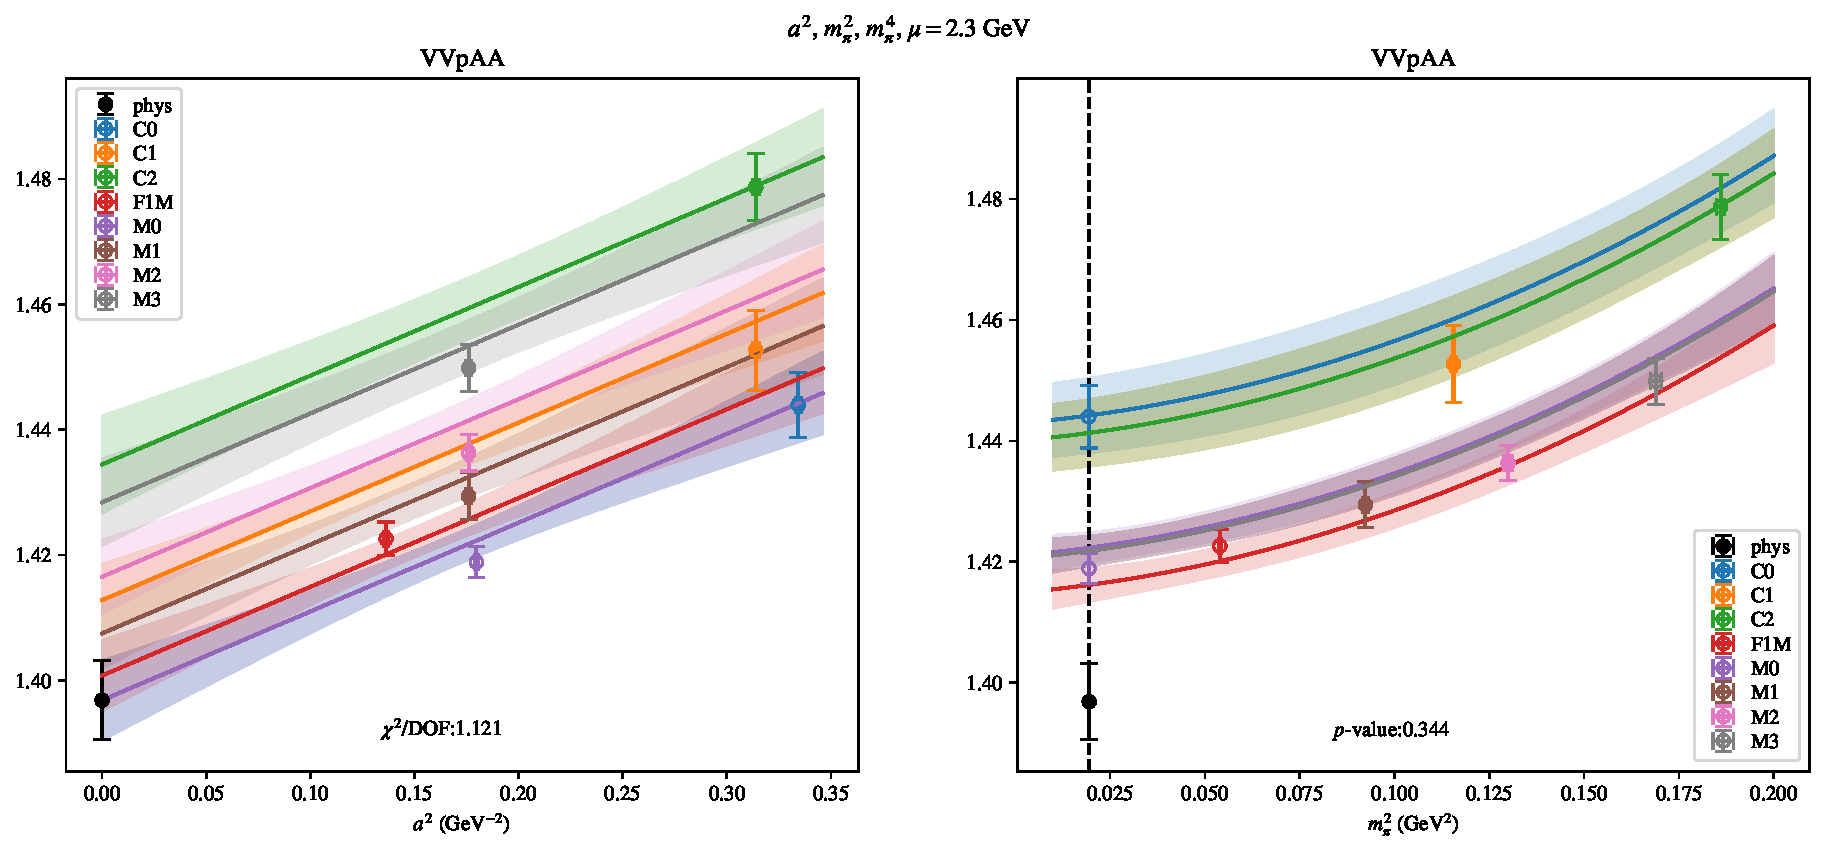
\includepdf[link, pages=-]{VVpAA/NPR/a2m2m4_23.pdf}
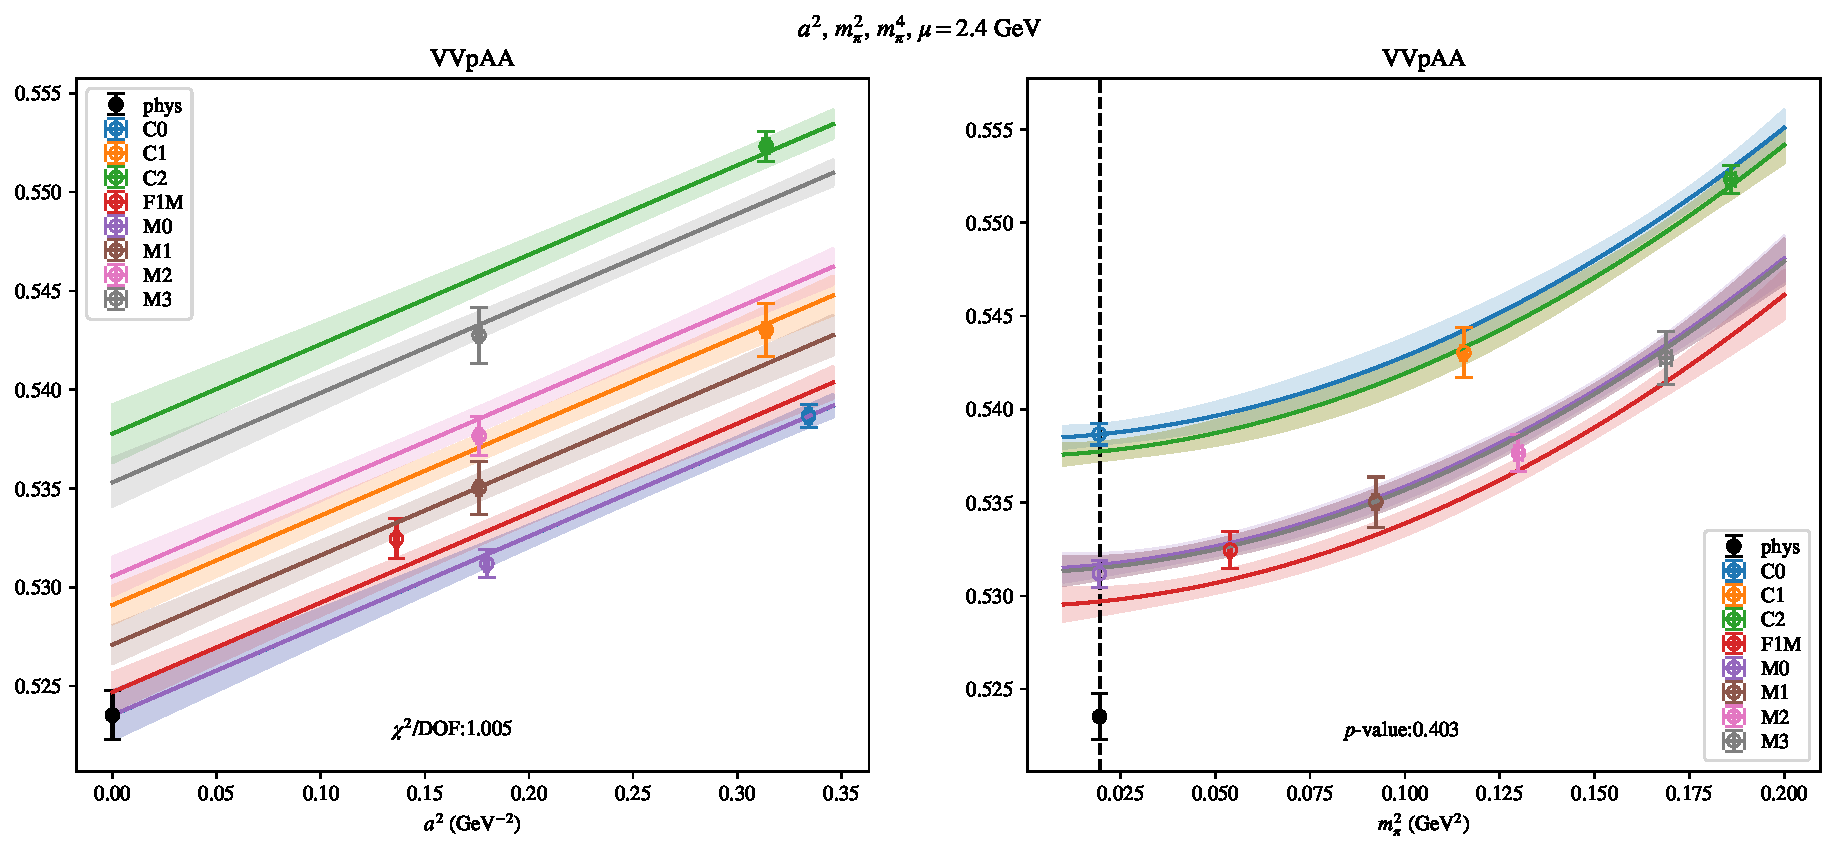
\includepdf[link, pages=-]{VVpAA/NPR/a2m2m4_24.pdf}
\clearpage
\section{$\mathcal{B}_2$}
\begin{table}[h!]
\begin{center}
\begin{tabular}{|c|c|c|c|c|c|}
\hline
$\mu$ (GeV) & $a^2$, $m_\pi^2$& $a^2$, $m_\pi^2$ (no C)& $a^2$, $a^4$, $m_\pi^2$& $a^2$, $m_\pi^2$ (no M3, C2)& $a^2$, $m_\pi^2$, $m_\pi^4$\\
\hline
2.0& \hyperlink{VVmAA/NPR/a2m2_20.pdf.1}{\textbf{-1.015(18)}: 3.286 (0.006)} & \hyperlink{VVmAA/NPR/a2m2noC_20.pdf.1}{\textbf{-0.98(12)}: 3.524 (0.029)} & \hyperlink{VVmAA/NPR/a2a4m2_20.pdf.1}{\textbf{-0.97(20)}: 2.999 (0.017)} & \hyperlink{VVmAA/NPR/a2m2mcut_20.pdf.1}{\textbf{-1.015(18)}: 4.285 (0.005)} & \hyperlink{VVmAA/NPR/a2m2m4_20.pdf.1}{\textbf{-1.016(18)}: 3.177 (0.013)}\\
2.2& \hyperlink{VVmAA/NPR/a2m2_22.pdf.1}{\textbf{-1.020(17)}: 4.299 (0.001)} & \hyperlink{VVmAA/NPR/a2m2noC_22.pdf.1}{\textbf{-0.986(92)}: 3.849 (0.021)} & \hyperlink{VVmAA/NPR/a2a4m2_22.pdf.1}{\textbf{-0.96(14)}: 2.251 (0.061)} & \hyperlink{VVmAA/NPR/a2m2mcut_22.pdf.1}{\textbf{-1.020(17)}: 5.505 (0.001)} & \hyperlink{VVmAA/NPR/a2m2m4_22.pdf.1}{\textbf{-1.021(17)}: 2.977 (0.018)}\\
2.3& \hyperlink{VVmAA/NPR/a2m2_23.pdf.1}{\textbf{-1.023(17)}: 4.56 (0.0)} & \hyperlink{VVmAA/NPR/a2m2noC_23.pdf.1}{\textbf{-0.988(90)}: 3.663 (0.026)} & \hyperlink{VVmAA/NPR/a2a4m2_23.pdf.1}{\textbf{-0.96(14)}: 2.157 (0.071)} & \hyperlink{VVmAA/NPR/a2m2mcut_23.pdf.1}{\textbf{-1.023(18)}: 6.01 (0.0)} & \hyperlink{VVmAA/NPR/a2m2m4_23.pdf.1}{\textbf{-1.025(17)}: 3.255 (0.011)}\\
2.4& \hyperlink{VVmAA/NPR/a2m2_24.pdf.1}{\textbf{-1.026(17)}: 5.124 (0.0)} & \hyperlink{VVmAA/NPR/a2m2noC_24.pdf.1}{\textbf{-0.990(88)}: 4.195 (0.015)} & \hyperlink{VVmAA/NPR/a2a4m2_24.pdf.1}{\textbf{-0.97(14)}: 2.682 (0.03)} & \hyperlink{VVmAA/NPR/a2m2mcut_24.pdf.1}{\textbf{-1.026(17)}: 6.609 (0.0)} & \hyperlink{VVmAA/NPR/a2m2m4_24.pdf.1}{\textbf{-1.028(17)}: 3.749 (0.005)}\\
\hline
\end{tabular}
\caption{Physical point value from chiral and continuum extrapolation at renormalisation scale $\mu$. Entries are \textbf{value(error)}: $\chi^2/\text{DOF}$ ($p$-value).}
\end{center}
\end{table}
\begin{table}[h!]
\begin{center}
\begin{tabular}{|c c|c|c|c|c|c|}
\hline
$\mu$ (GeV) &  & $a^2$, $m_\pi^2$& $a^2$, $m_\pi^2$ (no C)& $a^2$, $a^4$, $m_\pi^2$& $a^2$, $m_\pi^2$ (no M3, C2)& $a^2$, $m_\pi^2$, $m_\pi^4$\\
\hline
\multirow{2}{0.5in}{2.0} & $\alpha$ & -0.186(63)& 0.007& 0.16(19)& -0.184(64)& -0.189(64)\\
 & $\beta$ & 0.00192(21)& 0.00232(28)& 0.00194(21)& 0.00178(29)& 0.00013(84)\\
\hline
\multirow{2}{0.5in}{2.2} & $\alpha$ & -0.224(63)& -0.03(52)& 0.23(13)& -0.224(60)& -0.229(62)\\
 & $\beta$ & 0.00167(18)& 0.00177(23)& 0.00164(17)& 0.00130(25)& -0.0006(73)\\
\hline
\multirow{2}{0.5in}{2.3} & $\alpha$ & -0.245(62)& -0.05(51)& 0.23(13)& -0.246(62)& -0.251(60)\\
 & $\beta$ & 0.00155(18)& 0.00164(23)& 0.00152(19)& 0.00120(25)& -0.0008(71)\\
\hline
\multirow{2}{0.5in}{2.4} & $\alpha$ & -0.266(60)& -0.07(50)& 0.20(13)& -0.267(60)& -0.272(62)\\
 & $\beta$ & 0.00149(16)& 0.00160(21)& 0.00143(16)& 0.00113(23)& -0.0008(68)\\
\hline
\end{tabular}
\caption{Fit values of coefficients in $Q = Q_{phys} + \mathbf{\alpha} a^2 + \mathbf{\beta}\left(\frac{m_\pi^2}{f_\pi^2}-\frac{m_{\pi,PDG}^2}{f_\pi^2}\right) + \ldots$.}
\end{center}
\end{table}
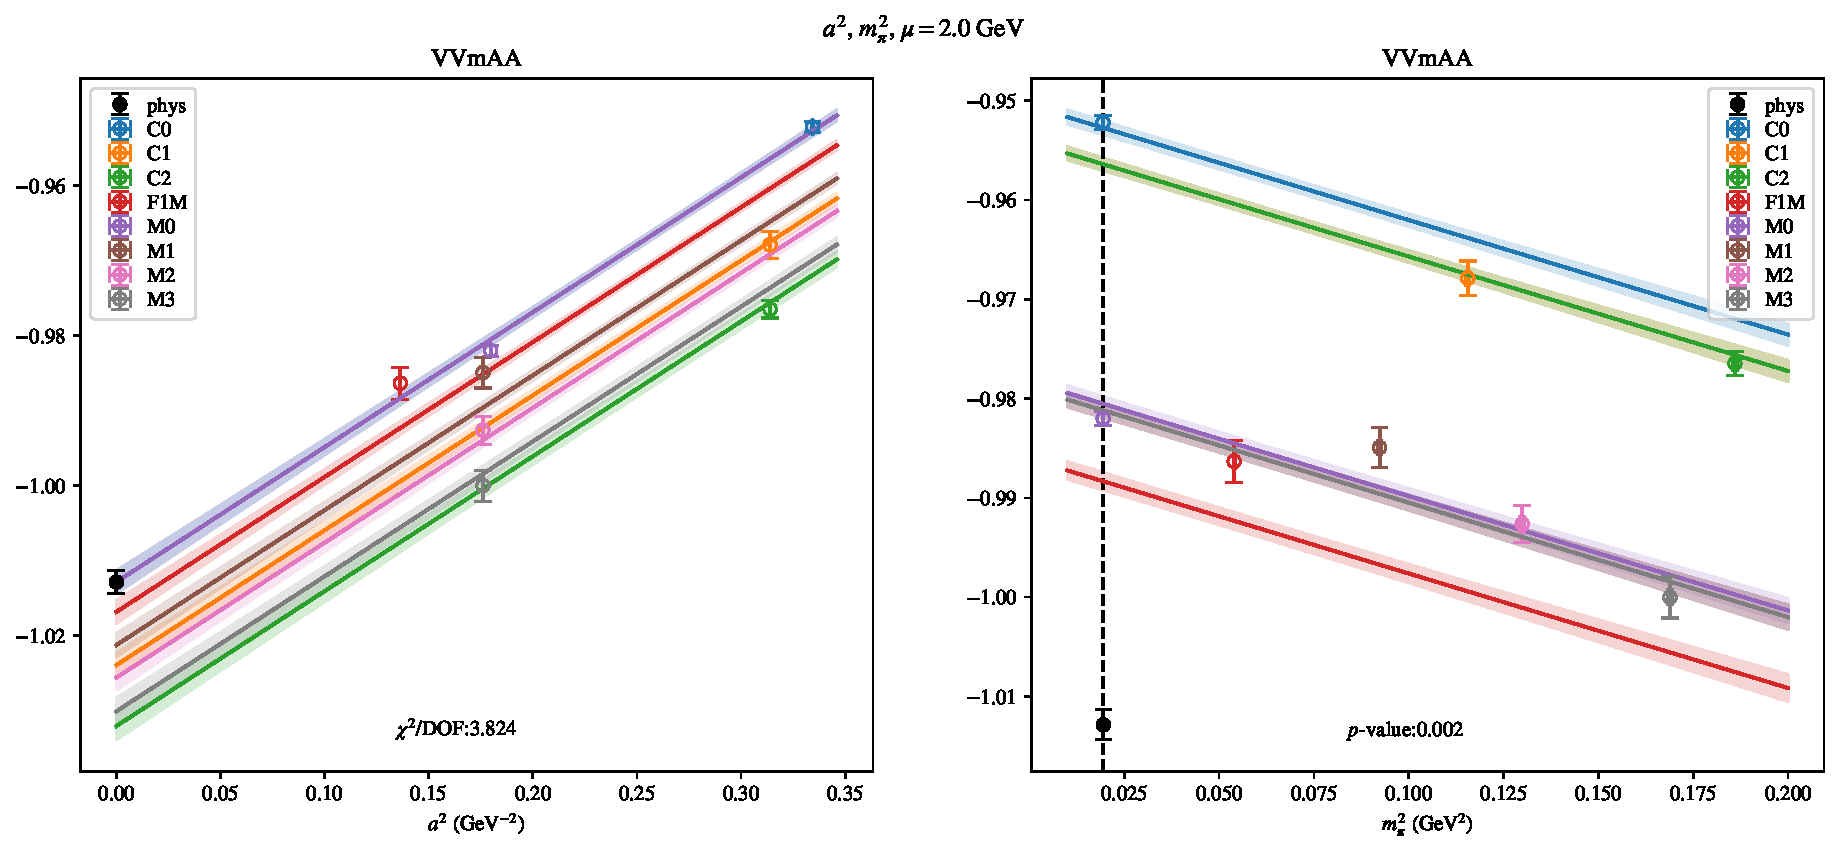
\includepdf[link, pages=-]{VVmAA/NPR/a2m2_20.pdf}
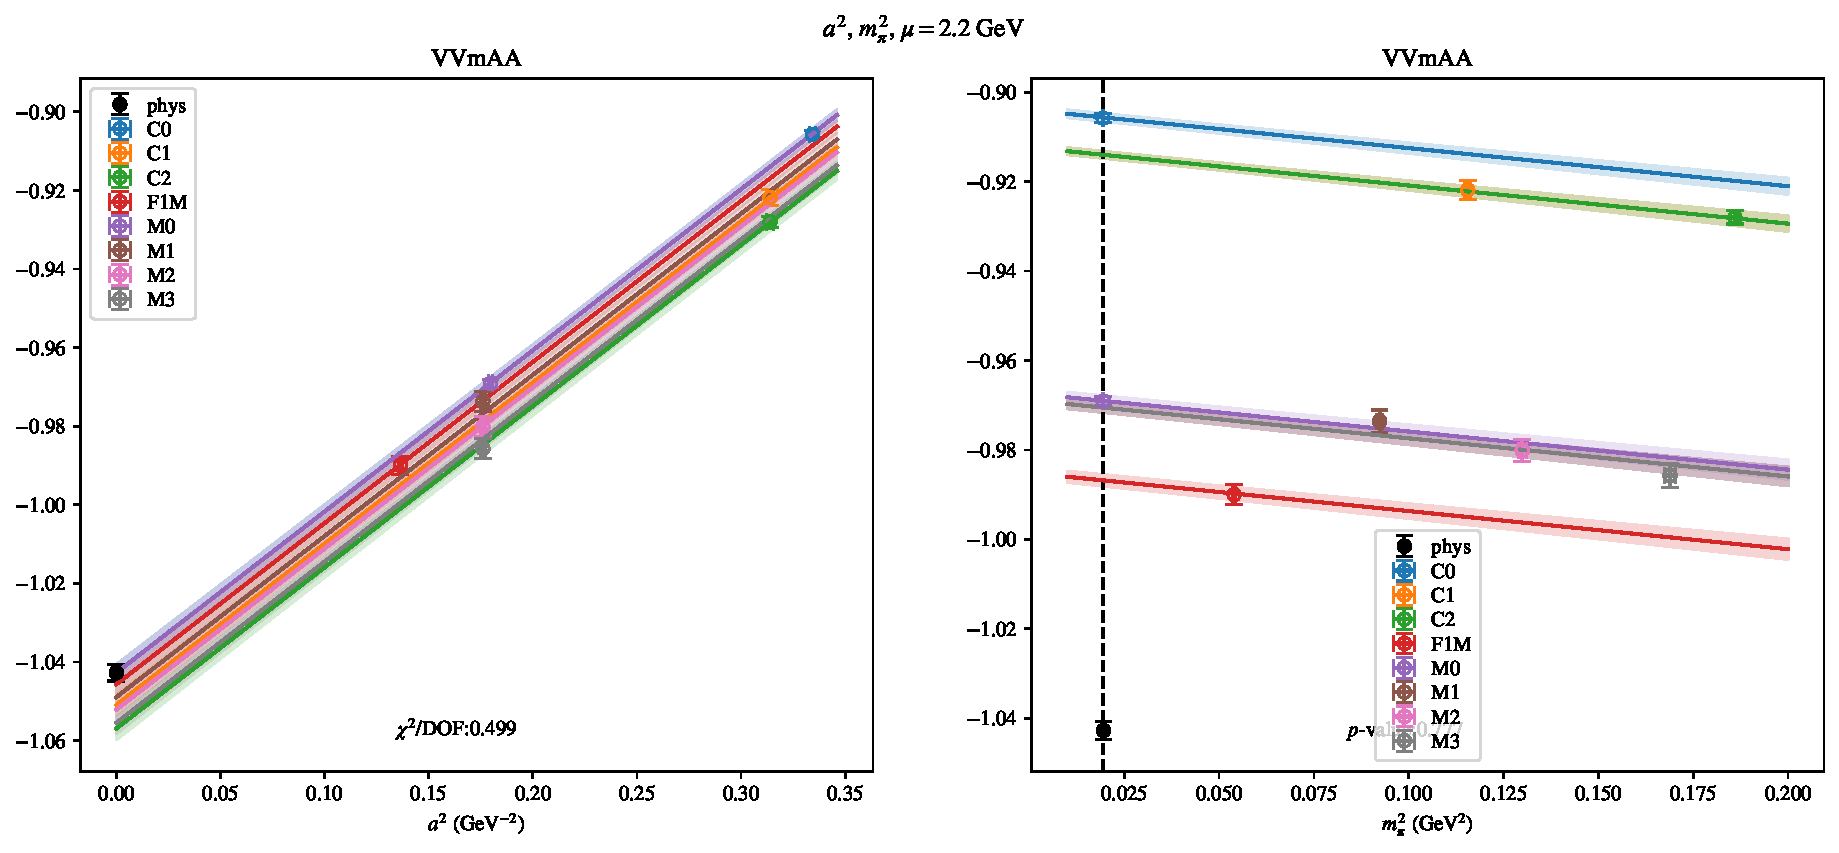
\includepdf[link, pages=-]{VVmAA/NPR/a2m2_22.pdf}
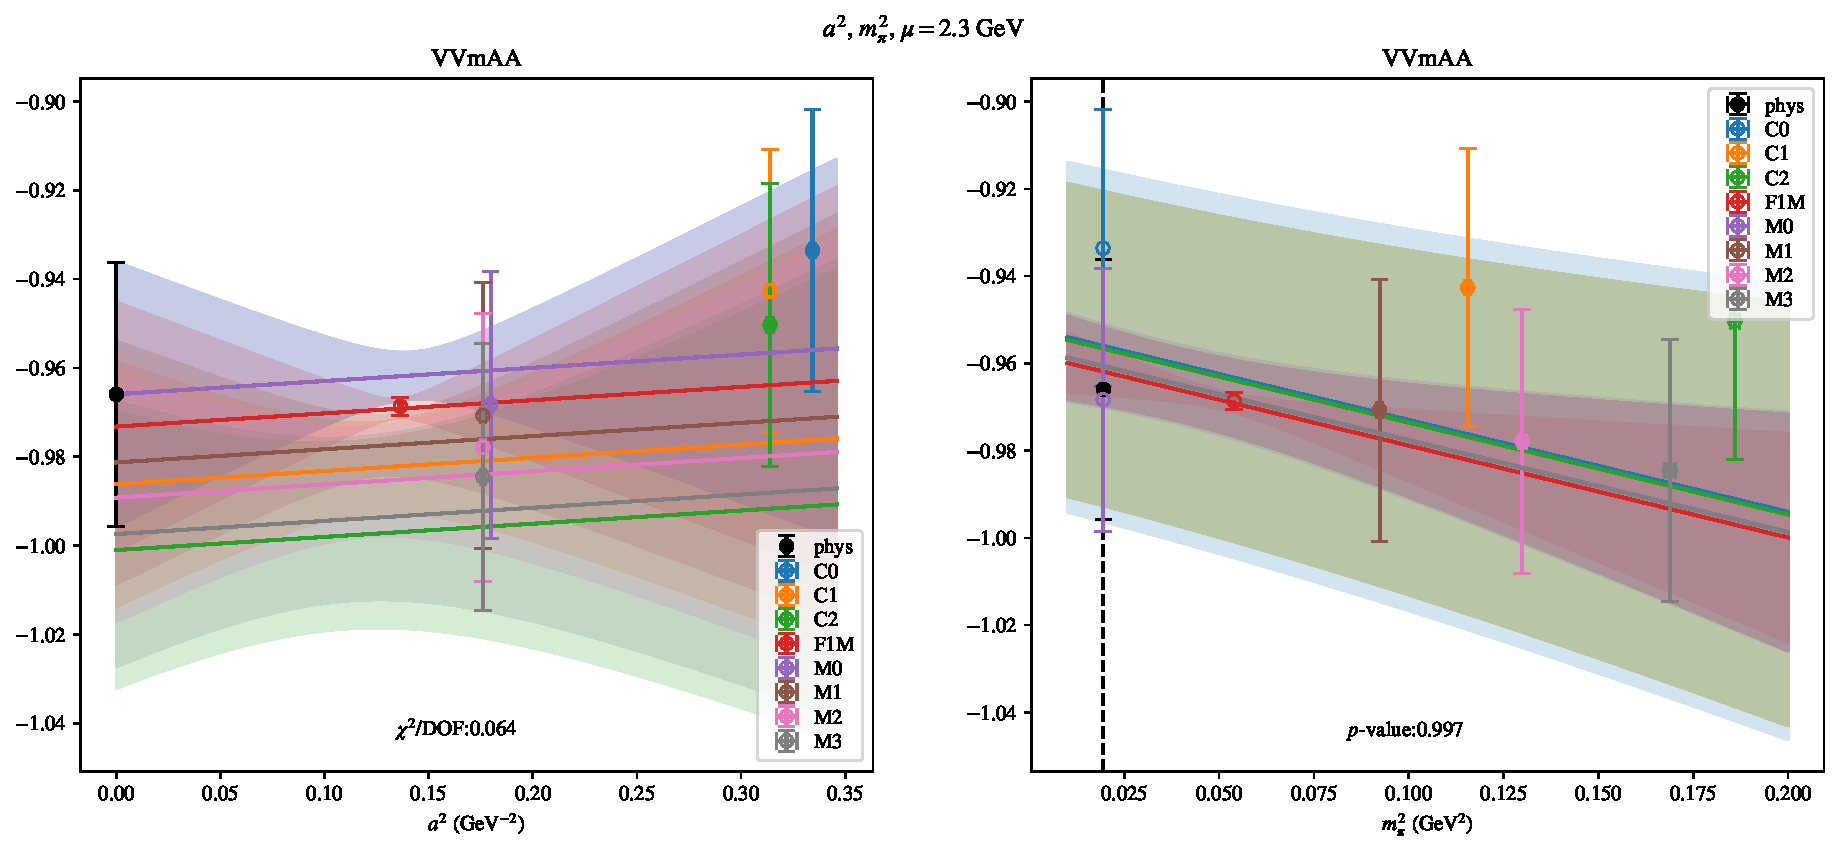
\includepdf[link, pages=-]{VVmAA/NPR/a2m2_23.pdf}
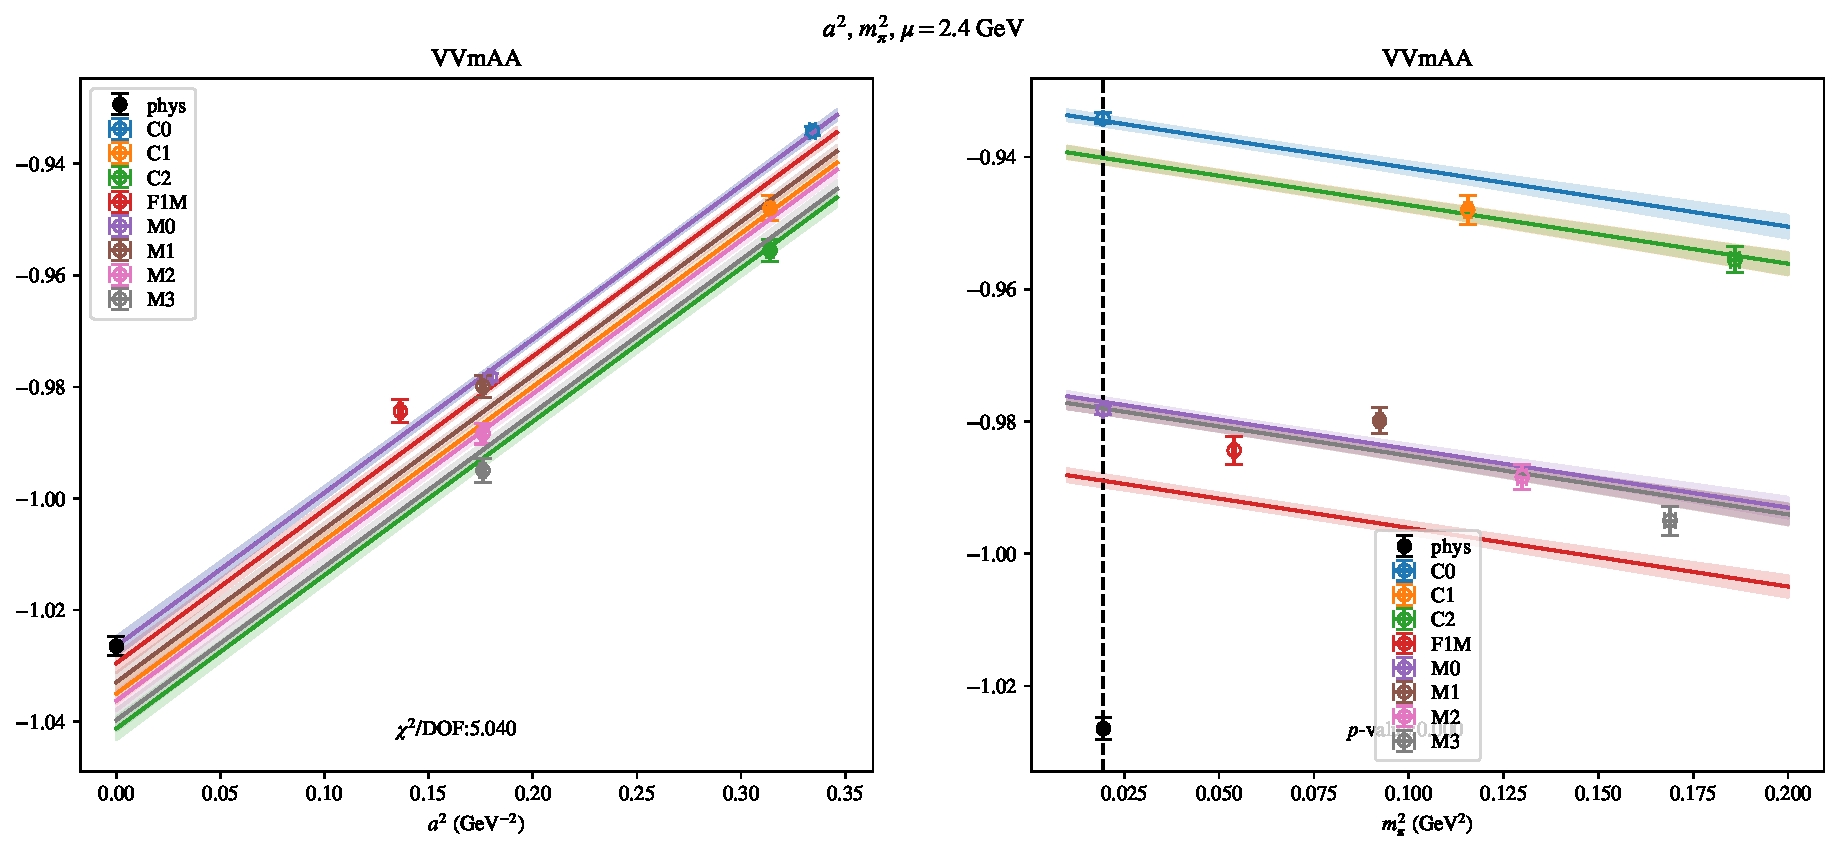
\includepdf[link, pages=-]{VVmAA/NPR/a2m2_24.pdf}
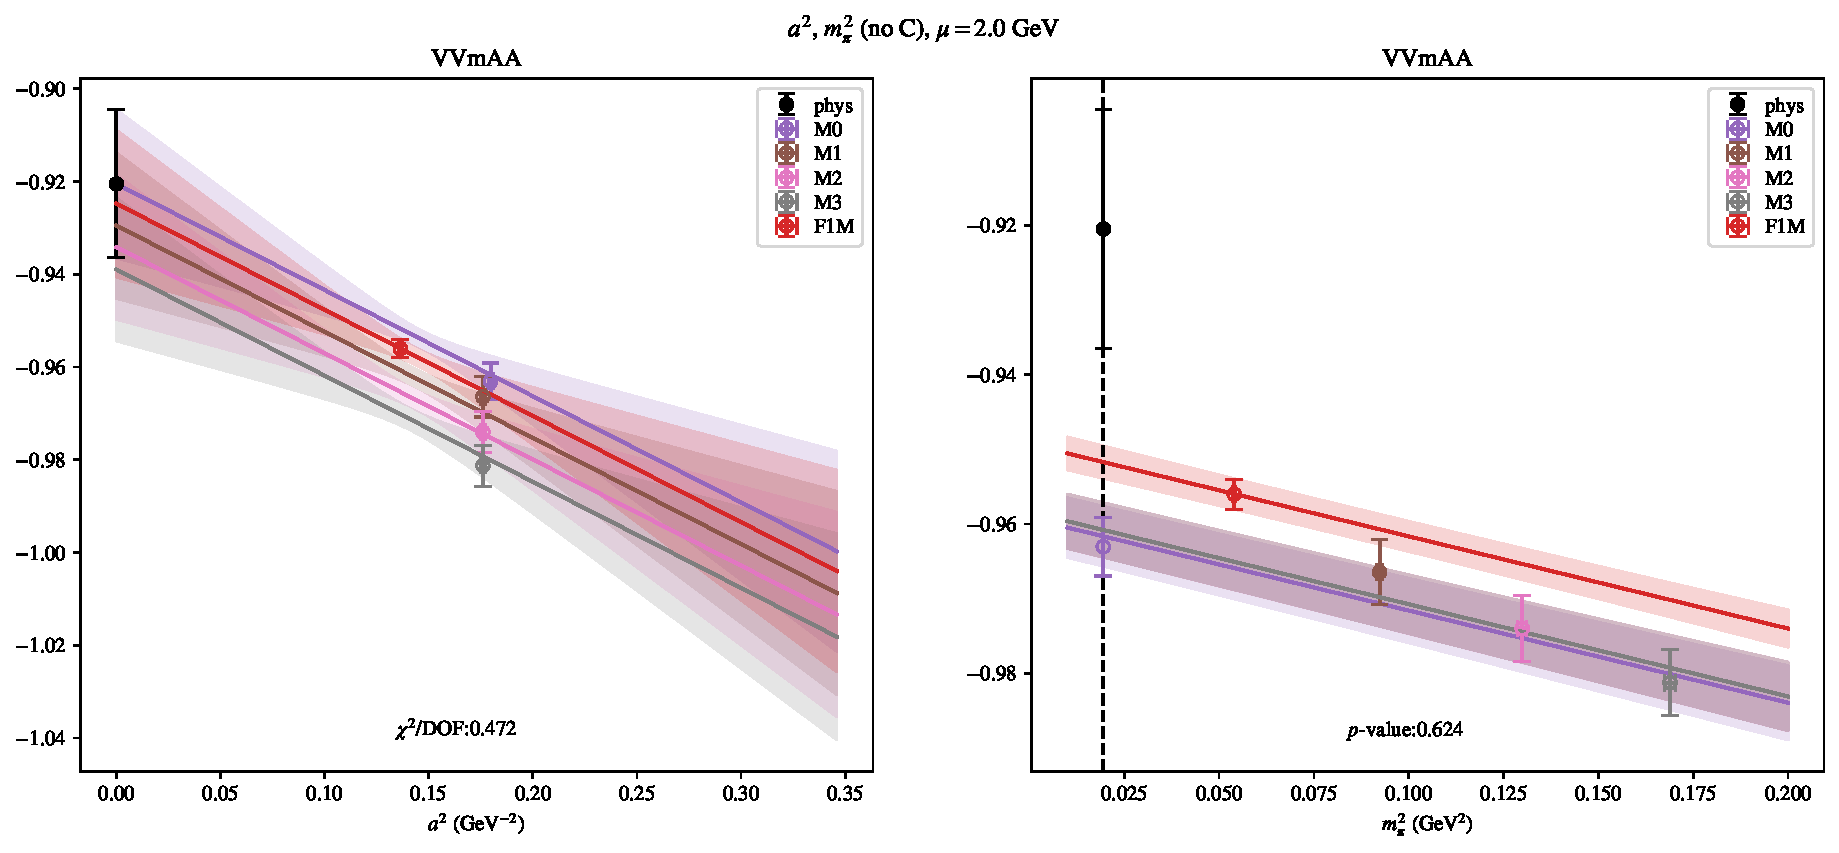
\includepdf[link, pages=-]{VVmAA/NPR/a2m2noC_20.pdf}
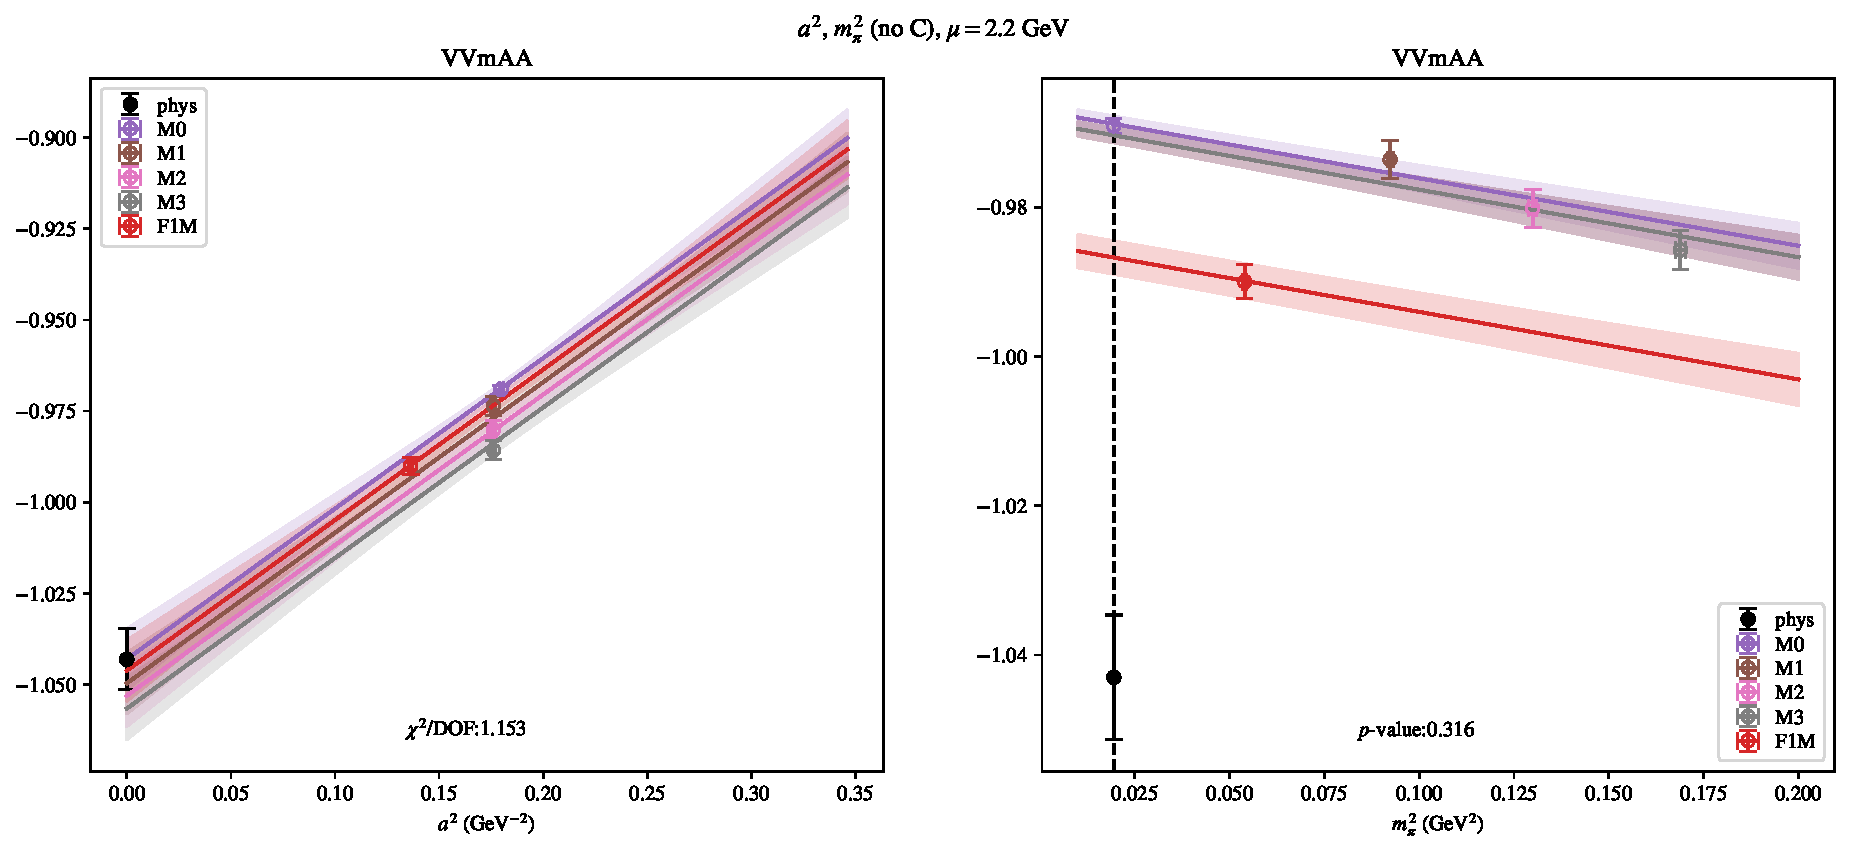
\includepdf[link, pages=-]{VVmAA/NPR/a2m2noC_22.pdf}
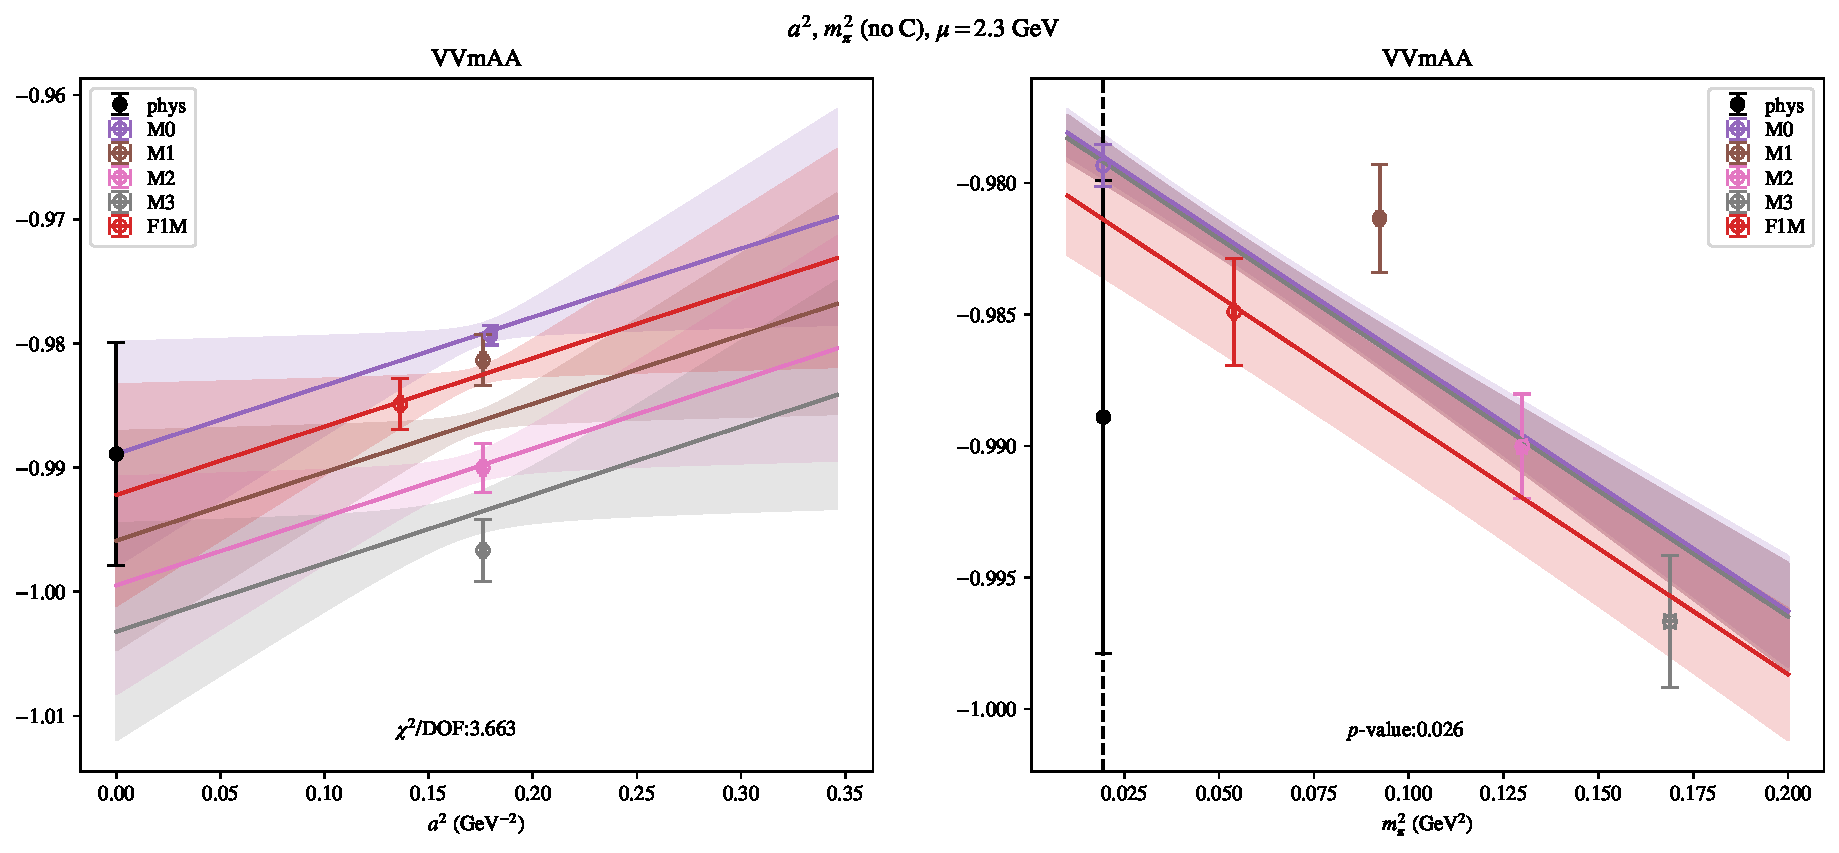
\includepdf[link, pages=-]{VVmAA/NPR/a2m2noC_23.pdf}
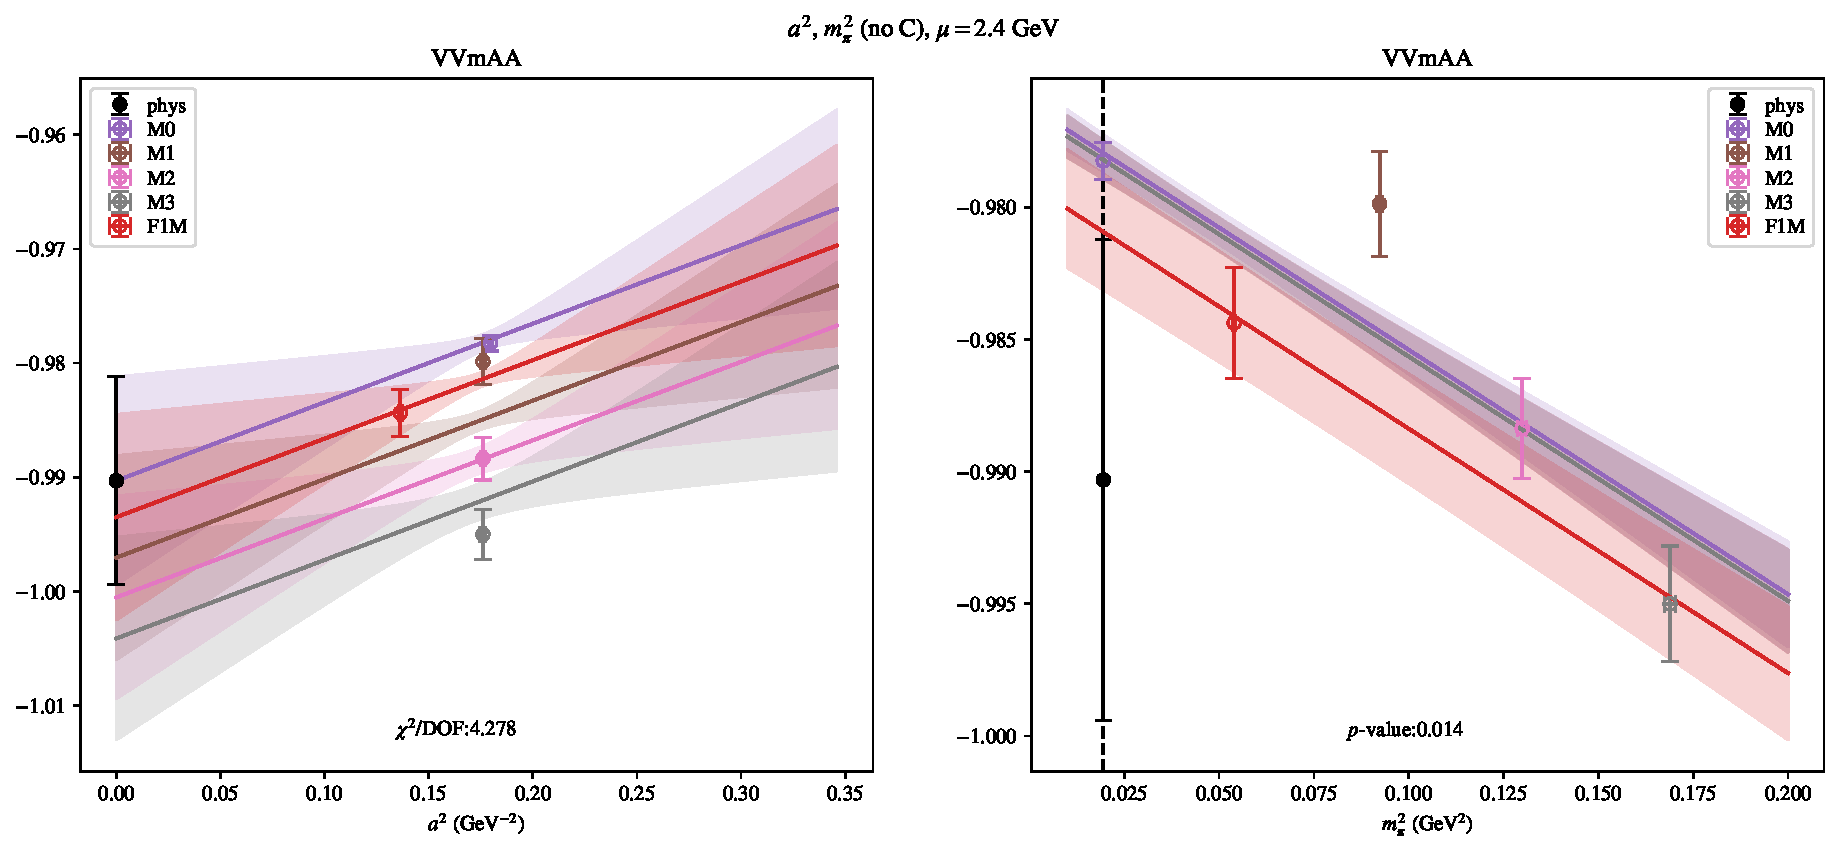
\includepdf[link, pages=-]{VVmAA/NPR/a2m2noC_24.pdf}
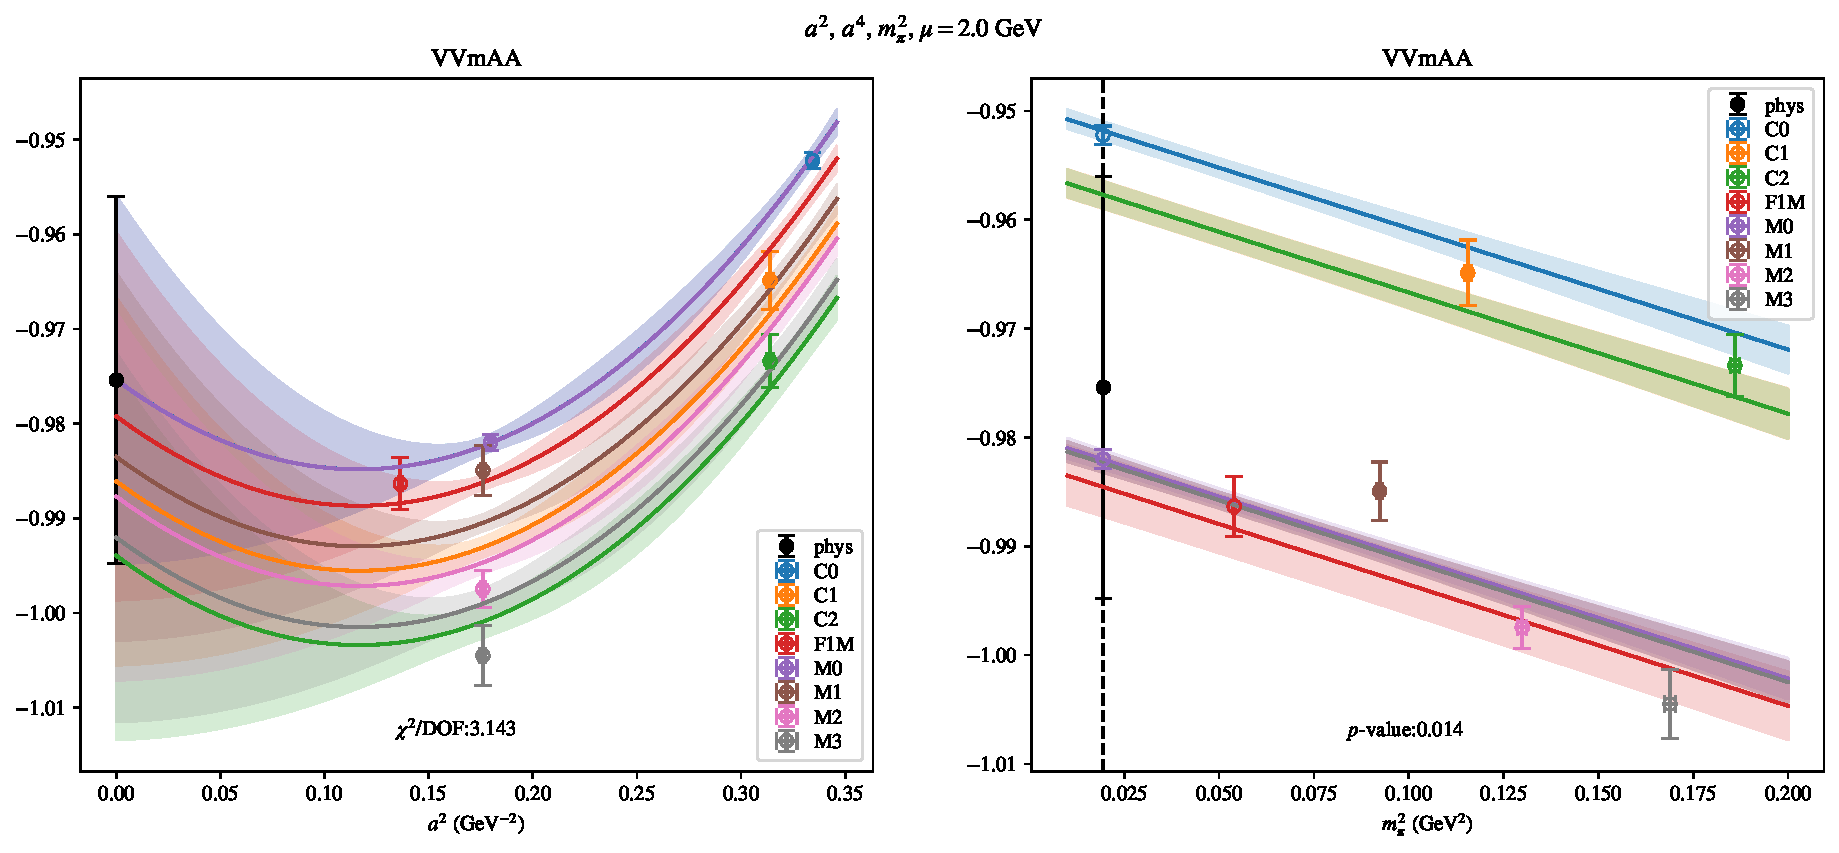
\includepdf[link, pages=-]{VVmAA/NPR/a2a4m2_20.pdf}
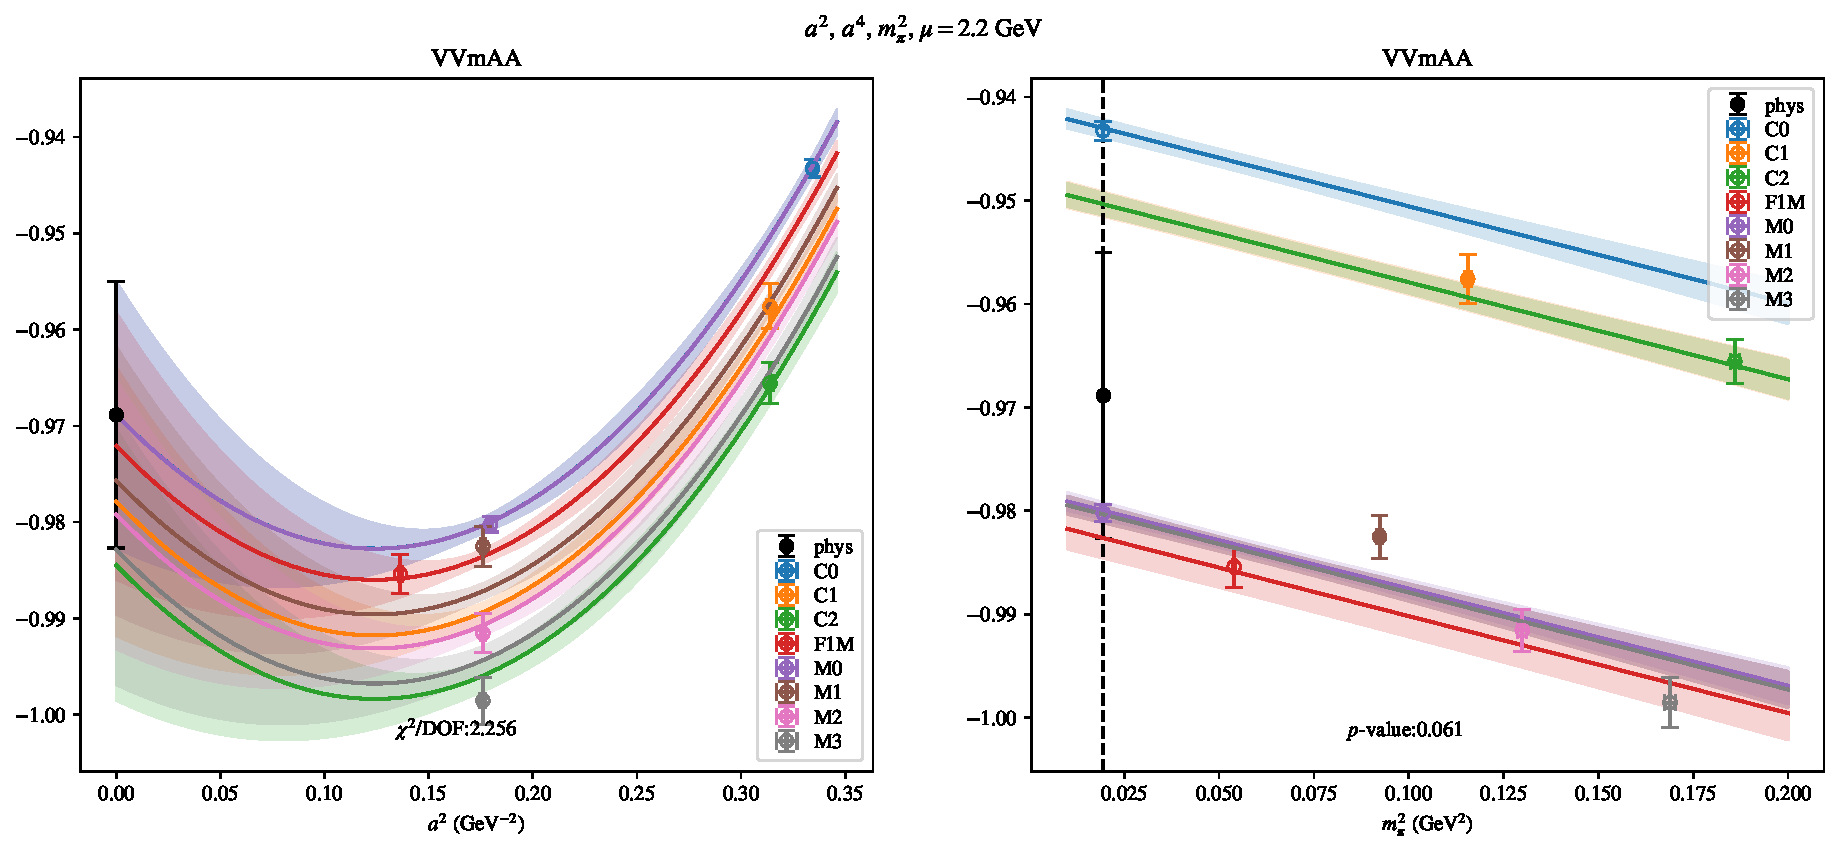
\includepdf[link, pages=-]{VVmAA/NPR/a2a4m2_22.pdf}
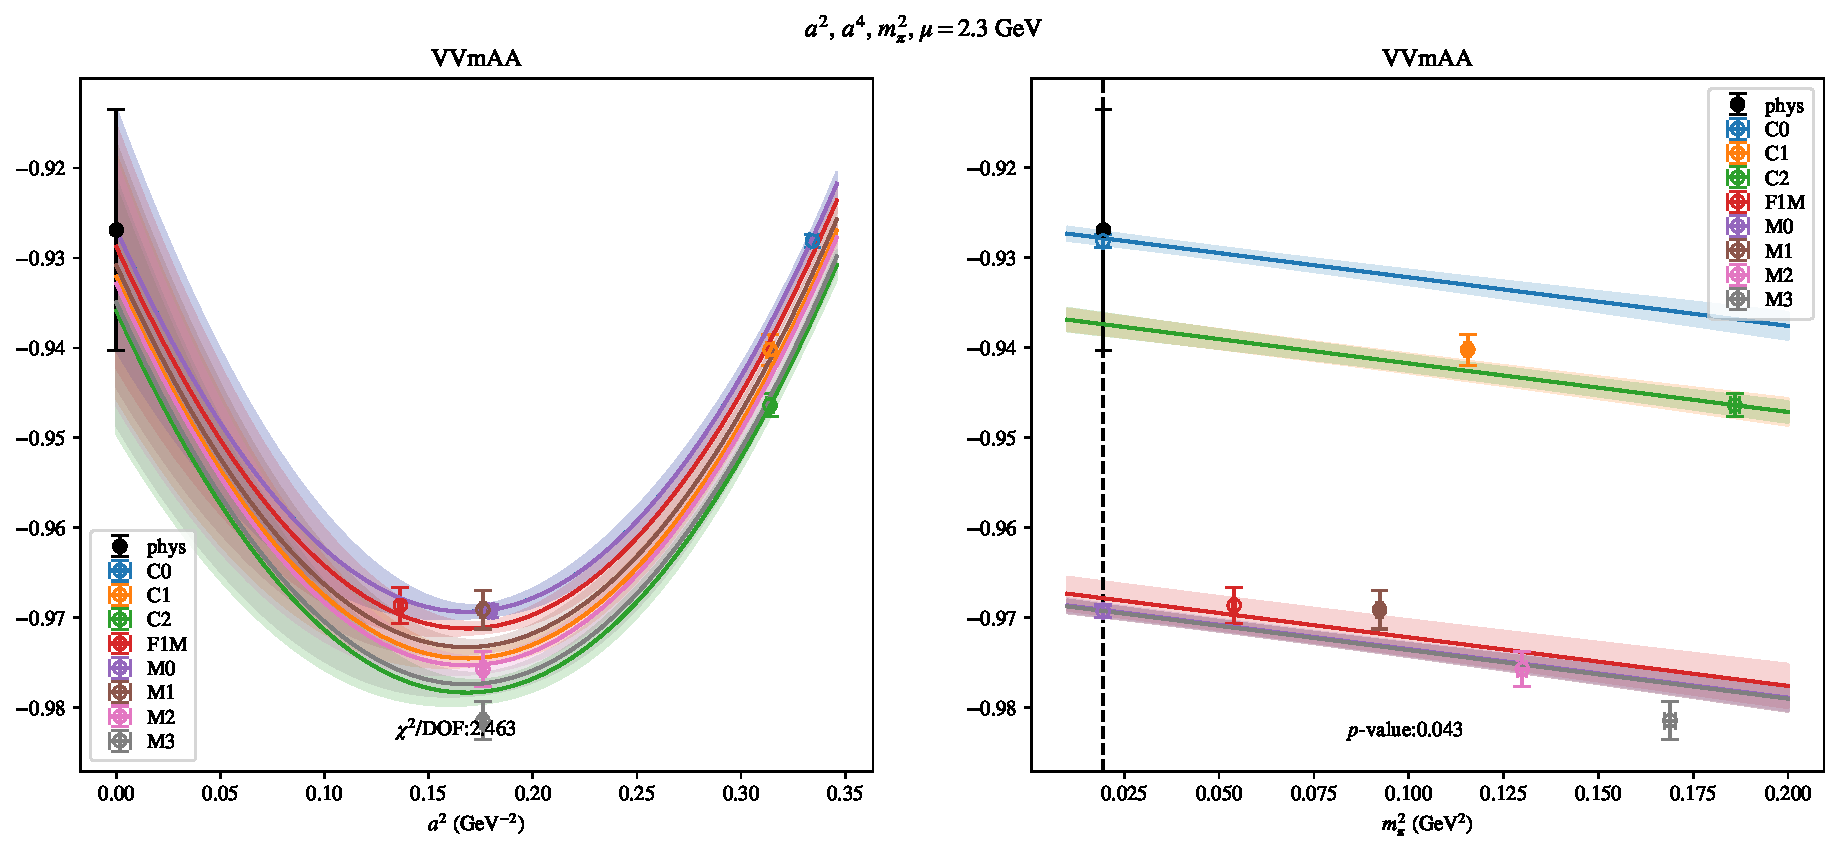
\includepdf[link, pages=-]{VVmAA/NPR/a2a4m2_23.pdf}
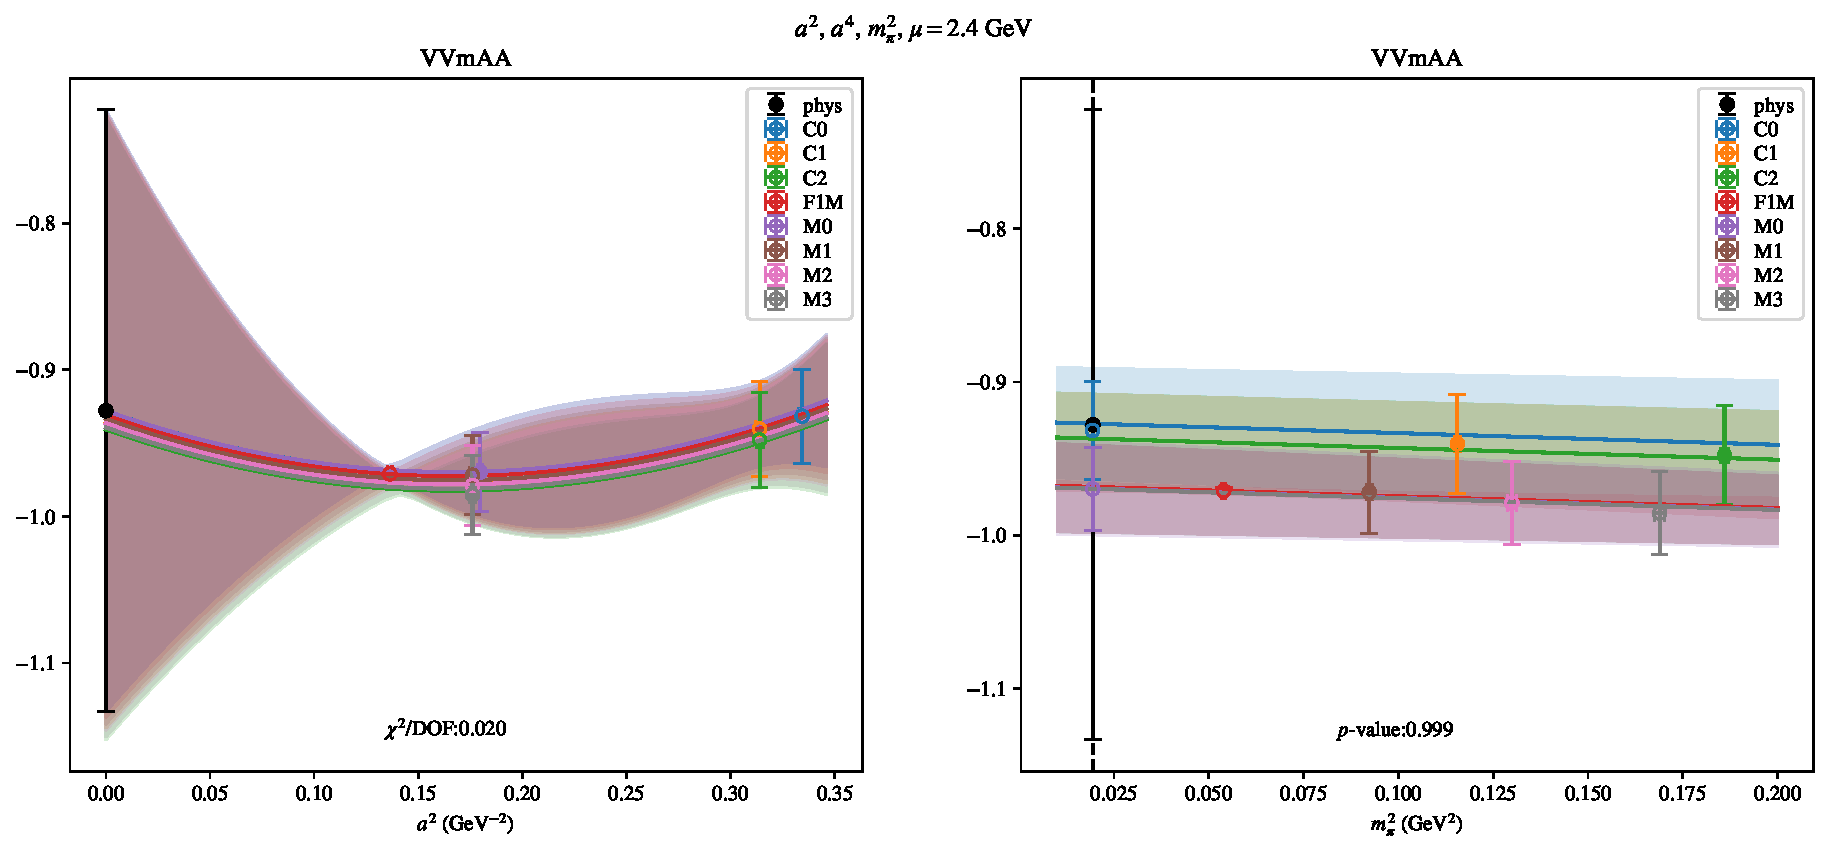
\includepdf[link, pages=-]{VVmAA/NPR/a2a4m2_24.pdf}
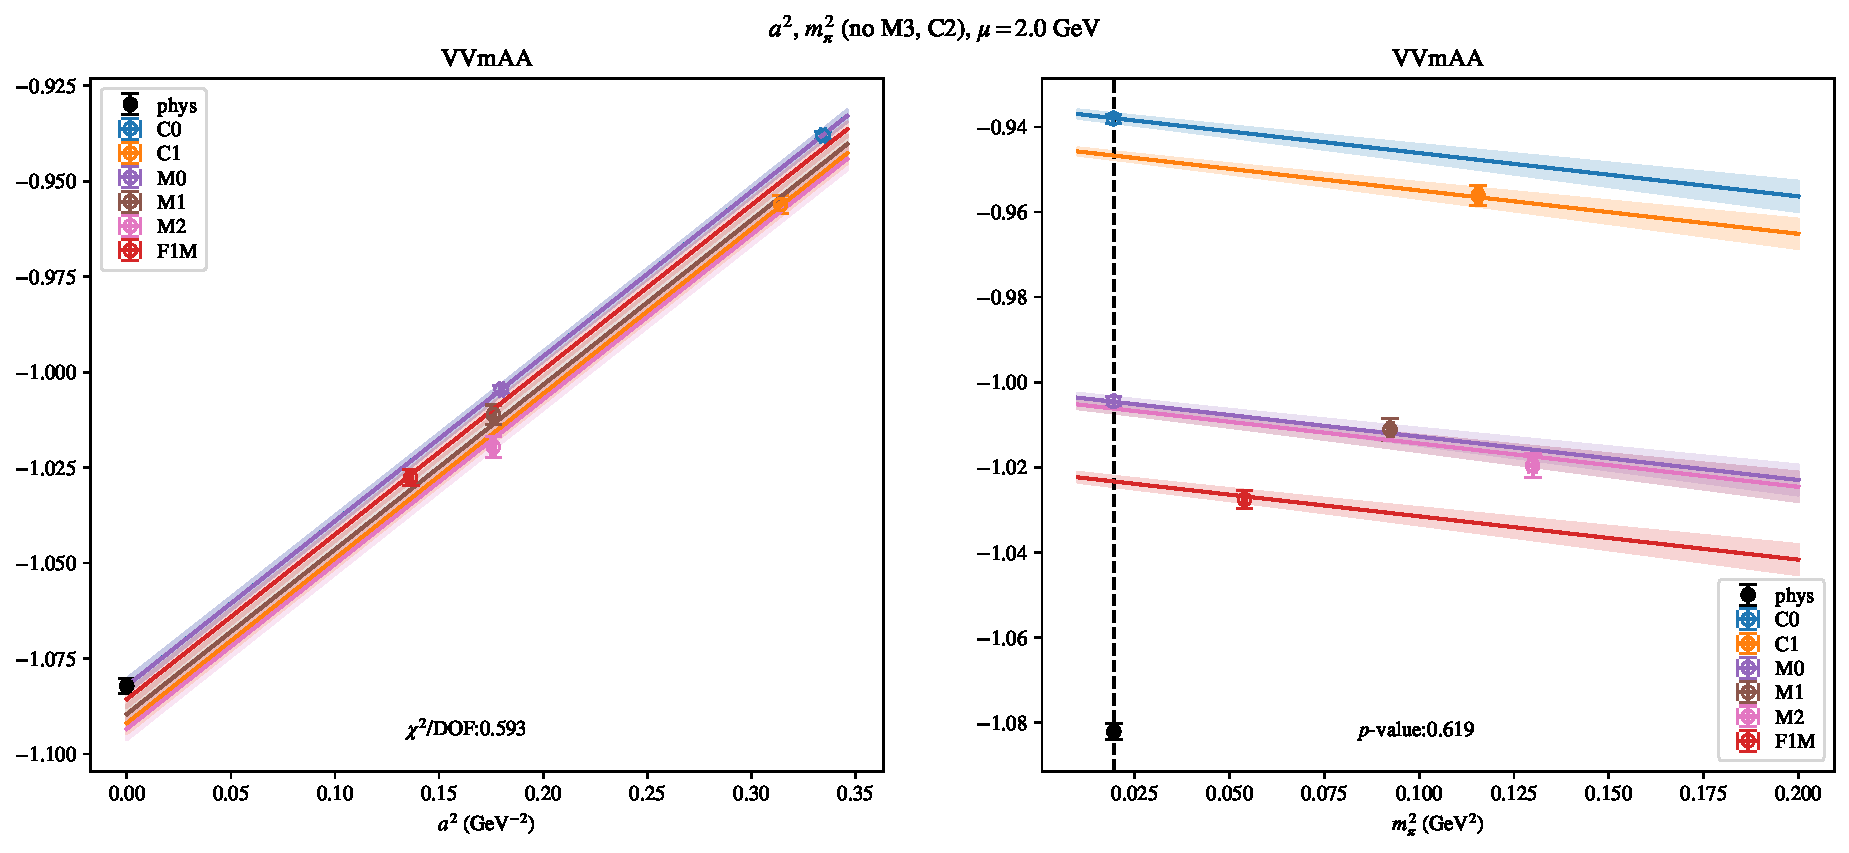
\includepdf[link, pages=-]{VVmAA/NPR/a2m2mcut_20.pdf}
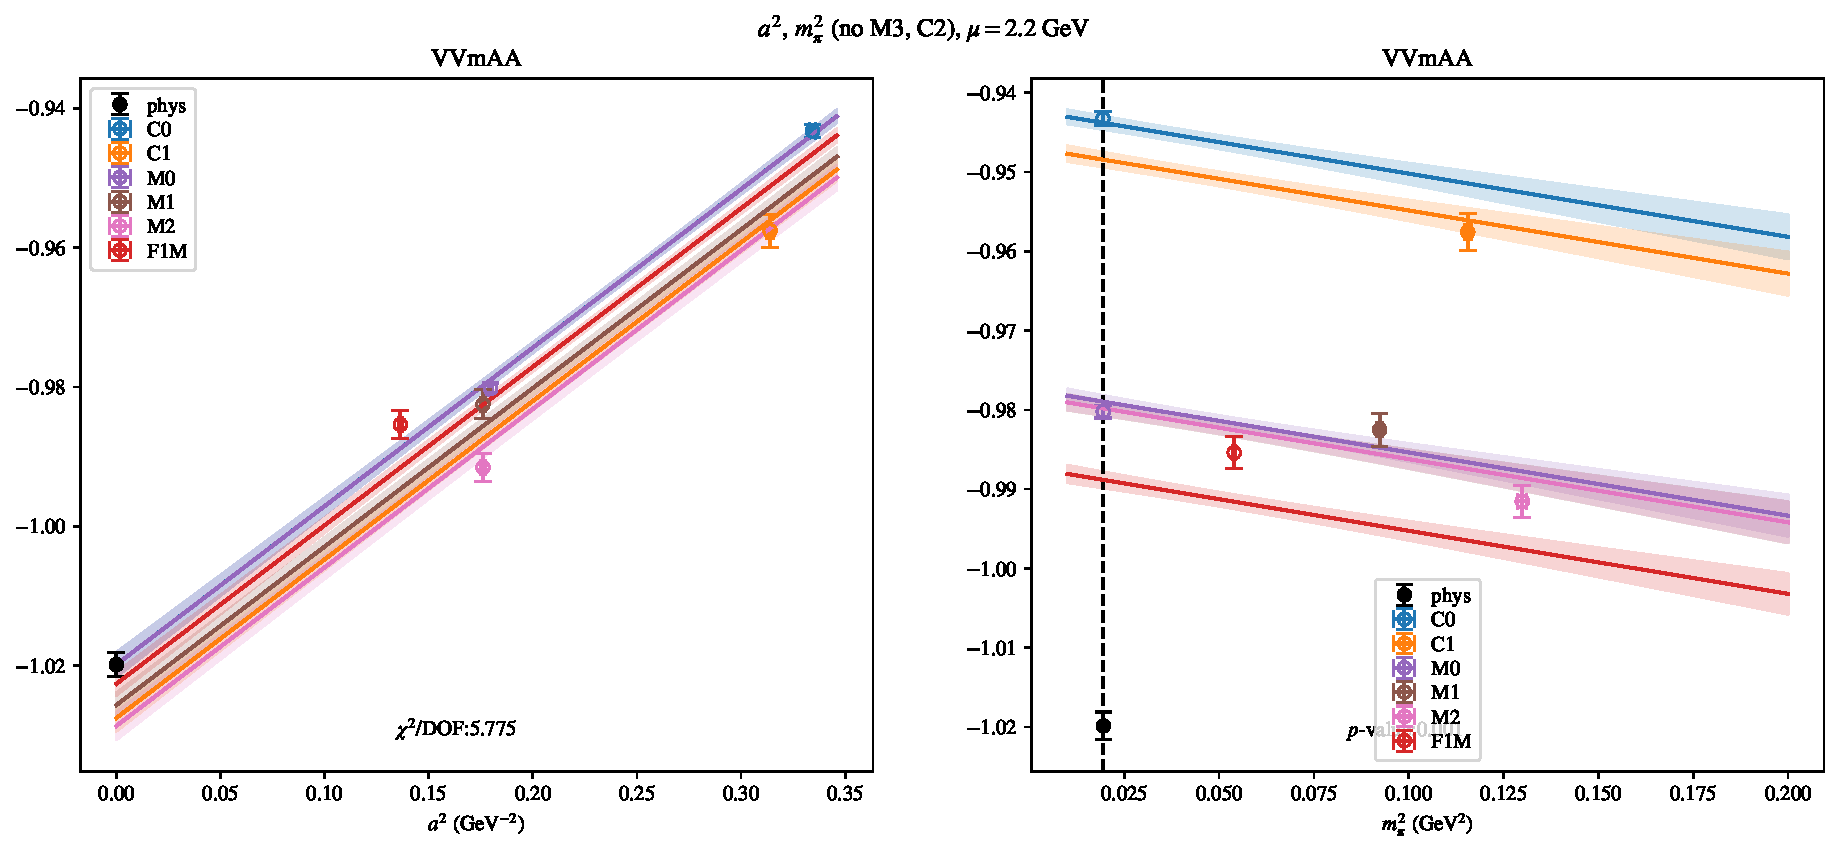
\includepdf[link, pages=-]{VVmAA/NPR/a2m2mcut_22.pdf}
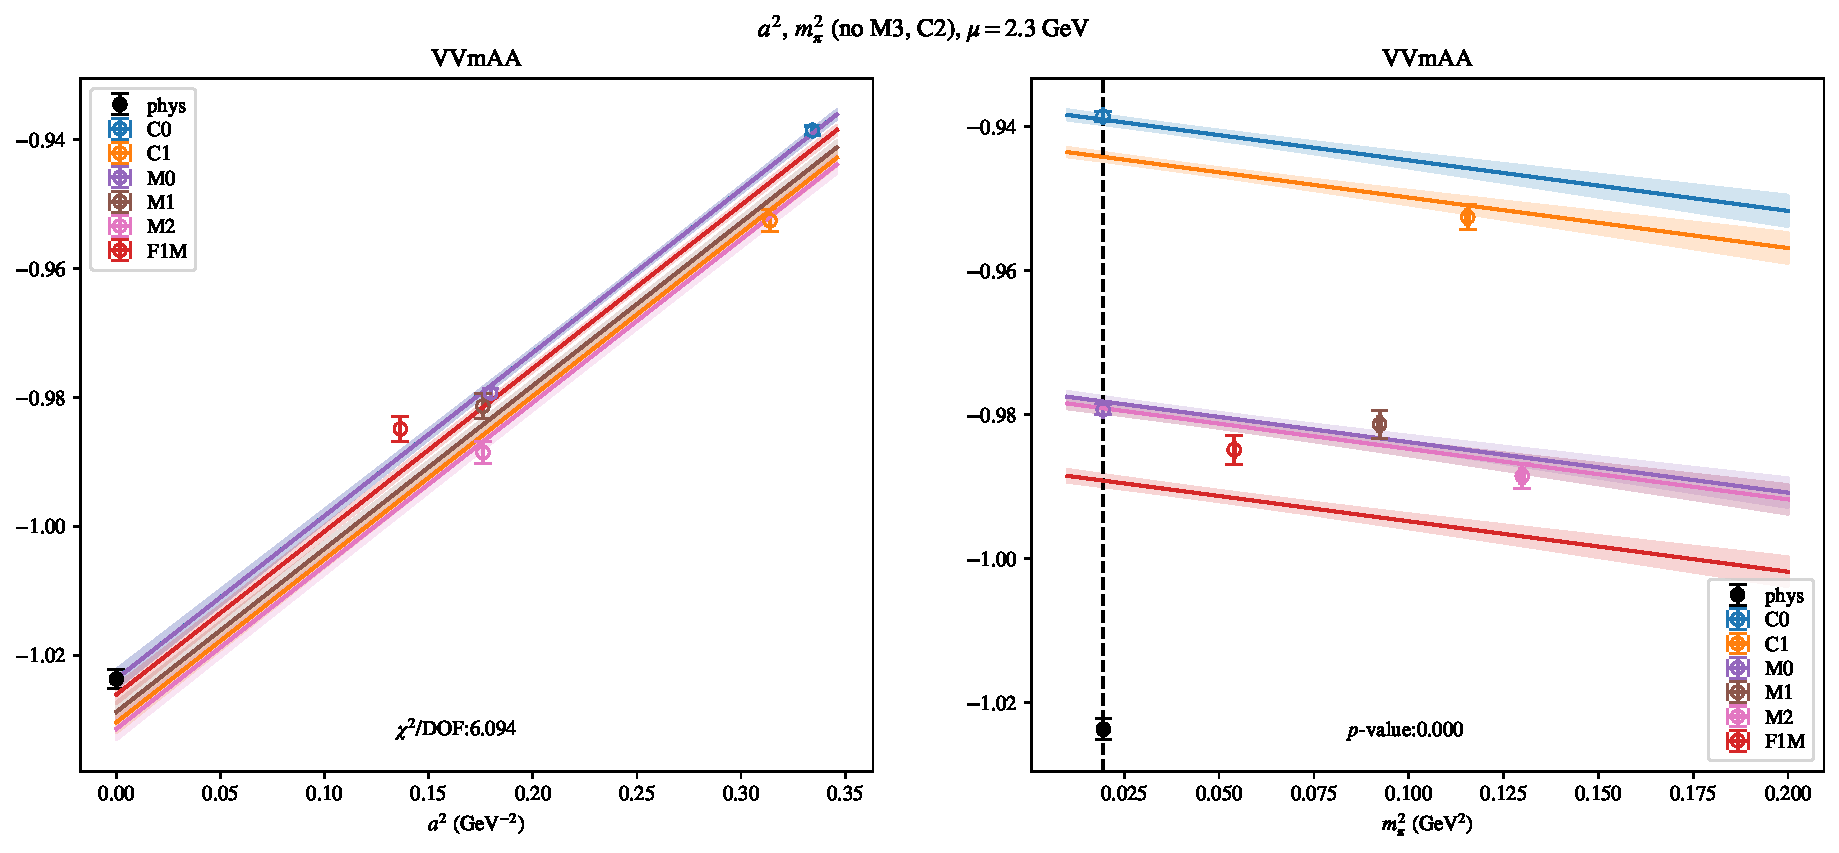
\includepdf[link, pages=-]{VVmAA/NPR/a2m2mcut_23.pdf}
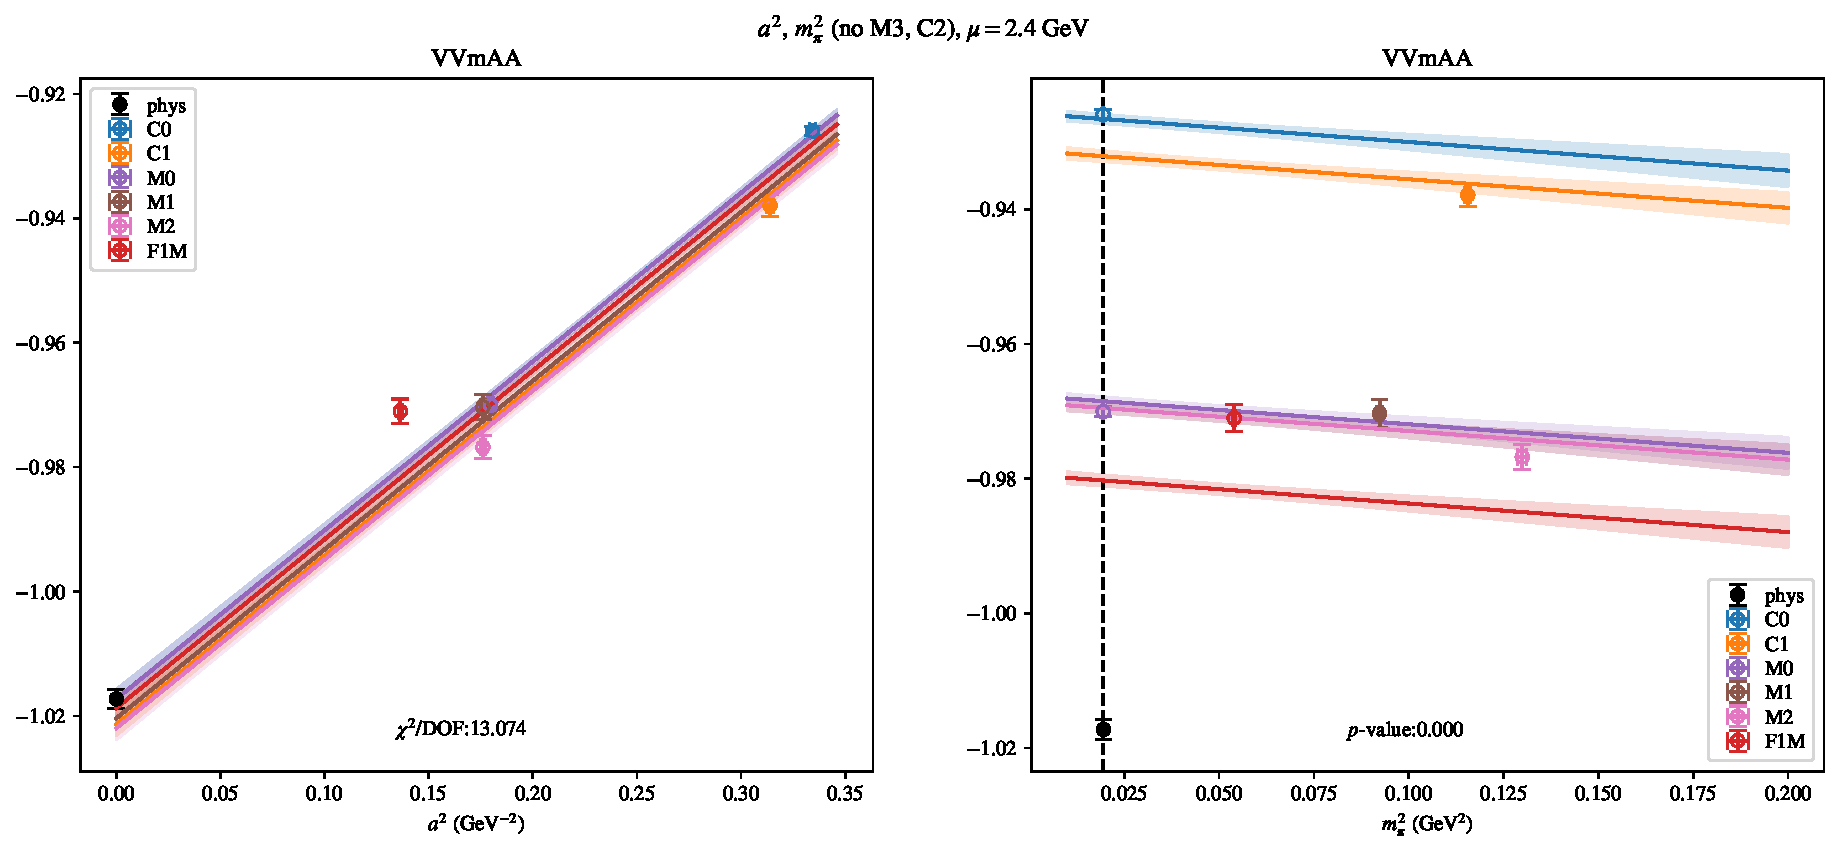
\includepdf[link, pages=-]{VVmAA/NPR/a2m2mcut_24.pdf}
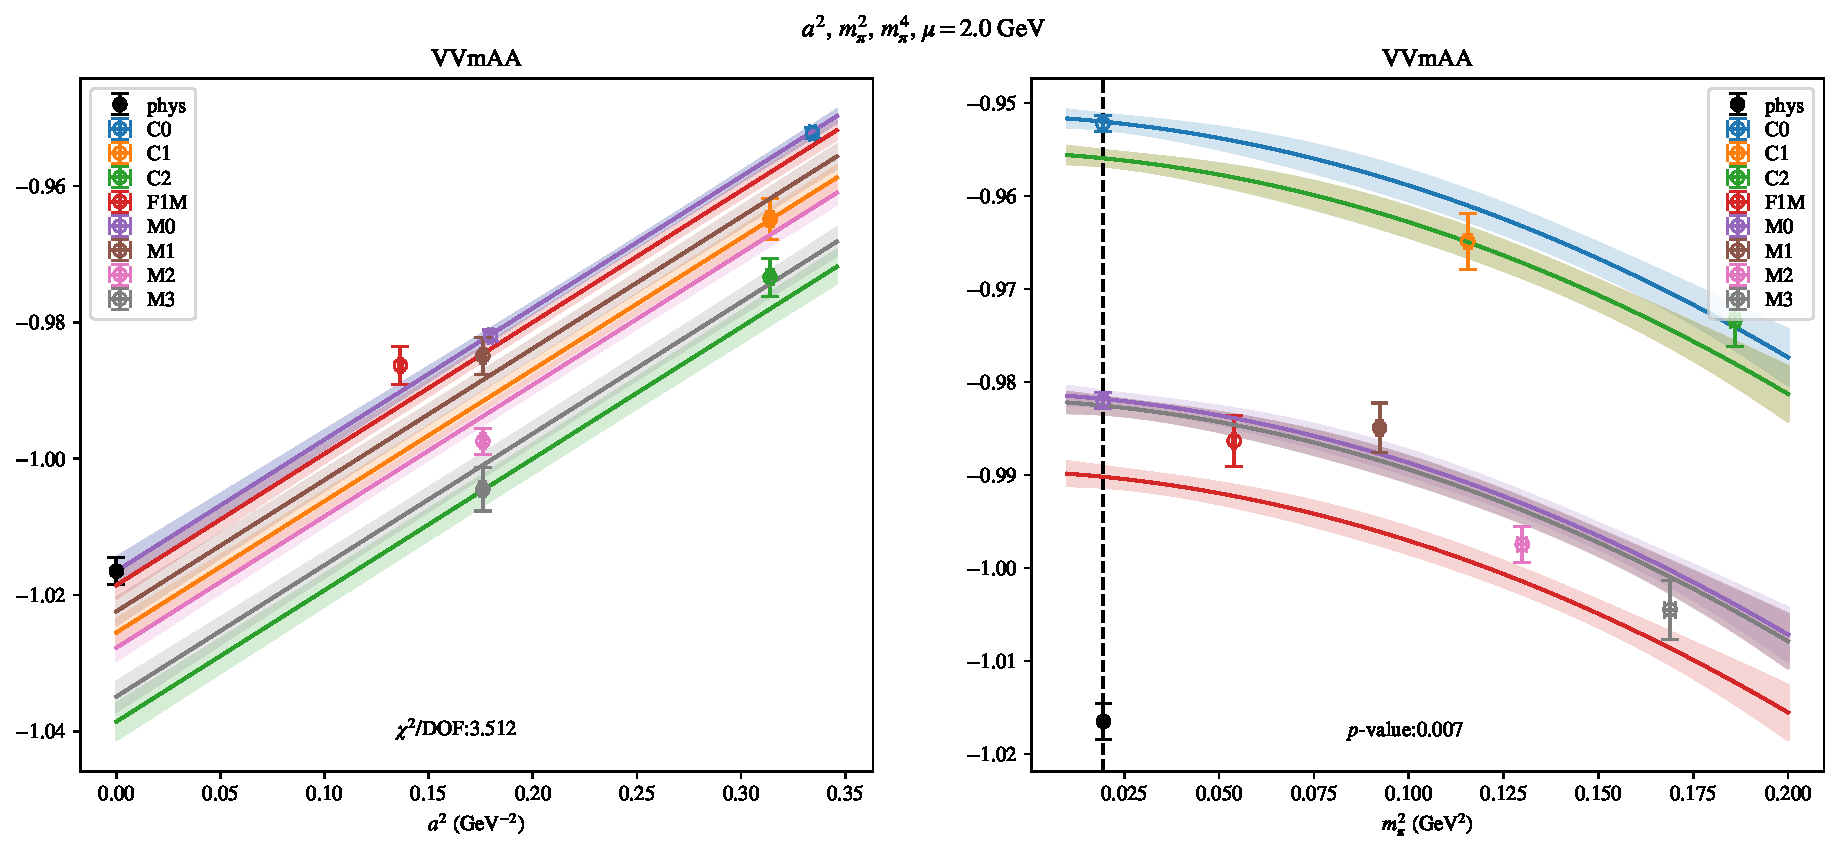
\includepdf[link, pages=-]{VVmAA/NPR/a2m2m4_20.pdf}
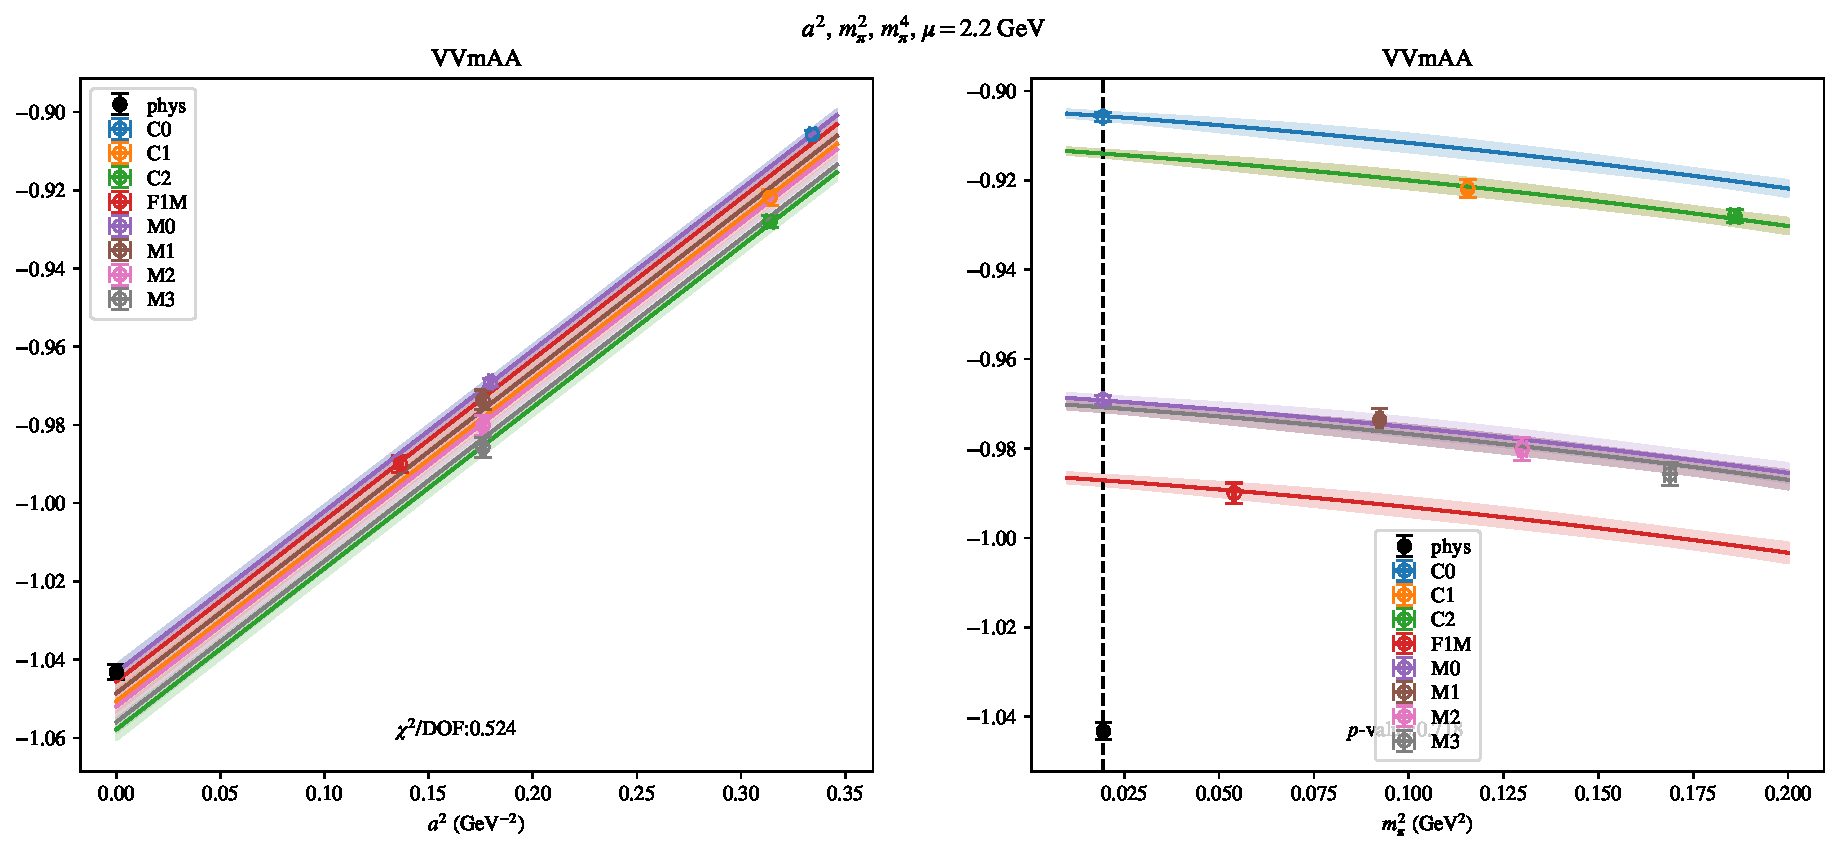
\includepdf[link, pages=-]{VVmAA/NPR/a2m2m4_22.pdf}
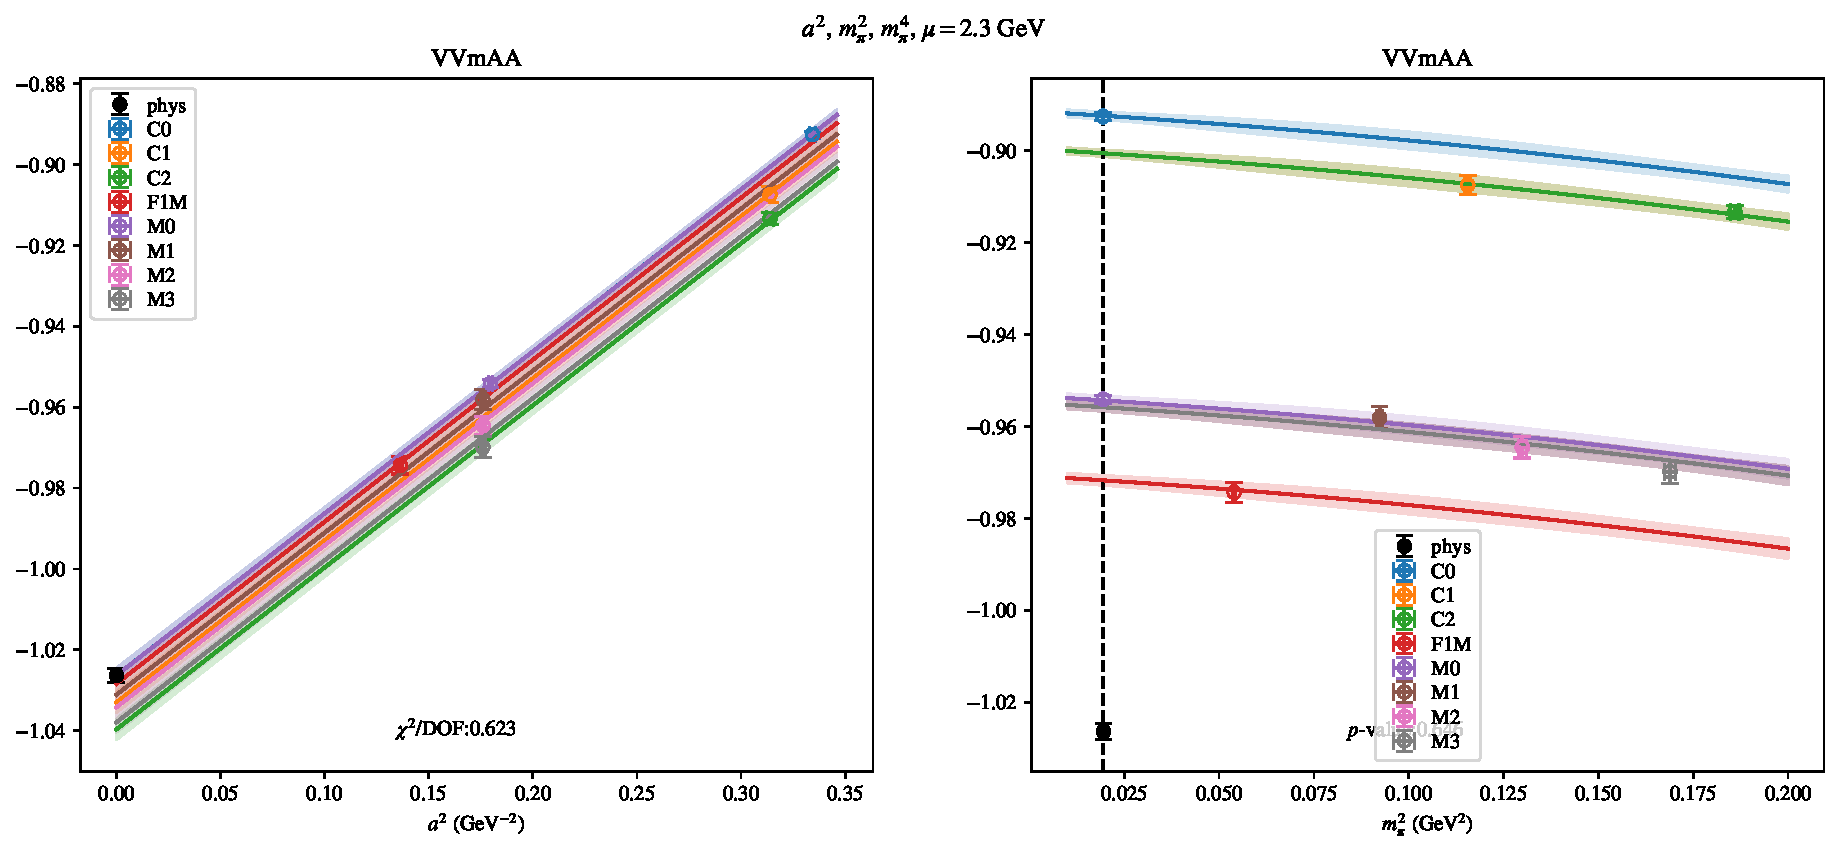
\includepdf[link, pages=-]{VVmAA/NPR/a2m2m4_23.pdf}
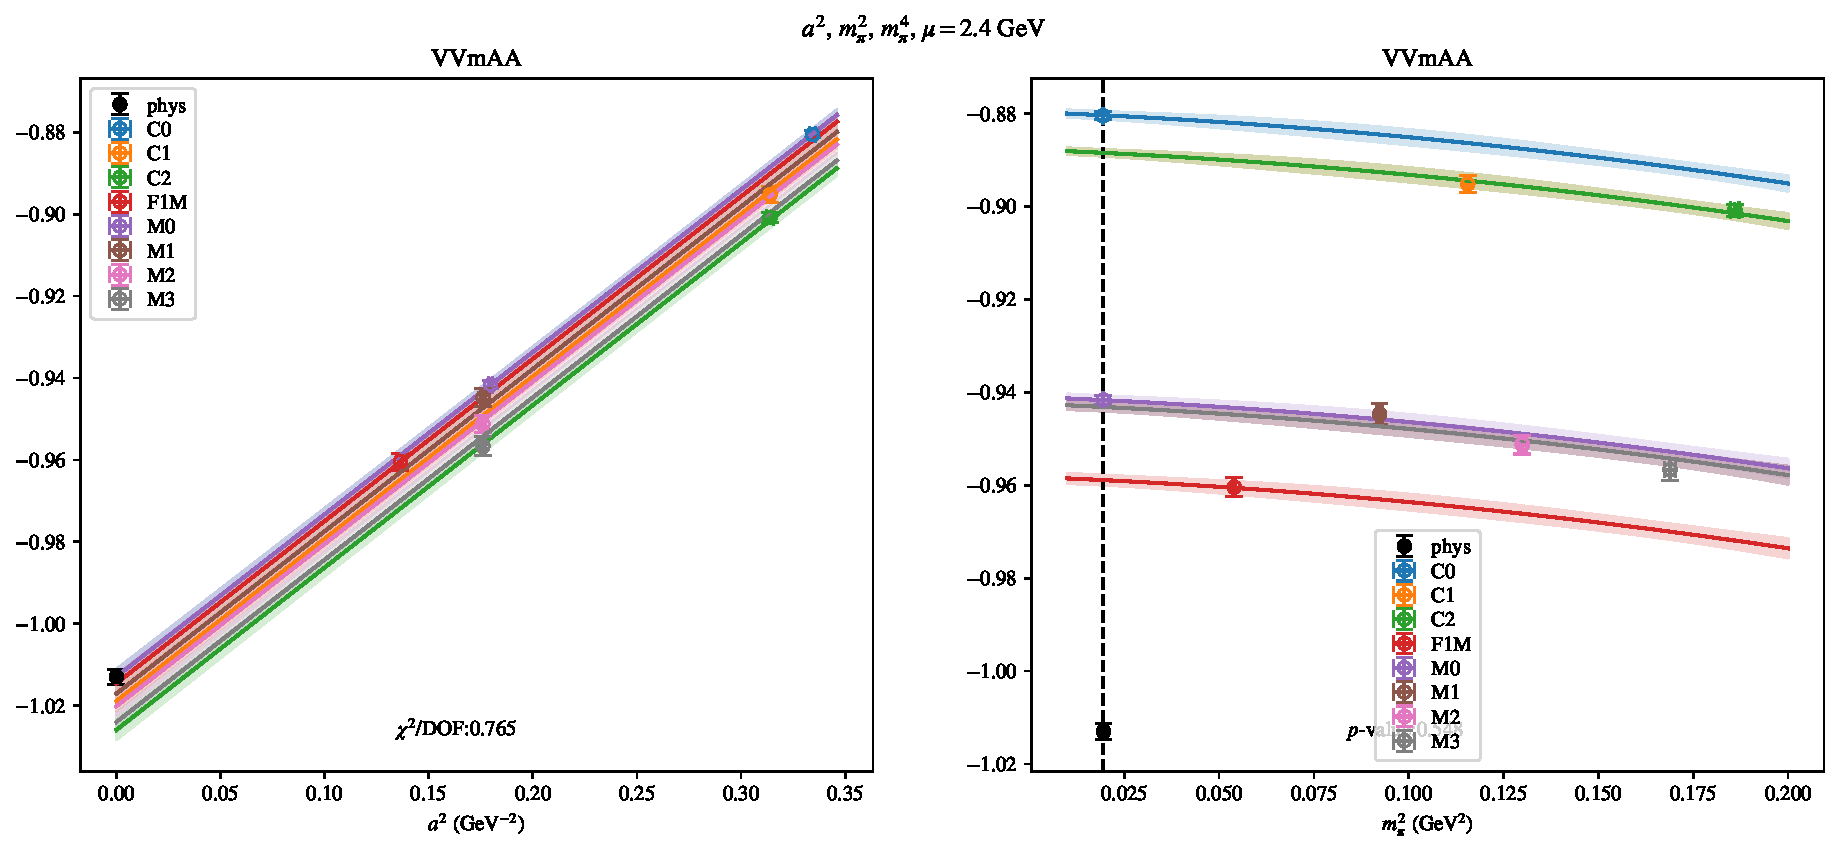
\includepdf[link, pages=-]{VVmAA/NPR/a2m2m4_24.pdf}
\clearpage
\section{$\mathcal{B}_3$}
\begin{table}[h!]
\begin{center}
\begin{tabular}{|c|c|c|c|c|c|}
\hline
$\mu$ (GeV) & $a^2$, $m_\pi^2$& $a^2$, $m_\pi^2$ (no C)& $a^2$, $a^4$, $m_\pi^2$& $a^2$, $m_\pi^2$ (no M3, C2)& $a^2$, $m_\pi^2$, $m_\pi^4$\\
\hline
2.0& \hyperlink{SSmPP/NPR/a2m2_20.pdf.1}{\textbf{1.8453(28)}: 5.593 (0.0)} & \hyperlink{SSmPP/NPR/a2m2noC_20.pdf.1}{\textbf{1.783(14)}: 2.936 (0.053)} & \hyperlink{SSmPP/NPR/a2a4m2_20.pdf.1}{\textbf{1.763(23)}: 3.766 (0.005)} & \hyperlink{SSmPP/NPR/a2m2mcut_20.pdf.1}{\textbf{1.8440(30)}: 6.702 (0.0)} & \hyperlink{SSmPP/NPR/a2m2m4_20.pdf.1}{\textbf{1.8482(31)}: 5.815 (0.0)}\\
2.2& \hyperlink{SSmPP/NPR/a2m2_22.pdf.1}{\textbf{1.8340(26)}: 5.464 (0.0)} & \hyperlink{SSmPP/NPR/a2m2noC_22.pdf.1}{\textbf{1.772(13)}: 1.972 (0.139)} & \hyperlink{SSmPP/NPR/a2a4m2_22.pdf.1}{\textbf{1.736(21)}: 1.478 (0.206)} & \hyperlink{SSmPP/NPR/a2m2mcut_22.pdf.1}{\textbf{1.8342(29)}: 7.967 (0.0)} & \hyperlink{SSmPP/NPR/a2m2m4_22.pdf.1}{\textbf{1.8373(29)}: 5.197 (0.0)}\\
2.3& \hyperlink{SSmPP/NPR/a2m2_23.pdf.1}{\textbf{1.8310(26)}: 5.824 (0.0)} & \hyperlink{SSmPP/NPR/a2m2noC_23.pdf.1}{\textbf{1.767(12)}: 2.094 (0.123)} & \hyperlink{SSmPP/NPR/a2a4m2_23.pdf.1}{\textbf{1.733(21)}: 1.773 (0.131)} & \hyperlink{SSmPP/NPR/a2m2mcut_23.pdf.1}{\textbf{1.8311(28)}: 8.437 (0.0)} & \hyperlink{SSmPP/NPR/a2m2m4_23.pdf.1}{\textbf{1.8346(29)}: 5.521 (0.0)}\\
2.4& \hyperlink{SSmPP/NPR/a2m2_24.pdf.1}{\textbf{1.8286(26)}: 6.51 (0.0)} & \hyperlink{SSmPP/NPR/a2m2noC_24.pdf.1}{\textbf{1.762(12)}: 2.441 (0.087)} & \hyperlink{SSmPP/NPR/a2a4m2_24.pdf.1}{\textbf{1.725(21)}: 1.934 (0.102)} & \hyperlink{SSmPP/NPR/a2m2mcut_24.pdf.1}{\textbf{1.8289(29)}: 9.482 (0.0)} & \hyperlink{SSmPP/NPR/a2m2m4_24.pdf.1}{\textbf{1.8323(29)}: 6.181 (0.0)}\\
\hline
\end{tabular}
\caption{Physical point value from chiral and continuum extrapolation at renormalisation scale $\mu$. Entries are \textbf{value(error)}: $\chi^2/\text{DOF}$ ($p$-value).}
\end{center}
\end{table}
\begin{table}[h!]
\begin{center}
\begin{tabular}{|c c|c|c|c|c|c|}
\hline
$\mu$ (GeV) &  & $a^2$, $m_\pi^2$& $a^2$, $m_\pi^2$ (no C)& $a^2$, $a^4$, $m_\pi^2$& $a^2$, $m_\pi^2$ (no M3, C2)& $a^2$, $m_\pi^2$, $m_\pi^4$\\
\hline
\multirow{2}{0.5in}{2.0} & $\alpha$ & 0.0627(58)& 0.261(47)& 0.48(12)& 0.0658(62)& 0.0575(64)\\
 & $\beta$ & -0.0002(15)& 0.00013(22)& -0.0003(17)& -0.0003(22)& -0.0017(66)\\
\hline
\multirow{2}{0.5in}{2.2} & $\alpha$ & 0.0703(56)& 0.273(44)& 0.57(11)& 0.0704(61)& 0.0642(61)\\
 & $\beta$ & -0.0002(12)& -0.0002(21)& -0.0004(14)& -0.0005(22)& -0.0019(64)\\
\hline
\multirow{2}{0.5in}{2.3} & $\alpha$ & 0.0711(54)& 0.281(44)& 0.58(12)& 0.0714(60)& 0.0644(61)\\
 & $\beta$ & -0.0003(13)& -0.0002(20)& -0.0005(14)& -0.0006(22)& -0.0021(64)\\
\hline
\multirow{2}{0.5in}{2.4} & $\alpha$ & 0.0721(55)& 0.292(44)& 0.61(11)& 0.0722(60)& 0.0654(60)\\
 & $\beta$ & -0.0003(12)& -0.0003(20)& -0.0006(13)& -0.0006(21)& -0.0021(63)\\
\hline
\end{tabular}
\caption{Fit values of coefficients in $Q = Q_{phys} + \mathbf{\alpha} a^2 + \mathbf{\beta}\left(\frac{m_\pi^2}{f_\pi^2}-\frac{m_{\pi,PDG}^2}{f_\pi^2}\right) + \ldots$.}
\end{center}
\end{table}
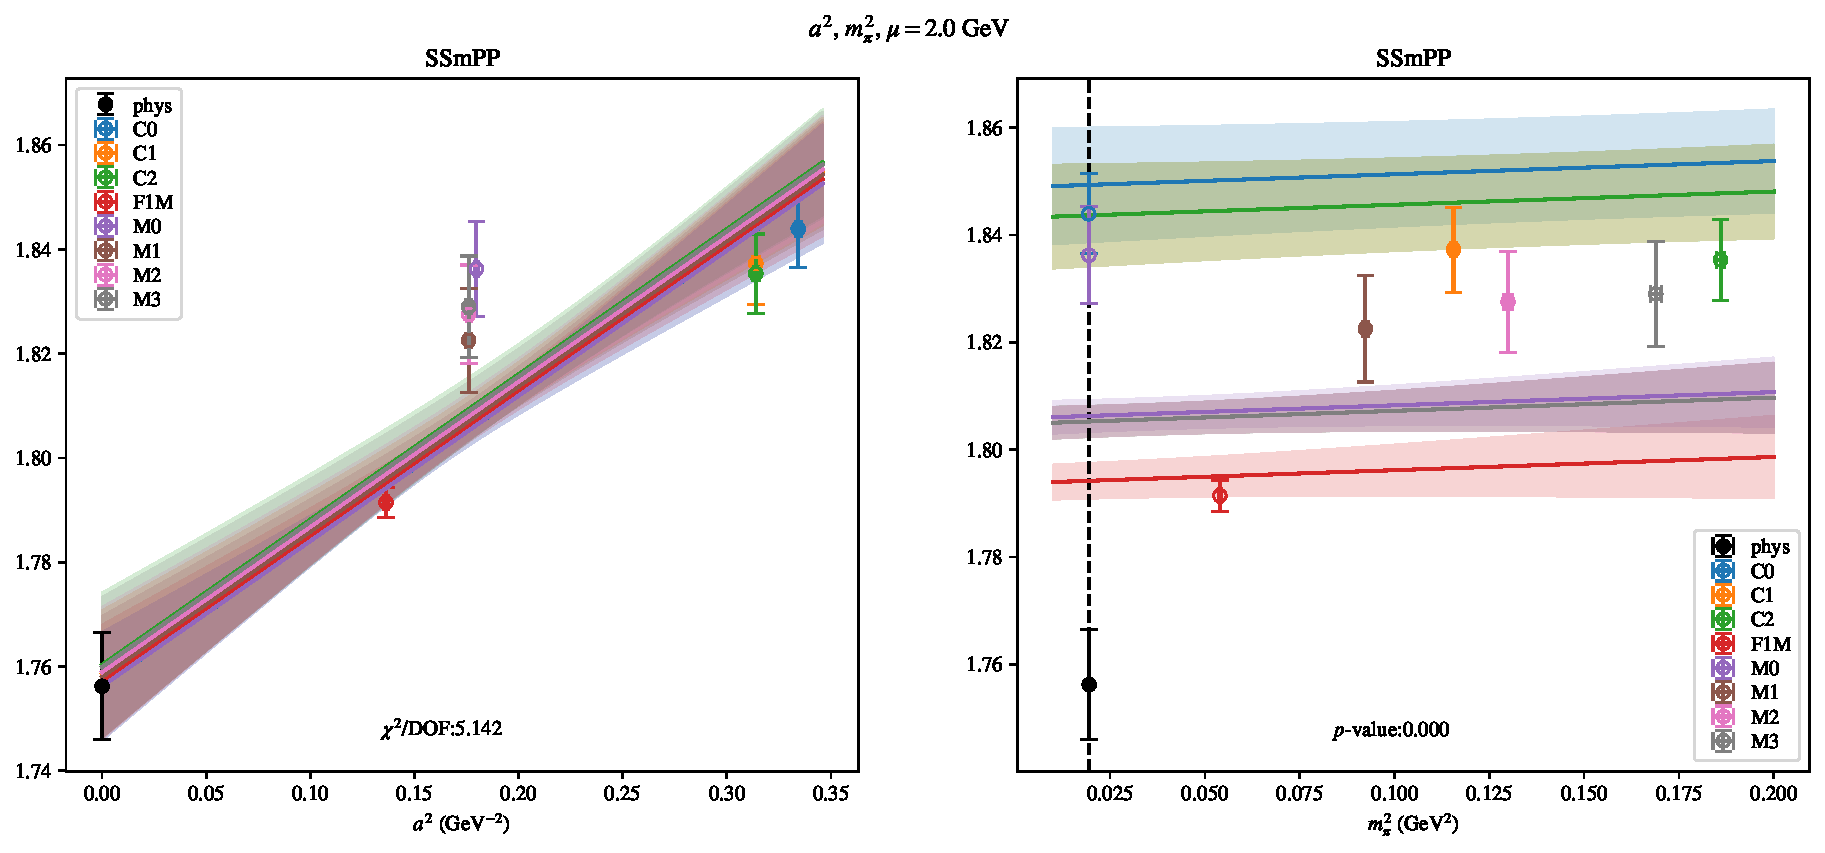
\includepdf[link, pages=-]{SSmPP/NPR/a2m2_20.pdf}
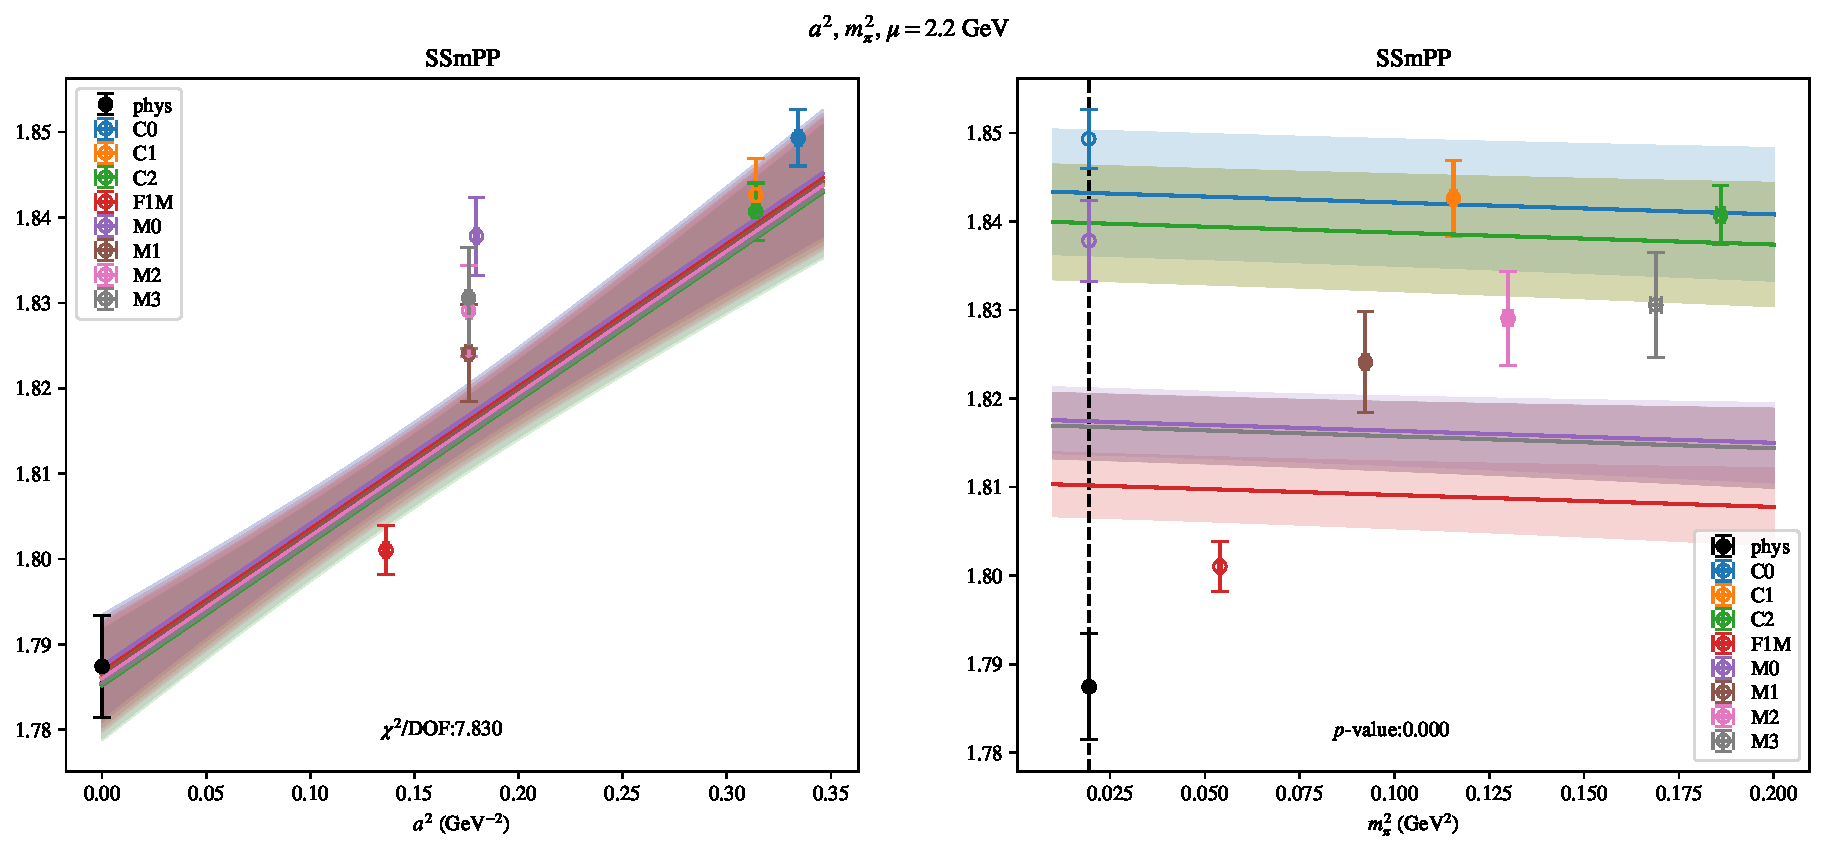
\includepdf[link, pages=-]{SSmPP/NPR/a2m2_22.pdf}
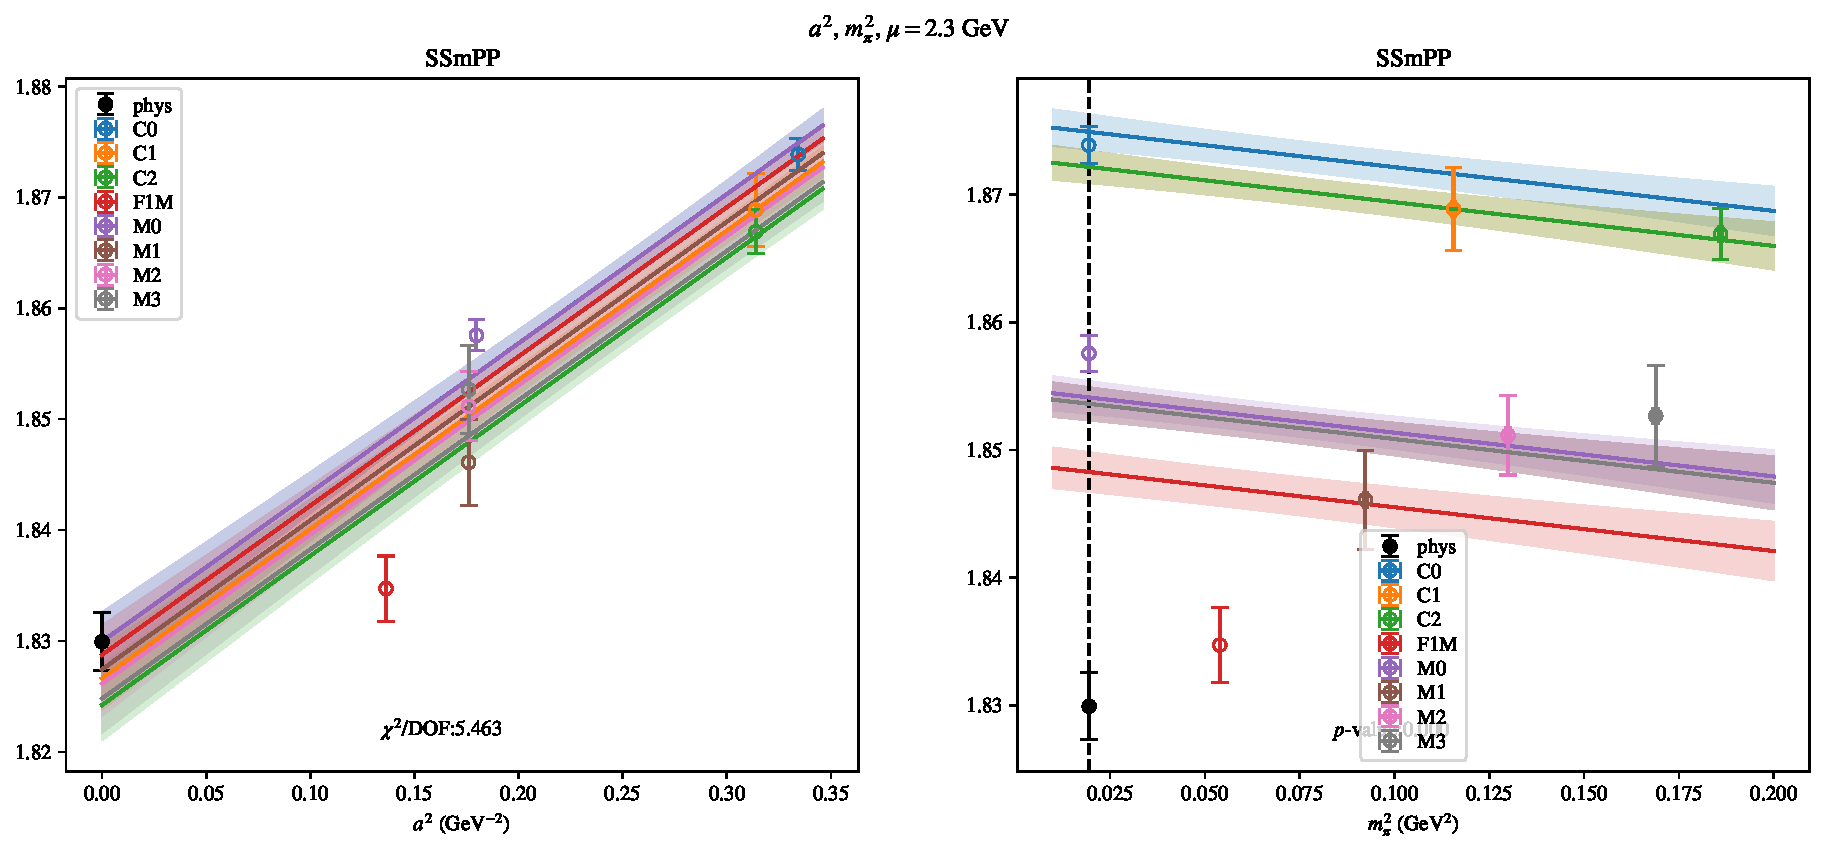
\includepdf[link, pages=-]{SSmPP/NPR/a2m2_23.pdf}
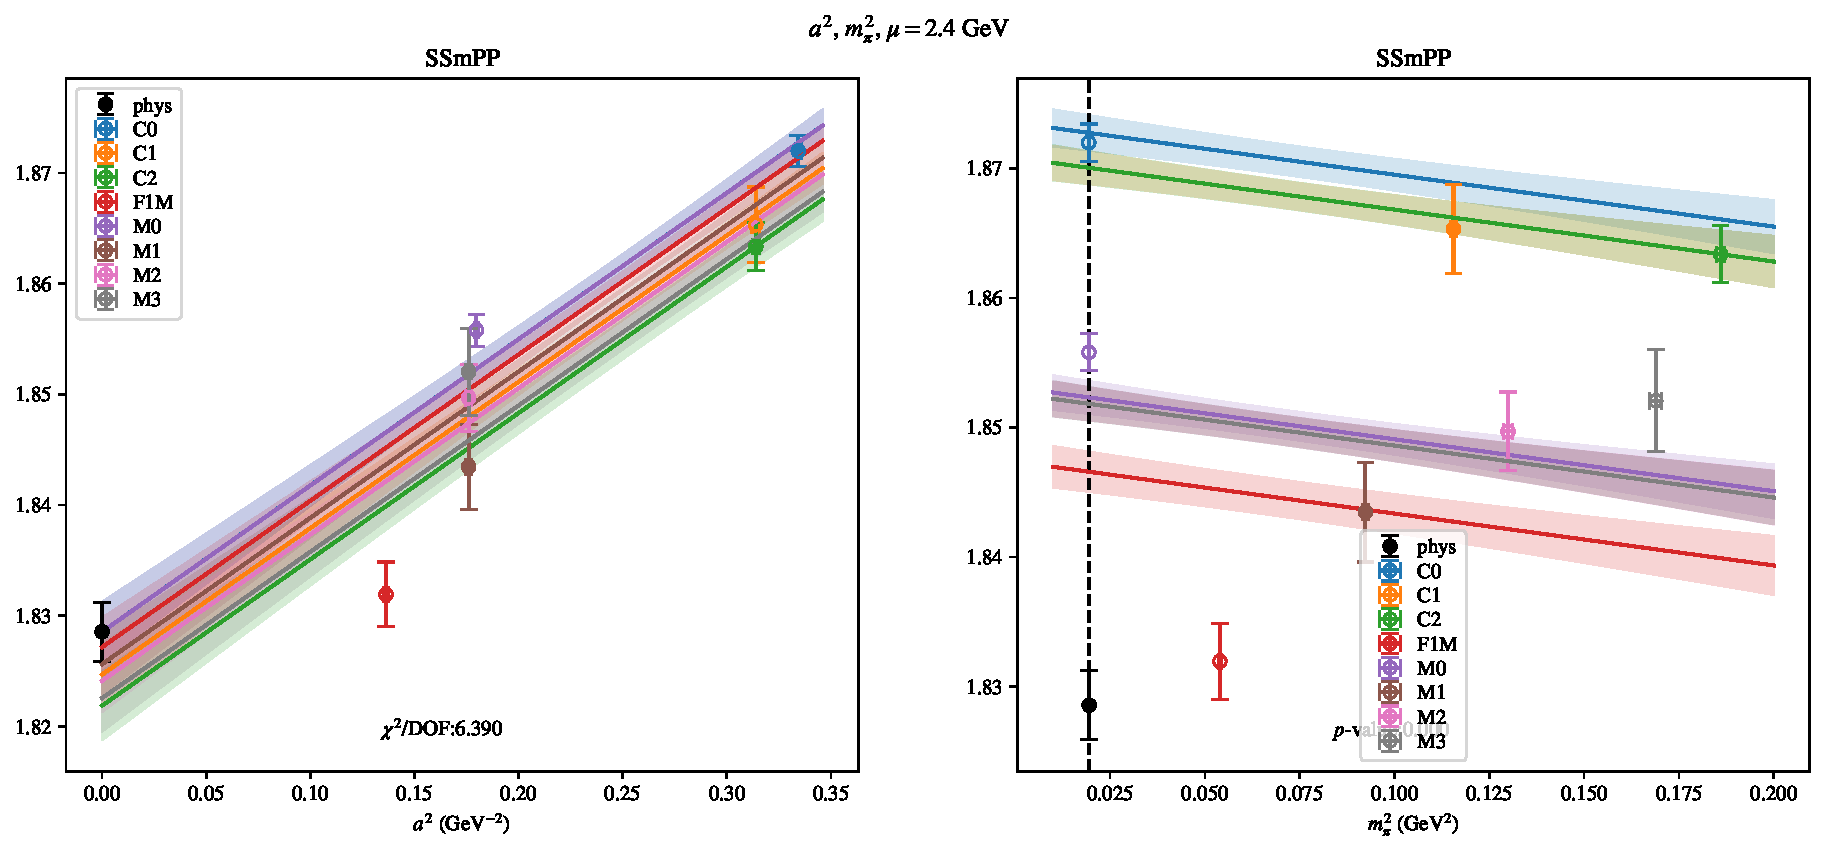
\includepdf[link, pages=-]{SSmPP/NPR/a2m2_24.pdf}
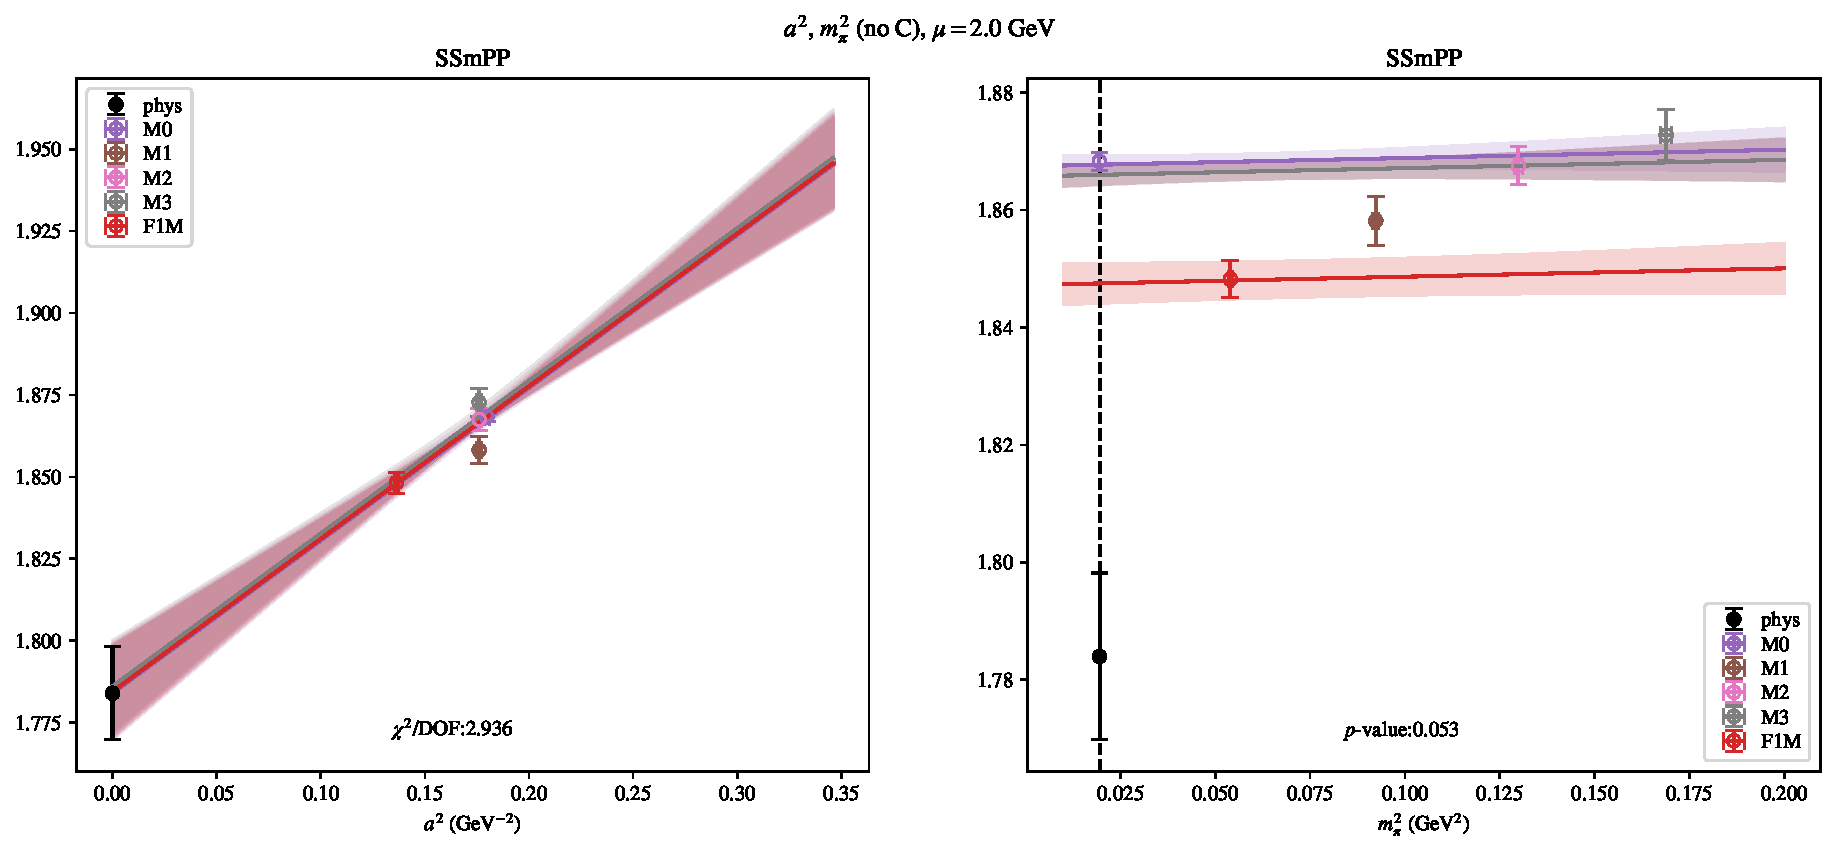
\includepdf[link, pages=-]{SSmPP/NPR/a2m2noC_20.pdf}
\includepdf[link, pages=-]{SSmPP/NPR/a2m2noC_22.pdf}
\includepdf[link, pages=-]{SSmPP/NPR/a2m2noC_23.pdf}
\includepdf[link, pages=-]{SSmPP/NPR/a2m2noC_24.pdf}
\includepdf[link, pages=-]{SSmPP/NPR/a2a4m2_20.pdf}
\includepdf[link, pages=-]{SSmPP/NPR/a2a4m2_22.pdf}
\includepdf[link, pages=-]{SSmPP/NPR/a2a4m2_23.pdf}
\includepdf[link, pages=-]{SSmPP/NPR/a2a4m2_24.pdf}
\includepdf[link, pages=-]{SSmPP/NPR/a2m2mcut_20.pdf}
\includepdf[link, pages=-]{SSmPP/NPR/a2m2mcut_22.pdf}
\includepdf[link, pages=-]{SSmPP/NPR/a2m2mcut_23.pdf}
\includepdf[link, pages=-]{SSmPP/NPR/a2m2mcut_24.pdf}
\includepdf[link, pages=-]{SSmPP/NPR/a2m2m4_20.pdf}
\includepdf[link, pages=-]{SSmPP/NPR/a2m2m4_22.pdf}
\includepdf[link, pages=-]{SSmPP/NPR/a2m2m4_23.pdf}
\includepdf[link, pages=-]{SSmPP/NPR/a2m2m4_24.pdf}
\clearpage
\section{$\mathcal{B}_4$}
\begin{table}[h!]
\begin{center}
\begin{tabular}{|c|c|c|c|c|c|}
\hline
$\mu$ (GeV) & $a^2$, $m_\pi^2$& $a^2$, $m_\pi^2$ (no C)& $a^2$, $a^4$, $m_\pi^2$& $a^2$, $m_\pi^2$ (no M3, C2)& $a^2$, $m_\pi^2$, $m_\pi^4$\\
\hline
2.0& \hyperlink{SSpPP/NPR/a2m2_20.pdf.1}{\textbf{-0.949(22)}: 3.599 (0.003)} & \hyperlink{SSpPP/NPR/a2m2noC_20.pdf.1}{\textbf{-0.98(10)}: 1.212 (0.298)} & \hyperlink{SSpPP/NPR/a2a4m2_20.pdf.1}{\textbf{-1.00(17)}: 1.63 (0.163)} & \hyperlink{SSpPP/NPR/a2m2mcut_20.pdf.1}{\textbf{-0.948(24)}: 5.271 (0.001)} & \hyperlink{SSpPP/NPR/a2m2m4_20.pdf.1}{\textbf{-0.946(24)}: 2.738 (0.027)}\\
2.2& \hyperlink{SSpPP/NPR/a2m2_22.pdf.1}{\textbf{-0.920(21)}: 4.988 (0.0)} & \hyperlink{SSpPP/NPR/a2m2noC_22.pdf.1}{\textbf{-0.956(96)}: 1.934 (0.145)} & \hyperlink{SSpPP/NPR/a2a4m2_22.pdf.1}{\textbf{-0.96(16)}: 4.291 (0.002)} & \hyperlink{SSpPP/NPR/a2m2mcut_22.pdf.1}{\textbf{-0.920(22)}: 6.696 (0.0)} & \hyperlink{SSpPP/NPR/a2m2m4_22.pdf.1}{\textbf{-0.917(23)}: 4.386 (0.002)}\\
2.3& \hyperlink{SSpPP/NPR/a2m2_23.pdf.1}{\textbf{-0.908(19)}: 4.6 (0.0)} & \hyperlink{SSpPP/NPR/a2m2noC_23.pdf.1}{\textbf{-0.944(93)}: 1.819 (0.162)} & \hyperlink{SSpPP/NPR/a2a4m2_23.pdf.1}{\textbf{-0.95(16)}: 3.603 (0.006)} & \hyperlink{SSpPP/NPR/a2m2mcut_23.pdf.1}{\textbf{-0.908(21)}: 6.277 (0.0)} & \hyperlink{SSpPP/NPR/a2m2m4_23.pdf.1}{\textbf{-0.906(22)}: 3.996 (0.003)}\\
2.4& \hyperlink{SSpPP/NPR/a2m2_24.pdf.1}{\textbf{-0.899(19)}: 4.597 (0.0)} & \hyperlink{SSpPP/NPR/a2m2noC_24.pdf.1}{\textbf{-0.931(92)}: 1.606 (0.201)} & \hyperlink{SSpPP/NPR/a2a4m2_24.pdf.1}{\textbf{-0.93(15)}: 4.222 (0.002)} & \hyperlink{SSpPP/NPR/a2m2mcut_24.pdf.1}{\textbf{-0.899(20)}: 6.18 (0.0)} & \hyperlink{SSpPP/NPR/a2m2m4_24.pdf.1}{\textbf{-0.897(21)}: 4.271 (0.002)}\\
\hline
\end{tabular}
\caption{Physical point value from chiral and continuum extrapolation at renormalisation scale $\mu$. Entries are \textbf{value(error)}: $\chi^2/\text{DOF}$ ($p$-value).}
\end{center}
\end{table}
\begin{table}[h!]
\begin{center}
\begin{tabular}{|c c|c|c|c|c|c|}
\hline
$\mu$ (GeV) &  & $a^2$, $m_\pi^2$& $a^2$, $m_\pi^2$ (no C)& $a^2$, $a^4$, $m_\pi^2$& $a^2$, $m_\pi^2$ (no M3, C2)& $a^2$, $m_\pi^2$, $m_\pi^4$\\
\hline
\multirow{2}{0.5in}{2.0} & $\alpha$ & 0.3667(97)& 0.133(63)& -0.1(15)& 0.371(10)& 0.376(10)\\
 & $\beta$ & 0.00746(21)& 0.00725(25)& 0.00721(21)& 0.00784(30)& 0.01003(86)\\
\hline
\multirow{2}{0.5in}{2.2} & $\alpha$ & 0.4157(97)& 0.185(60)& -0.0& 0.4151(99)& 0.424(10)\\
 & $\beta$ & 0.00752(19)& 0.00690(23)& 0.00730(21)& 0.00788(28)& 0.00998(80)\\
\hline
\multirow{2}{0.5in}{2.3} & $\alpha$ & 0.4360(90)& 0.207(59)& 0.004& 0.4359(99)& 0.444(10)\\
 & $\beta$ & 0.00745(20)& 0.00688(23)& 0.00723(21)& 0.00781(29)& 0.00987(83)\\
\hline
\multirow{2}{0.5in}{2.4} & $\alpha$ & 0.4542(91)& 0.245(59)& 0.10(15)& 0.4537(96)& 0.462(10)\\
 & $\beta$ & 0.00750(18)& 0.00686(22)& 0.00733(20)& 0.00784(28)& 0.00967(79)\\
\hline
\end{tabular}
\caption{Fit values of coefficients in $Q = Q_{phys} + \mathbf{\alpha} a^2 + \mathbf{\beta}\left(\frac{m_\pi^2}{f_\pi^2}-\frac{m_{\pi,PDG}^2}{f_\pi^2}\right) + \ldots$.}
\end{center}
\end{table}
\includepdf[link, pages=-]{SSpPP/NPR/a2m2_20.pdf}
\includepdf[link, pages=-]{SSpPP/NPR/a2m2_22.pdf}
\includepdf[link, pages=-]{SSpPP/NPR/a2m2_23.pdf}
\includepdf[link, pages=-]{SSpPP/NPR/a2m2_24.pdf}
\includepdf[link, pages=-]{SSpPP/NPR/a2m2noC_20.pdf}
\includepdf[link, pages=-]{SSpPP/NPR/a2m2noC_22.pdf}
\includepdf[link, pages=-]{SSpPP/NPR/a2m2noC_23.pdf}
\includepdf[link, pages=-]{SSpPP/NPR/a2m2noC_24.pdf}
\includepdf[link, pages=-]{SSpPP/NPR/a2a4m2_20.pdf}
\includepdf[link, pages=-]{SSpPP/NPR/a2a4m2_22.pdf}
\includepdf[link, pages=-]{SSpPP/NPR/a2a4m2_23.pdf}
\includepdf[link, pages=-]{SSpPP/NPR/a2a4m2_24.pdf}
\includepdf[link, pages=-]{SSpPP/NPR/a2m2mcut_20.pdf}
\includepdf[link, pages=-]{SSpPP/NPR/a2m2mcut_22.pdf}
\includepdf[link, pages=-]{SSpPP/NPR/a2m2mcut_23.pdf}
\includepdf[link, pages=-]{SSpPP/NPR/a2m2mcut_24.pdf}
\includepdf[link, pages=-]{SSpPP/NPR/a2m2m4_20.pdf}
\includepdf[link, pages=-]{SSpPP/NPR/a2m2m4_22.pdf}
\includepdf[link, pages=-]{SSpPP/NPR/a2m2m4_23.pdf}
\includepdf[link, pages=-]{SSpPP/NPR/a2m2m4_24.pdf}
\clearpage
\section{$\mathcal{B}_5$}
\begin{table}[h!]
\begin{center}
\begin{tabular}{|c|c|c|c|c|c|}
\hline
$\mu$ (GeV) & $a^2$, $m_\pi^2$& $a^2$, $m_\pi^2$ (no C)& $a^2$, $a^4$, $m_\pi^2$& $a^2$, $m_\pi^2$ (no M3, C2)& $a^2$, $m_\pi^2$, $m_\pi^4$\\
\hline
2.0& \hyperlink{TT/NPR/a2m2_20.pdf.1}{\textbf{-0.371(10)}: 1.313 (0.255)} & \hyperlink{TT/NPR/a2m2noC_20.pdf.1}{\textbf{-0.383(53)}: 0.14 (0.87)} & \hyperlink{TT/NPR/a2a4m2_20.pdf.1}{\textbf{-0.391(88)}: 0.182 (0.948)} & \hyperlink{TT/NPR/a2m2mcut_20.pdf.1}{\textbf{-0.370(10)}: 2.08 (0.101)} & \hyperlink{TT/NPR/a2m2m4_20.pdf.1}{\textbf{-0.370(11)}: 1.462 (0.211)}\\
2.2& \hyperlink{TT/NPR/a2m2_22.pdf.1}{\textbf{-0.3653(91)}: 1.642 (0.145)} & \hyperlink{TT/NPR/a2m2noC_22.pdf.1}{\textbf{-0.376(43)}: 0.142 (0.868)} & \hyperlink{TT/NPR/a2a4m2_22.pdf.1}{\textbf{-0.380(75)}: 0.853 (0.491)} & \hyperlink{TT/NPR/a2m2mcut_22.pdf.1}{\textbf{-0.3654(97)}: 2.656 (0.047)} & \hyperlink{TT/NPR/a2m2m4_22.pdf.1}{\textbf{-0.365(10)}: 1.846 (0.117)}\\
2.3& \hyperlink{TT/NPR/a2m2_23.pdf.1}{\textbf{-0.3631(93)}: 1.432 (0.209)} & \hyperlink{TT/NPR/a2m2noC_23.pdf.1}{\textbf{-0.373(42)}: 0.143 (0.867)} & \hyperlink{TT/NPR/a2a4m2_23.pdf.1}{\textbf{-0.376(72)}: 0.795 (0.528)} & \hyperlink{TT/NPR/a2m2mcut_23.pdf.1}{\textbf{-0.3632(95)}: 2.299 (0.075)} & \hyperlink{TT/NPR/a2m2m4_23.pdf.1}{\textbf{-0.3628(96)}: 1.609 (0.169)}\\
2.4& \hyperlink{TT/NPR/a2m2_24.pdf.1}{\textbf{-0.3613(85)}: 1.317 (0.253)} & \hyperlink{TT/NPR/a2m2noC_24.pdf.1}{\textbf{-0.370(41)}: 0.184 (0.832)} & \hyperlink{TT/NPR/a2a4m2_24.pdf.1}{\textbf{-0.372(71)}: 1.0 (0.406)} & \hyperlink{TT/NPR/a2m2mcut_24.pdf.1}{\textbf{-0.3614(89)}: 2.029 (0.107)} & \hyperlink{TT/NPR/a2m2m4_24.pdf.1}{\textbf{-0.3610(95)}: 1.456 (0.213)}\\
\hline
\end{tabular}
\caption{Physical point value from chiral and continuum extrapolation at renormalisation scale $\mu$. Entries are \textbf{value(error)}: $\chi^2/\text{DOF}$ ($p$-value).}
\end{center}
\end{table}
\begin{table}[h!]
\begin{center}
\begin{tabular}{|c c|c|c|c|c|c|}
\hline
$\mu$ (GeV) &  & $a^2$, $m_\pi^2$& $a^2$, $m_\pi^2$ (no C)& $a^2$, $a^4$, $m_\pi^2$& $a^2$, $m_\pi^2$ (no M3, C2)& $a^2$, $m_\pi^2$, $m_\pi^4$\\
\hline
\multirow{2}{0.5in}{2.0} & $\alpha$ & -0.04(10)& -0.22(76)& -0.5(19)& -0.03(10)& -0.03(10)\\
 & $\beta$ & 0.00708(31)& 0.00687(35)& 0.00681(31)& 0.00714(37)& 0.0081(10)\\
\hline
\multirow{2}{0.5in}{2.2} & $\alpha$ & -0.084(94)& -0.25(64)& -0.4(16)& -0.085(98)& -0.08(10)\\
 & $\beta$ & 0.00680(24)& 0.00643(28)& 0.00661(27)& 0.00683(33)& 0.00764(92)\\
\hline
\multirow{2}{0.5in}{2.3} & $\alpha$ & -0.108(95)& -0.25(63)& -0.4(16)& -0.109(95)& -0.105(96)\\
 & $\beta$ & 0.00673(25)& 0.00640(28)& 0.00658(27)& 0.00677(33)& 0.00765(93)\\
\hline
\multirow{2}{0.5in}{2.4} & $\alpha$ & -0.132(89)& -0.26(62)& -0.3(16)& -0.133(90)& -0.130(96)\\
 & $\beta$ & 0.00668(22)& 0.00635(25)& 0.00657(23)& 0.00670(31)& 0.00743(90)\\
\hline
\end{tabular}
\caption{Fit values of coefficients in $Q = Q_{phys} + \mathbf{\alpha} a^2 + \mathbf{\beta}\left(\frac{m_\pi^2}{f_\pi^2}-\frac{m_{\pi,PDG}^2}{f_\pi^2}\right) + \ldots$.}
\end{center}
\end{table}
\includepdf[link, pages=-]{TT/NPR/a2m2_20.pdf}
\includepdf[link, pages=-]{TT/NPR/a2m2_22.pdf}
\includepdf[link, pages=-]{TT/NPR/a2m2_23.pdf}
\includepdf[link, pages=-]{TT/NPR/a2m2_24.pdf}
\includepdf[link, pages=-]{TT/NPR/a2m2noC_20.pdf}
\includepdf[link, pages=-]{TT/NPR/a2m2noC_22.pdf}
\includepdf[link, pages=-]{TT/NPR/a2m2noC_23.pdf}
\includepdf[link, pages=-]{TT/NPR/a2m2noC_24.pdf}
\includepdf[link, pages=-]{TT/NPR/a2a4m2_20.pdf}
\includepdf[link, pages=-]{TT/NPR/a2a4m2_22.pdf}
\includepdf[link, pages=-]{TT/NPR/a2a4m2_23.pdf}
\includepdf[link, pages=-]{TT/NPR/a2a4m2_24.pdf}
\includepdf[link, pages=-]{TT/NPR/a2m2mcut_20.pdf}
\includepdf[link, pages=-]{TT/NPR/a2m2mcut_22.pdf}
\includepdf[link, pages=-]{TT/NPR/a2m2mcut_23.pdf}
\includepdf[link, pages=-]{TT/NPR/a2m2mcut_24.pdf}
\includepdf[link, pages=-]{TT/NPR/a2m2m4_20.pdf}
\includepdf[link, pages=-]{TT/NPR/a2m2m4_22.pdf}
\includepdf[link, pages=-]{TT/NPR/a2m2m4_23.pdf}
\includepdf[link, pages=-]{TT/NPR/a2m2m4_24.pdf}
\clearpage
\end{document}